\documentclass[a4paper]{book}
\usepackage{makeidx}
\usepackage{graphicx}
\usepackage{multicol}
\usepackage{float}
\usepackage{listings}
\usepackage{color}
\usepackage{ifthen}
\usepackage[table]{xcolor}
\usepackage{textcomp}
\usepackage{alltt}
\usepackage{ifpdf}
\ifpdf
\usepackage[pdftex,
            pagebackref=true,
            colorlinks=true,
            linkcolor=blue,
            unicode
           ]{hyperref}
\else
\usepackage[ps2pdf,
            pagebackref=true,
            colorlinks=true,
            linkcolor=blue,
            unicode
           ]{hyperref}
\usepackage{pspicture}
\fi
\usepackage[utf8]{inputenc}
\usepackage{mathptmx}
\usepackage[scaled=.90]{helvet}
\usepackage{courier}
\usepackage{doxygen}
\lstset{language=C++,inputencoding=utf8,basicstyle=\footnotesize,breaklines=true,breakatwhitespace=true,tabsize=8,numbers=left }
\makeindex
\setcounter{tocdepth}{3}
\renewcommand{\footrulewidth}{0.4pt}
\begin{document}
\hypersetup{pageanchor=false}
\begin{titlepage}
\vspace*{7cm}
\begin{center}
{\Large TinyImageLoader \\[1ex]\large 1.5.5 }\\
\vspace*{1cm}
{\large Generated by Doxygen 1.7.3}\\
\vspace*{0.5cm}
{\small Thu Mar 3 2011 09:56:07}\\
\end{center}
\end{titlepage}
\clearemptydoublepage
\pagenumbering{roman}
\tableofcontents
\clearemptydoublepage
\pagenumbering{arabic}
\hypersetup{pageanchor=true}
\chapter{TinyImageLoader}
\label{index}\hypertarget{index}{}TinyImageLoader is a library for loading images. It is designed to be cross-\/ platform, device-\/independent, fast and free (as in freedom).\hypertarget{index_About}{}\section{About}\label{index_About}

\begin{DoxyEnumerate}
\item \hyperlink{design}{Design}
\item \hyperlink{bugs}{Known bugs and issues} 
\end{DoxyEnumerate}\hypertarget{index_Examples}{}\section{Examples}\label{index_Examples}

\begin{DoxyEnumerate}
\item \hyperlink{example1}{Example: Loading an OpenGL texture} 
\end{DoxyEnumerate}
\chapter{Known bugs and issues}
\label{bugs}
\hypertarget{bugs}{}
I can do a lot, but not everything. These are the things I haven't gotten to.\hypertarget{bugs_colors1}{}\section{Color functions}\label{bugs_colors1}
Not all color formats are fully supported yet. What I've done is support at least all the construct functions. The rest will be done at a later time.\hypertarget{bugs_colors2}{}\section{Color conversion}\label{bugs_colors2}
Color conversion is a nightmare. They just keep on stacking. Right now there are 8 different color formats. That means there are 8 $\ast$ 7 = 56 color conversion functions (!). I've only implemented the ones I needed.\hypertarget{bugs_cmaaaaake}{}\section{CMake}\label{bugs_cmaaaaake}
There is no CMake for TinyImageLoader. I know this is annoying for a lot of people. I know I'm a big jerk. But I would like to bring up the following points:


\begin{DoxyItemize}
\item CMake doesn't use Visual Studio macros
\end{DoxyItemize}

CMake doesn't use Visual Studio macros in its paths. This is extremely annoying when your main development environment is Visual Studio. Paths become long and unreadable.

The official stance of CMake is that they don't care if it looks good, as long as it works. This is unacceptable to me.


\begin{DoxyItemize}
\item CMake doesn't give me enough control
\end{DoxyItemize}

I want my intermediate files in a directory labeled \char`\"{}int\char`\"{}. In that folder, I want two folders: \char`\"{}Debug\char`\"{} and \char`\"{}Release\char`\"{}. This is impossible to do in CMake, because it doesn't allow you to set the intermediate directory in Visual Studio.

Worse, for a long time it was hardly possible to set the output directory. You had to use what is known as the \char`\"{}backslash hack\char`\"{} to set the output directory. You set the dir to \char`\"{}$\backslash$..$\backslash$bin\char`\"{} so the path becomes \char`\"{}$<$Project$>$$\backslash$Debug$\backslash$..$\backslash$bin\char`\"{}.

Ugly.


\begin{DoxyItemize}
\item CMake has horrible documentation
\end{DoxyItemize}

The entire documentation to CMake is one giant HTML file. I'm not kidding. It's huge. You can try searching through it, but you'll inevitably end up lost and confused.

Which brings me to...


\begin{DoxyItemize}
\item CMake has no examples
\end{DoxyItemize}

The way to learn CMake is basically to look at other projects that use CMake and try stealing bits and pieces from it. But the structure of commands oftentimes doesn't make sense and the documention is no help either.


\begin{DoxyItemize}
\item CMake has no alternative
\end{DoxyItemize}

This is the worst thing. CMake doesn't do what I want and I have no alternatives besides maintaining vcproj's, vcxproj's and makefiles by hand.

Until something better comes along, or CMake fixes its flaws, I will be sticking to handmade Visual Studio project files. 
\chapter{Design}
\label{design}
\hypertarget{design}{}
The goal of TinyImageLoader was to create a library that only loads images. It does color conversion, but nothing else. Therefor, the following design choices have been made.\hypertarget{design_interface}{}\section{Simple interface}\label{design_interface}
An interface that makes it as easy as possible to load an image.


\begin{DoxyItemize}
\item include \hyperlink{_tiny_image_loader_8h}{TinyImageLoader.h}
\item call \hyperlink{namespacetil_a84a20b430c5ae27956968ef6d7a6425b}{til::TIL\_\-Init}
\item call \hyperlink{namespacetil_a8d2e2ab942bb94b188587509ccb754de}{til::TIL\_\-Load}
\item extract data
\item call \hyperlink{namespacetil_a777e336727a478c4c4bdfd8c0e3603d7}{til::TIL\_\-ShutDown}
\end{DoxyItemize}

TinyImageLoader knows it is only a middleman. It exposes all its methods without fluff. There is no multiple inheritance. There is only the Image interface with its clear and descriptive method names.

You can keep the Image handles around after loading or you can copy the data to your own data structures. The choice is up to you.\hypertarget{design_extensibility}{}\section{Extensibility}\label{design_extensibility}
Despite the easy interface, TinyImageLoader can also be extended. You can write your own implementation of \hyperlink{classtil_1_1_file_stream}{til::FileStream} and attach it to TinyImageLoader. You can set the logging callback to output to a file by using \hyperlink{namespacetil_acf5fe389d33053c01da96da10ef88b0e}{TIL\_\-SetErrorFunc()}. You can even compile TinyImageLoader to only support a single format by setting a single define in the preprocessor definitions (\hyperlink{_t_i_l_settings_8h_ae0783dd47fcd9fe85766834d4fa8006d}{TIL\_\-FORMAT}).\hypertarget{design_speed}{}\section{Speed}\label{design_speed}
Speed is a priority, but no platform-\/specific hacks are used. If a loader doesn't work as expected on another platform then that is considered a bug. 
\chapter{Example: Loading an OpenGL texture}
\label{example1}
\hypertarget{example1}{}
This example will show you how to load an image using TinyImageLoader and use it as a texture.\hypertarget{example1_intro}{}\section{Introduction}\label{example1_intro}
When you drag an image onto the exe created by this example, TinyImageLoader will try to load it. If the file cannot be loaded (for whatever the reason), you can check the til.log located at in /examples/bin/til.log. If you find an image that doesn't load, please send it and the log to me! I will get back to you as soon as possible with (hopefully) a fix and (always) an apology.\hypertarget{example1_input}{}\section{Key binding}\label{example1_input}
Use the following keys in this example:
\begin{DoxyItemize}
\item Q: Go to the next frame (if it exists)
\item W: Go to the previous frame (if it exists)
\item O: Zoom out on the image
\item P: Zoom in on the image
\end{DoxyItemize}\hypertarget{example1_setup}{}\section{Setup}\label{example1_setup}
There are a couple of things you need to do before you can start using TinyImageLoader. First, you need to compile the TinyImageLoader static library using Visual Studio. Then you can copy the SDK folder to a project. Here's how I set up my projects:
\begin{DoxyItemize}
\item $\backslash$ (project root)
\begin{DoxyItemize}
\item bin (output directory)
\begin{DoxyItemize}
\item Project.exe (Release build)
\item Project\_\-d.exe (Debug build)
\end{DoxyItemize}
\item int (intermediate directory)
\begin{DoxyItemize}
\item Debug
\item Release
\end{DoxyItemize}
\item lib (third-\/party libraries)
\begin{DoxyItemize}
\item TinyImageLoader
\begin{DoxyItemize}
\item TinyImageLoader.lib
\item TinyImageLoader\_\-d.lib
\item headers
\end{DoxyItemize}
\end{DoxyItemize}
\item src (project source files)
\item Project.vcproj
\item Solution.sln
\end{DoxyItemize}
\end{DoxyItemize}

You are free to set these things as you like, of course, but this is how I prefer it. :)\hypertarget{example1_startup}{}\section{Setting up TinyImageLoader}\label{example1_startup}
The first thing we need to do is initialize TinyImageLoader. 
\begin{DoxyCode}
        til::TIL_Init();
\end{DoxyCode}
\hypertarget{example1_logging}{}\section{Logging}\label{example1_logging}
By default, TinyImageLoader posts its errors and warning to an internal expanding string. This may not be desirable, as it takes memory you don't have any control over. Therefor, TinyImageLoader comes with a series of callbacks you can use to control the logging behavior.

In this example we will output all debug and error messages to a log.

We open our log by using a TinyImageLoader function to attach the working directory. 
\begin{DoxyCode}
        g_LogPath = new char[TIL_MAX_PATH];
        til::TIL_AddWorkingDirectory(g_LogPath, TIL_MAX_PATH, "til.log");
        fopen_s(&g_Log, g_LogPath, "w+");
        fclose(g_Log);
\end{DoxyCode}


We open it only to clear it. If it doesn't exist it gets created.

We have a custom logging function, that outputs the message to the log we just created.


\begin{DoxyCode}
        void LoggingFunc(til::MessageData* a_Data)
        {
                fopen_s(&g_Log, g_LogPath, "a");
                char msg[1024];
                //sprintf_s(msg, "%s (at line %i in file %s)", a_Data->message, a
      _Data->source_line, a_Data->source_file);
                sprintf_s(msg, 1024, "%s\n", a_Data->message);
                fputs(msg, g_Log);
                fclose(g_Log);
        }
\end{DoxyCode}


Of course, we will need to attach this function to TinyImageLoader using the callback register functions.


\begin{DoxyCode}
        til::TIL_SetDebugFunc(LoggingFunc);
        til::TIL_SetErrorFunc(LoggingFunc);
\end{DoxyCode}
\hypertarget{example1_setupopengl}{}\section{Setting up OpenGL}\label{example1_setupopengl}
For this example we only want to display an image on the screen. We don't want any of the fancypants functionality OpenGL provides.


\begin{DoxyCode}
        glMatrixMode(GL_PROJECTION);
                glLoadIdentity();
                glOrtho(0, s_WindowWidth, s_WindowHeight, 0, -1, 1);
        glMatrixMode(GL_MODELVIEW);
                glLoadIdentity();
        glClearColor(0.f, 0.f, 0.f, 0.f);
        // Make sure the quads show up
        glDisable(GL_DEPTH_TEST);
        glDisable(GL_CULL_FACE);
\end{DoxyCode}


We disable the depth test and backface culling because I'm a busy man who can't be bothered to check the winding of his vertices.\hypertarget{example1_loading}{}\section{Loading a file}\label{example1_loading}
Now we are ready to load a file. We are going to load an image as an OpenGL texture with an alpha component, so we are using the OpenGL color format GL\_\-RGBA while we are using the TinyImageLoader format \hyperlink{_t_i_l_settings_8h_aa41c714a49a57e84fe823a09e898c074}{TIL\_\-DEPTH\_\-A8B8G8R8}. This is because TinyImageLoader uses big-\/endianness for its color components, while OpenGL prefers little-\/endianness. The data remains the same, it's just the order that is different.


\begin{DoxyCode}
        if (a_Commands == 1)
        {
                g_Load = til::TIL_Load("media\\PNG\\avatar.png", 
      TIL_FILE_ADDWORKINGDIR | TIL_DEPTH_A8B8G8R8);
        }
        else
        {
                g_Load = til::TIL_Load(a_CommandLine[1], TIL_FILE_ABSOLUTEPATH | 
      TIL_DEPTH_A8B8G8R8);
        }
\end{DoxyCode}


If the file could not be loaded, TIL\_\-Load returns NULL and posts an error message to the log.\hypertarget{example1_uploading}{}\section{Uploading image data to OpenGL}\label{example1_uploading}
We now have our image data loaded and converted to the right pixel depth by TinyImageLoader. We are ready to upload the data to OpenGL.

What you have to keep in mind is that not all formats are created equally. Most formats only allow you to define a single image, while others also allow a series of frames (GIF, PNG) and some allow multiple levels of detail (ICO, DDS).

So the first thing we will need to do is determine how many frames our image contains.


\begin{DoxyCode}
        g_TextureTotal = g_Load->GetFrameCount();
        g_Texture = new GLuint[g_TextureTotal];
\end{DoxyCode}


If an image is only allowed (according to the spec) to contain 1 frame, GetFrameCount() will always return 1.

Now we can loop over our image data.


\begin{DoxyCode}
        for (unsigned int i = 0; i < g_TextureTotal; i++)
        {
                glEnable(GL_TEXTURE_2D);
                glGenTextures(1, &g_Texture[i]);

                glBindTexture(GL_TEXTURE_2D, g_Texture[i]);
                glTexParameteri(GL_TEXTURE_2D, GL_TEXTURE_MIN_FILTER, GL_NEAREST)
      ;
                glTexParameteri(GL_TEXTURE_2D, GL_TEXTURE_MAG_FILTER, GL_NEAREST)
      ;
                glTexParameteri(GL_TEXTURE_2D, GL_TEXTURE_WRAP_S, GL_REPEAT);
                glTexParameteri(GL_TEXTURE_2D, GL_TEXTURE_WRAP_T, GL_REPEAT);
                glTexImage2D(
                        GL_TEXTURE_2D, 0, GL_RGBA,
                        g_Load->GetWidth(i), g_Load->GetHeight(i),
                        0,
                        GL_RGBA, GL_UNSIGNED_BYTE, g_Load->GetPixels(i)
                );
                glBindTexture(GL_TEXTURE_2D, 0);
        }
\end{DoxyCode}


Success! We now have an OpenGL texture. :)\hypertarget{example1_render}{}\section{Rendering}\label{example1_render}
We now have everything we need to render an image quad on the screen.


\begin{DoxyCode}
        glClear(GL_COLOR_BUFFER_BIT | GL_DEPTH_BUFFER_BIT);
        glEnable(GL_BLEND);
        glBlendFunc(GL_SRC_ALPHA, GL_ONE_MINUS_SRC_ALPHA);

        glBindTexture(GL_TEXTURE_2D, g_Texture[g_TextureCurrent]);

        // Make sure we don't screw up our meticulously designed matrices

        glPushMatrix();

                // Push it to the correct position
                glTranslatef(g_PosX, g_PosY, 0.0f);
                // Set the image size
                glScalef(g_ScaleX, g_ScaleY, 1.0f);

                // Draw a quad
                glBegin(GL_QUADS);
                        glTexCoord2f(0.f, 1.f); glVertex2f(0.0f, 1.0f);
                        glTexCoord2f(1.f, 1.f); glVertex2f(1.0f, 1.0f);
                        glTexCoord2f(1.f, 0.f); glVertex2f(1.0f, 0.0f);
                        glTexCoord2f(0.f, 0.f); glVertex2f(0.0f, 0.0f);
                glEnd();

        glPopMatrix();

        glDisable(GL_BLEND);
\end{DoxyCode}
\hypertarget{example1_code}{}\section{Code}\label{example1_code}
Check out the source for this example in \hyperlink{example-opengl-texture_8cpp}{example-\/opengl-\/texture.cpp}. 
\chapter{Namespace Index}
\section{Namespace List}
Here is a list of all documented namespaces with brief descriptions:\begin{DoxyCompactList}
\item\contentsline{section}{\hyperlink{namespacetil}{til} (TinyImageLoader namespace )}{\pageref{namespacetil}}{}
\item\contentsline{section}{\hyperlink{namespace_t_i_l_f_w}{TILFW} (TinyImageLoader \hyperlink{class_t_i_l_f_w_1_1_framework}{Framework} namespace )}{\pageref{namespace_t_i_l_f_w}}{}
\end{DoxyCompactList}

\chapter{Class Index}
\section{Class Hierarchy}
This inheritance list is sorted roughly, but not completely, alphabetically:\begin{DoxyCompactList}
\item \contentsline{section}{til::FileStream}{\pageref{classtil_1_1_file_stream}}{}
\begin{DoxyCompactList}
\item \contentsline{section}{FileStreamZip}{\pageref{class_file_stream_zip}}{}
\item \contentsline{section}{til::FileStreamStd}{\pageref{classtil_1_1_file_stream_std}}{}
\end{DoxyCompactList}
\item \contentsline{section}{TILFW::Framework}{\pageref{class_t_i_l_f_w_1_1_framework}}{}
\item \contentsline{section}{til::Image}{\pageref{classtil_1_1_image}}{}
\begin{DoxyCompactList}
\item \contentsline{section}{til::ImageBMP}{\pageref{classtil_1_1_image_b_m_p}}{}
\item \contentsline{section}{til::ImageDDS}{\pageref{classtil_1_1_image_d_d_s}}{}
\item \contentsline{section}{til::ImageGIF}{\pageref{classtil_1_1_image_g_i_f}}{}
\item \contentsline{section}{til::ImageICO}{\pageref{classtil_1_1_image_i_c_o}}{}
\item \contentsline{section}{til::ImagePNG}{\pageref{classtil_1_1_image_p_n_g}}{}
\item \contentsline{section}{til::ImageTGA}{\pageref{classtil_1_1_image_t_g_a}}{}
\end{DoxyCompactList}
\item \contentsline{section}{til::MessageData}{\pageref{structtil_1_1_message_data}}{}
\end{DoxyCompactList}

\chapter{Class Index}
\section{Class List}
Here are the classes, structs, unions and interfaces with brief descriptions:\begin{DoxyCompactList}
\item\contentsline{section}{\hyperlink{classtil_1_1_file_stream}{til::FileStream} (The virtual interface for reading data from files )}{\pageref{classtil_1_1_file_stream}}{}
\item\contentsline{section}{\hyperlink{classtil_1_1_file_stream_std}{til::FileStreamStd} (ANSI C implementation of \hyperlink{classtil_1_1_file_stream}{FileStream} )}{\pageref{classtil_1_1_file_stream_std}}{}
\item\contentsline{section}{\hyperlink{class_t_i_l_f_w_1_1_framework}{TILFW::Framework} }{\pageref{class_t_i_l_f_w_1_1_framework}}{}
\item\contentsline{section}{\hyperlink{classtil_1_1_image}{til::Image} (The virtual interface for loading images and extracting image data )}{\pageref{classtil_1_1_image}}{}
\item\contentsline{section}{\hyperlink{classtil_1_1_image_b_m_p}{til::ImageBMP} (Til::Image implementation of a BMP loader )}{\pageref{classtil_1_1_image_b_m_p}}{}
\item\contentsline{section}{\hyperlink{classtil_1_1_image_d_d_s}{til::ImageDDS} (Implementation of a DDS loader )}{\pageref{classtil_1_1_image_d_d_s}}{}
\item\contentsline{section}{\hyperlink{classtil_1_1_image_g_i_f}{til::ImageGIF} (Til::Image implementation of a GIF loader )}{\pageref{classtil_1_1_image_g_i_f}}{}
\item\contentsline{section}{\hyperlink{classtil_1_1_image_i_c_o}{til::ImageICO} (Til::Image implementation of an ICO loader )}{\pageref{classtil_1_1_image_i_c_o}}{}
\item\contentsline{section}{\hyperlink{classtil_1_1_image_p_n_g}{til::ImagePNG} (Til::Image implementation of a PNG loader )}{\pageref{classtil_1_1_image_p_n_g}}{}
\item\contentsline{section}{\hyperlink{classtil_1_1_image_t_g_a}{til::ImageTGA} (Til::Image implementation of a TGA loader )}{\pageref{classtil_1_1_image_t_g_a}}{}
\item\contentsline{section}{\hyperlink{structtil_1_1_message_data}{til::MessageData} (Message structure )}{\pageref{structtil_1_1_message_data}}{}
\end{DoxyCompactList}

\chapter{File Index}
\section{File List}
Here is a list of all documented files with brief descriptions:\begin{DoxyCompactList}
\item\contentsline{section}{examples/src/\hyperlink{example-opengl-texture_8cpp}{example-\/opengl-\/texture.cpp} }{\pageref{example-opengl-texture_8cpp}}{}
\item\contentsline{section}{examples/src/\hyperlink{example-zip-loading_8cpp}{example-\/zip-\/loading.cpp} }{\pageref{example-zip-loading_8cpp}}{}
\item\contentsline{section}{examples/src/\hyperlink{_framework_8h}{Framework.h} }{\pageref{_framework_8h}}{}
\item\contentsline{section}{SDK/headers/\hyperlink{_t_i_l_colors_8h}{TILColors.h} (Functions for constructing colors, converting colors and blending colors )}{\pageref{_t_i_l_colors_8h}}{}
\item\contentsline{section}{SDK/headers/\hyperlink{_t_i_l_file_stream_8h}{TILFileStream.h} (Virtual interface for loading data )}{\pageref{_t_i_l_file_stream_8h}}{}
\item\contentsline{section}{SDK/headers/\hyperlink{_t_i_l_file_stream_std_8h}{TILFileStreamStd.h} (An ANSI C implementation of FileStream )}{\pageref{_t_i_l_file_stream_std_8h}}{}
\item\contentsline{section}{SDK/headers/\hyperlink{_t_i_l_image_8h}{TILImage.h} (Virtual interface for loading images )}{\pageref{_t_i_l_image_8h}}{}
\item\contentsline{section}{SDK/headers/\hyperlink{_t_i_l_image_b_m_p_8h}{TILImageBMP.h} (A BMP image loader )}{\pageref{_t_i_l_image_b_m_p_8h}}{}
\item\contentsline{section}{SDK/headers/\hyperlink{_t_i_l_image_d_d_s_8h}{TILImageDDS.h} (A DDS image loader )}{\pageref{_t_i_l_image_d_d_s_8h}}{}
\item\contentsline{section}{SDK/headers/\hyperlink{_t_i_l_image_g_i_f_8h}{TILImageGIF.h} (A GIF image loader )}{\pageref{_t_i_l_image_g_i_f_8h}}{}
\item\contentsline{section}{SDK/headers/\hyperlink{_t_i_l_image_i_c_o_8h}{TILImageICO.h} (An ICO image loader )}{\pageref{_t_i_l_image_i_c_o_8h}}{}
\item\contentsline{section}{SDK/headers/\hyperlink{_t_i_l_image_p_n_g_8h}{TILImagePNG.h} (A PNG image loader )}{\pageref{_t_i_l_image_p_n_g_8h}}{}
\item\contentsline{section}{SDK/headers/\hyperlink{_t_i_l_image_t_g_a_8h}{TILImageTGA.h} (A TGA image loader )}{\pageref{_t_i_l_image_t_g_a_8h}}{}
\item\contentsline{section}{SDK/headers/\hyperlink{_t_i_l_internal_8h}{TILInternal.h} (Internal functions )}{\pageref{_t_i_l_internal_8h}}{}
\item\contentsline{section}{SDK/headers/\hyperlink{_t_i_l_settings_8h}{TILSettings.h} (Settings and global defines )}{\pageref{_t_i_l_settings_8h}}{}
\item\contentsline{section}{SDK/headers/\hyperlink{_tiny_image_loader_8h}{TinyImageLoader.h} (The main include for using TinyImageLoader in your project )}{\pageref{_tiny_image_loader_8h}}{}
\end{DoxyCompactList}

\chapter{Namespace Documentation}
\hypertarget{namespacetil}{
\section{til Namespace Reference}
\label{namespacetil}\index{til@{til}}
}


TinyImageLoader namespace.  


\subsection*{Classes}
\begin{DoxyCompactItemize}
\item 
class \hyperlink{classtil_1_1_file_stream}{FileStream}
\begin{DoxyCompactList}\small\item\em The virtual interface for reading data from files. \item\end{DoxyCompactList}\item 
class \hyperlink{classtil_1_1_file_stream_std}{FileStreamStd}
\begin{DoxyCompactList}\small\item\em ANSI C implementation of \hyperlink{classtil_1_1_file_stream}{FileStream}. \item\end{DoxyCompactList}\item 
class \hyperlink{classtil_1_1_image}{Image}
\begin{DoxyCompactList}\small\item\em The virtual interface for loading images and extracting image data. \item\end{DoxyCompactList}\item 
class \hyperlink{classtil_1_1_image_b_m_p}{ImageBMP}
\begin{DoxyCompactList}\small\item\em \hyperlink{classtil_1_1_image}{til::Image} implementation of a BMP loader. \item\end{DoxyCompactList}\item 
class \hyperlink{classtil_1_1_image_d_d_s}{ImageDDS}
\begin{DoxyCompactList}\small\item\em Implementation of a DDS loader. \item\end{DoxyCompactList}\item 
class \hyperlink{classtil_1_1_image_g_i_f}{ImageGIF}
\begin{DoxyCompactList}\small\item\em \hyperlink{classtil_1_1_image}{til::Image} implementation of a GIF loader. \item\end{DoxyCompactList}\item 
class \hyperlink{classtil_1_1_image_i_c_o}{ImageICO}
\begin{DoxyCompactList}\small\item\em \hyperlink{classtil_1_1_image}{til::Image} implementation of an ICO loader. \item\end{DoxyCompactList}\item 
class \hyperlink{classtil_1_1_image_p_n_g}{ImagePNG}
\begin{DoxyCompactList}\small\item\em \hyperlink{classtil_1_1_image}{til::Image} implementation of a PNG loader. \item\end{DoxyCompactList}\item 
class \hyperlink{classtil_1_1_image_t_g_a}{ImageTGA}
\begin{DoxyCompactList}\small\item\em \hyperlink{classtil_1_1_image}{til::Image} implementation of a TGA loader. \item\end{DoxyCompactList}\item 
struct \hyperlink{structtil_1_1_message_data}{MessageData}
\begin{DoxyCompactList}\small\item\em Message structure. \item\end{DoxyCompactList}\end{DoxyCompactItemize}
\subsection*{Typedefs}
\begin{DoxyCompactItemize}
\item 
\hypertarget{namespacetil_a1c6d7681798e72d71208031af3530042}{
typedef unsigned \_\-\_\-int64 \hyperlink{namespacetil_a1c6d7681798e72d71208031af3530042}{uint64}}
\label{namespacetil_a1c6d7681798e72d71208031af3530042}

\begin{DoxyCompactList}\small\item\em 64-\/bit unsigned integer \item\end{DoxyCompactList}\item 
\hypertarget{namespacetil_a20db61688ed403d11f057a508d87e54c}{
typedef unsigned long \hyperlink{namespacetil_a20db61688ed403d11f057a508d87e54c}{uint32}}
\label{namespacetil_a20db61688ed403d11f057a508d87e54c}

\begin{DoxyCompactList}\small\item\em 32-\/bit unsigned integer \item\end{DoxyCompactList}\item 
\hypertarget{namespacetil_a763060f68abe34e71c760cbc58131389}{
typedef unsigned short \hyperlink{namespacetil_a763060f68abe34e71c760cbc58131389}{uint16}}
\label{namespacetil_a763060f68abe34e71c760cbc58131389}

\begin{DoxyCompactList}\small\item\em 16-\/bit unsigned integer \item\end{DoxyCompactList}\item 
\hypertarget{namespacetil_a7a75b0e7e2cd3f19ea51c8c02fd242f8}{
typedef unsigned char \hyperlink{namespacetil_a7a75b0e7e2cd3f19ea51c8c02fd242f8}{uint8}}
\label{namespacetil_a7a75b0e7e2cd3f19ea51c8c02fd242f8}

\begin{DoxyCompactList}\small\item\em 8-\/bit unsigned integer \item\end{DoxyCompactList}\item 
\hypertarget{namespacetil_ac978077ac06e209d0f0d8b964a5d025e}{
typedef \_\-\_\-int64 \hyperlink{namespacetil_ac978077ac06e209d0f0d8b964a5d025e}{int64}}
\label{namespacetil_ac978077ac06e209d0f0d8b964a5d025e}

\begin{DoxyCompactList}\small\item\em 64-\/bit signed integer \item\end{DoxyCompactList}\item 
\hypertarget{namespacetil_ae95c55c740d8104c74d594ededcff0a1}{
typedef long \hyperlink{namespacetil_ae95c55c740d8104c74d594ededcff0a1}{int32}}
\label{namespacetil_ae95c55c740d8104c74d594ededcff0a1}

\begin{DoxyCompactList}\small\item\em 32-\/bit signed integer \item\end{DoxyCompactList}\item 
\hypertarget{namespacetil_a9bc34af4c80344bf6d8e5d4251f82ca0}{
typedef short \hyperlink{namespacetil_a9bc34af4c80344bf6d8e5d4251f82ca0}{int16}}
\label{namespacetil_a9bc34af4c80344bf6d8e5d4251f82ca0}

\begin{DoxyCompactList}\small\item\em 16-\/bit signed integer \item\end{DoxyCompactList}\item 
\hypertarget{namespacetil_a2c8bdd33a4831b0fcfeb96e4e4d91ae5}{
typedef char \hyperlink{namespacetil_a2c8bdd33a4831b0fcfeb96e4e4d91ae5}{int8}}
\label{namespacetil_a2c8bdd33a4831b0fcfeb96e4e4d91ae5}

\begin{DoxyCompactList}\small\item\em 8-\/bit signed integer \item\end{DoxyCompactList}\item 
\hypertarget{namespacetil_a5f3ec10aca1a788b495a0bd3787bc2dc}{
typedef unsigned char \hyperlink{namespacetil_a5f3ec10aca1a788b495a0bd3787bc2dc}{byte}}
\label{namespacetil_a5f3ec10aca1a788b495a0bd3787bc2dc}

\begin{DoxyCompactList}\small\item\em smallest chunk of data \item\end{DoxyCompactList}\item 
\hypertarget{namespacetil_a7903a6761ac6f7472530b2863401909e}{
typedef unsigned short \hyperlink{namespacetil_a7903a6761ac6f7472530b2863401909e}{word}}
\label{namespacetil_a7903a6761ac6f7472530b2863401909e}

\begin{DoxyCompactList}\small\item\em two bytes \item\end{DoxyCompactList}\item 
\hypertarget{namespacetil_a9babb870ec6cf9716ed0c90ea12811af}{
typedef unsigned long \hyperlink{namespacetil_a9babb870ec6cf9716ed0c90ea12811af}{dword}}
\label{namespacetil_a9babb870ec6cf9716ed0c90ea12811af}

\begin{DoxyCompactList}\small\item\em four bytes or two words \item\end{DoxyCompactList}\item 
\hypertarget{namespacetil_a7f7e0b26e2259ef9f20954c310c78e41}{
typedef \hyperlink{namespacetil_a7a75b0e7e2cd3f19ea51c8c02fd242f8}{uint8} \hyperlink{namespacetil_a7f7e0b26e2259ef9f20954c310c78e41}{color\_\-8b}}
\label{namespacetil_a7f7e0b26e2259ef9f20954c310c78e41}

\begin{DoxyCompactList}\small\item\em 8-\/bit color \item\end{DoxyCompactList}\item 
\hypertarget{namespacetil_a952afde951048a62d0f970dc6ca89a45}{
typedef \hyperlink{namespacetil_a763060f68abe34e71c760cbc58131389}{uint16} \hyperlink{namespacetil_a952afde951048a62d0f970dc6ca89a45}{color\_\-16b}}
\label{namespacetil_a952afde951048a62d0f970dc6ca89a45}

\begin{DoxyCompactList}\small\item\em 16-\/bit color \item\end{DoxyCompactList}\item 
\hypertarget{namespacetil_a8eb2d871b8a6ffb55b3eeb720207a6cb}{
typedef \hyperlink{namespacetil_a20db61688ed403d11f057a508d87e54c}{uint32} \hyperlink{namespacetil_a8eb2d871b8a6ffb55b3eeb720207a6cb}{color\_\-32b}}
\label{namespacetil_a8eb2d871b8a6ffb55b3eeb720207a6cb}

\begin{DoxyCompactList}\small\item\em 32-\/bit color \item\end{DoxyCompactList}\item 
typedef void($\ast$ \hyperlink{namespacetil_a4cd3def0937f0e817958cdcc44241549}{MessageFunc} )(\hyperlink{structtil_1_1_message_data}{MessageData} $\ast$a\_\-Data)
\begin{DoxyCompactList}\small\item\em Message function. \item\end{DoxyCompactList}\item 
\hypertarget{namespacetil_a99240dca275f311bbe4c7f93ab1d0a9e}{
typedef void $\ast$($\ast$ \hyperlink{namespacetil_a99240dca275f311bbe4c7f93ab1d0a9e}{MemAllocFunc} )(size\_\-t a\_\-Size, size\_\-t $\ast$a\_\-Allocated)}
\label{namespacetil_a99240dca275f311bbe4c7f93ab1d0a9e}

\begin{DoxyCompactList}\small\item\em Memory allocation function. \item\end{DoxyCompactList}\item 
\hypertarget{namespacetil_af56c2ebf8c7d99cb7740d5edc237a838}{
typedef void($\ast$ \hyperlink{namespacetil_af56c2ebf8c7d99cb7740d5edc237a838}{MemFreeFunc} )(void $\ast$a\_\-Free, size\_\-t a\_\-Size)}
\label{namespacetil_af56c2ebf8c7d99cb7740d5edc237a838}

\begin{DoxyCompactList}\small\item\em Memory freeing function. \item\end{DoxyCompactList}\item 
typedef \hyperlink{classtil_1_1_file_stream}{FileStream} $\ast$($\ast$ \hyperlink{namespacetil_ad2bb0fc50e3103fc00335b66adf272c8}{FileStreamFunc} )(const char $\ast$a\_\-Path, \hyperlink{namespacetil_a20db61688ed403d11f057a508d87e54c}{uint32} a\_\-Options)
\begin{DoxyCompactList}\small\item\em \hyperlink{classtil_1_1_file_stream}{FileStream} creation function. \item\end{DoxyCompactList}\end{DoxyCompactItemize}
\subsection*{Functions}
\begin{DoxyCompactItemize}
\item 
\hyperlink{namespacetil_a8eb2d871b8a6ffb55b3eeb720207a6cb}{color\_\-32b} \hyperlink{namespacetil_ab1b5d89f866ea66b4b24c12d971da24a}{Construct\_\-32b\_\-R8G8B8} (\hyperlink{namespacetil_a7f7e0b26e2259ef9f20954c310c78e41}{color\_\-8b} a\_\-Color)
\begin{DoxyCompactList}\small\item\em Construct a 32-\/bit RGB color from an 8-\/bit RGB color. \item\end{DoxyCompactList}\item 
void \hyperlink{namespacetil_a84a20b430c5ae27956968ef6d7a6425b}{TIL\_\-Init} (\hyperlink{namespacetil_a20db61688ed403d11f057a508d87e54c}{uint32} a\_\-Settings=TIL\_\-SETTINGS)
\begin{DoxyCompactList}\small\item\em Initializes TinyImageLoader. \item\end{DoxyCompactList}\item 
void \hyperlink{namespacetil_a777e336727a478c4c4bdfd8c0e3603d7}{TIL\_\-ShutDown} ()
\begin{DoxyCompactList}\small\item\em Shuts down TinyImageLoader. \item\end{DoxyCompactList}\item 
\hyperlink{classtil_1_1_image}{Image} $\ast$ \hyperlink{namespacetil_a8d2e2ab942bb94b188587509ccb754de}{TIL\_\-Load} (\hyperlink{classtil_1_1_file_stream}{FileStream} $\ast$a\_\-Stream, \hyperlink{namespacetil_a20db61688ed403d11f057a508d87e54c}{uint32} a\_\-Options)
\begin{DoxyCompactList}\small\item\em Main interface for loading images. \item\end{DoxyCompactList}\item 
\hyperlink{classtil_1_1_image}{Image} $\ast$ \hyperlink{namespacetil_abd175aec954bbd694f5d76913e49781f}{TIL\_\-Load} (const char $\ast$a\_\-FileName, \hyperlink{namespacetil_a20db61688ed403d11f057a508d87e54c}{uint32} a\_\-Options=(TIL\_\-FILE\_\-ABSOLUTEPATH$|$TIL\_\-DEPTH\_\-A8R8G8B8))
\begin{DoxyCompactList}\small\item\em Main interface for loading images. \item\end{DoxyCompactList}\item 
size\_\-t \hyperlink{namespacetil_a23d6a0255921e477f4f04e27c28c3945}{TIL\_\-SetWorkingDirectory} (const char $\ast$a\_\-Path, size\_\-t a\_\-Length)
\begin{DoxyCompactList}\small\item\em Set the internal working directory. \item\end{DoxyCompactList}\item 
void \hyperlink{namespacetil_a52083ef60545c86742eeb28c3504a60c}{TIL\_\-SetFileStreamFunc} (\hyperlink{namespacetil_ad2bb0fc50e3103fc00335b66adf272c8}{FileStreamFunc} a\_\-Func)
\begin{DoxyCompactList}\small\item\em Set the callback for creating FileStream's. \item\end{DoxyCompactList}\item 
void \hyperlink{namespacetil_ad1f5533b868c2f7f1f9a343642b3ff42}{TIL\_\-GetVersion} (char $\ast$a\_\-Target, size\_\-t a\_\-MaxLength)
\begin{DoxyCompactList}\small\item\em Get the version as a string. \item\end{DoxyCompactList}\item 
void \hyperlink{namespacetil_acf5fe389d33053c01da96da10ef88b0e}{TIL\_\-SetErrorFunc} (\hyperlink{namespacetil_a4cd3def0937f0e817958cdcc44241549}{MessageFunc} a\_\-Func)
\begin{DoxyCompactList}\small\item\em Set the callback for the internal error logging function. \item\end{DoxyCompactList}\item 
char $\ast$ \hyperlink{namespacetil_a194b32071f97f5607de361743f895c54}{TIL\_\-GetError} ()
\begin{DoxyCompactList}\small\item\em Get the errors as a string. \item\end{DoxyCompactList}\item 
size\_\-t \hyperlink{namespacetil_acee705152b244eb9f8efc5ed8aea744e}{TIL\_\-GetErrorLength} ()
\begin{DoxyCompactList}\small\item\em Get the length of the error string. \item\end{DoxyCompactList}\item 
void \hyperlink{namespacetil_a4e9b5c8b33ec4ec38e7ef895a8eac58e}{TIL\_\-SetDebugFunc} (\hyperlink{namespacetil_a4cd3def0937f0e817958cdcc44241549}{MessageFunc} a\_\-Func)
\begin{DoxyCompactList}\small\item\em Set the callback for the internal debug logging function. \item\end{DoxyCompactList}\item 
char $\ast$ \hyperlink{namespacetil_a718bbc00caa8c13af40909fddc9b0f43}{TIL\_\-GetDebug} ()
\begin{DoxyCompactList}\small\item\em Get the debug messages as a string. \item\end{DoxyCompactList}\item 
size\_\-t \hyperlink{namespacetil_a3ffda784e3632247d9759e5d3ac5bfbd}{TIL\_\-GetDebugLength} ()
\begin{DoxyCompactList}\small\item\em Get the length of the debug string. \item\end{DoxyCompactList}\end{DoxyCompactItemize}
\begin{Indent}{\bf 16-\/bit RGB}\par
\begin{DoxyCompactItemize}
\item 
\hyperlink{namespacetil_a952afde951048a62d0f970dc6ca89a45}{color\_\-16b} \hyperlink{namespacetil_a7e42efe1f69a94e67190c1434fd002f4}{Construct\_\-16b\_\-R5G6B5} (\hyperlink{namespacetil_a7a75b0e7e2cd3f19ea51c8c02fd242f8}{uint8} a\_\-Red, \hyperlink{namespacetil_a7a75b0e7e2cd3f19ea51c8c02fd242f8}{uint8} a\_\-Green, \hyperlink{namespacetil_a7a75b0e7e2cd3f19ea51c8c02fd242f8}{uint8} a\_\-Blue)
\begin{DoxyCompactList}\small\item\em Construct a 16-\/bit RGB color. \item\end{DoxyCompactList}\item 
\hyperlink{namespacetil_a952afde951048a62d0f970dc6ca89a45}{color\_\-16b} \hyperlink{namespacetil_aa272abfc1060298455205cfe08c95e37}{AlphaBlend\_\-16b\_\-R5G6B5} (\hyperlink{namespacetil_a7a75b0e7e2cd3f19ea51c8c02fd242f8}{uint8} a\_\-Red, \hyperlink{namespacetil_a7a75b0e7e2cd3f19ea51c8c02fd242f8}{uint8} a\_\-Green, \hyperlink{namespacetil_a7a75b0e7e2cd3f19ea51c8c02fd242f8}{uint8} a\_\-Blue, \hyperlink{namespacetil_a7a75b0e7e2cd3f19ea51c8c02fd242f8}{uint8} a\_\-Alpha)
\begin{DoxyCompactList}\small\item\em Alpha blend a 16-\/bit RGB color. \item\end{DoxyCompactList}\item 
\hyperlink{namespacetil_a952afde951048a62d0f970dc6ca89a45}{color\_\-16b} \hyperlink{namespacetil_a1644b5f4cb28c7d3bc752873b66d3f58}{Blend\_\-16b\_\-R5G6B5} (\hyperlink{namespacetil_a952afde951048a62d0f970dc6ca89a45}{color\_\-16b} a\_\-Left, \hyperlink{namespacetil_a952afde951048a62d0f970dc6ca89a45}{color\_\-16b} a\_\-Right, \hyperlink{namespacetil_a7a75b0e7e2cd3f19ea51c8c02fd242f8}{uint8} a\_\-Factor)
\begin{DoxyCompactList}\small\item\em Blend between two 16-\/bit RGB colors. \item\end{DoxyCompactList}\item 
\hyperlink{namespacetil_a8eb2d871b8a6ffb55b3eeb720207a6cb}{color\_\-32b} \hyperlink{namespacetil_a2c7206c211d1a546b6ceb3e1170efd54}{Convert\_\-From\_\-16b\_\-R5G6B5\_\-To\_\-32b\_\-A8R8G8B8} (\hyperlink{namespacetil_a952afde951048a62d0f970dc6ca89a45}{color\_\-16b} a\_\-Color)
\begin{DoxyCompactList}\small\item\em Convert a 16-\/bit RGB color to a 32-\/bit ARGB color. \item\end{DoxyCompactList}\item 
\hyperlink{namespacetil_a8eb2d871b8a6ffb55b3eeb720207a6cb}{color\_\-32b} \hyperlink{namespacetil_a136075678006abfa91e534eeb9049f9c}{Convert\_\-From\_\-16b\_\-R5G6B5\_\-To\_\-32b\_\-A8B8G8R8} (\hyperlink{namespacetil_a952afde951048a62d0f970dc6ca89a45}{color\_\-16b} a\_\-Color)
\begin{DoxyCompactList}\small\item\em Convert a 16-\/bit RGB color to a 32-\/bit ABGR color. \item\end{DoxyCompactList}\end{DoxyCompactItemize}
\end{Indent}
\begin{Indent}{\bf 16-\/bit BGR}\par
\begin{DoxyCompactItemize}
\item 
\hyperlink{namespacetil_a952afde951048a62d0f970dc6ca89a45}{color\_\-16b} \hyperlink{namespacetil_accd82fcffbc0f256c971beb941ab9166}{Construct\_\-16b\_\-B5G6R5} (\hyperlink{namespacetil_a7a75b0e7e2cd3f19ea51c8c02fd242f8}{uint8} a\_\-Red, \hyperlink{namespacetil_a7a75b0e7e2cd3f19ea51c8c02fd242f8}{uint8} a\_\-Green, \hyperlink{namespacetil_a7a75b0e7e2cd3f19ea51c8c02fd242f8}{uint8} a\_\-Blue)
\begin{DoxyCompactList}\small\item\em Construct a 16-\/bit BGR color. \item\end{DoxyCompactList}\item 
\hyperlink{namespacetil_a952afde951048a62d0f970dc6ca89a45}{color\_\-16b} \hyperlink{namespacetil_a7db23332b0b6b0922c591645e418d3f1}{Blend\_\-16b\_\-B5G6R5} (\hyperlink{namespacetil_a952afde951048a62d0f970dc6ca89a45}{color\_\-16b} a\_\-Left, \hyperlink{namespacetil_a952afde951048a62d0f970dc6ca89a45}{color\_\-16b} a\_\-Right, \hyperlink{namespacetil_a7a75b0e7e2cd3f19ea51c8c02fd242f8}{uint8} a\_\-Factor)
\begin{DoxyCompactList}\small\item\em Blend between two 16-\/bit BGR colors. \item\end{DoxyCompactList}\item 
\hyperlink{namespacetil_a8eb2d871b8a6ffb55b3eeb720207a6cb}{color\_\-32b} \hyperlink{namespacetil_ae0e2e24eaa0772d2ca196be6cf18b2b8}{Convert\_\-From\_\-16b\_\-B5G6R5\_\-To\_\-32b\_\-A8R8G8B8} (\hyperlink{namespacetil_a952afde951048a62d0f970dc6ca89a45}{color\_\-16b} a\_\-Color)
\begin{DoxyCompactList}\small\item\em Convert a 16-\/bit BGR color to a 32-\/bit ARGB color. \item\end{DoxyCompactList}\item 
\hyperlink{namespacetil_a8eb2d871b8a6ffb55b3eeb720207a6cb}{color\_\-32b} \hyperlink{namespacetil_aefd9e893058049b916052a7325c827ba}{Convert\_\-From\_\-16b\_\-B5G6R5\_\-To\_\-32b\_\-A8B8G8R8} (\hyperlink{namespacetil_a952afde951048a62d0f970dc6ca89a45}{color\_\-16b} a\_\-Color)
\begin{DoxyCompactList}\small\item\em Convert a 16-\/bit BGR color to a 32-\/bit ABGR color. \item\end{DoxyCompactList}\end{DoxyCompactItemize}
\end{Indent}
\begin{Indent}{\bf 32-\/bit RGB}\par
\begin{DoxyCompactItemize}
\item 
\hyperlink{namespacetil_a8eb2d871b8a6ffb55b3eeb720207a6cb}{color\_\-32b} \hyperlink{namespacetil_ab7e7028c4a3c92cdca1a7b6dbf1c12bc}{Construct\_\-32b\_\-R8G8B8} (\hyperlink{namespacetil_a7a75b0e7e2cd3f19ea51c8c02fd242f8}{uint8} a\_\-Red, \hyperlink{namespacetil_a7a75b0e7e2cd3f19ea51c8c02fd242f8}{uint8} a\_\-Green, \hyperlink{namespacetil_a7a75b0e7e2cd3f19ea51c8c02fd242f8}{uint8} a\_\-Blue, \hyperlink{namespacetil_a7a75b0e7e2cd3f19ea51c8c02fd242f8}{uint8} a\_\-Alpha=0)
\begin{DoxyCompactList}\small\item\em Construct a 32-\/bit RGB color. \item\end{DoxyCompactList}\item 
\hyperlink{namespacetil_a8eb2d871b8a6ffb55b3eeb720207a6cb}{color\_\-32b} \hyperlink{namespacetil_afdfe84791f3958a513026bd931448eab}{AlphaBlend\_\-32b\_\-R8G8B8} (\hyperlink{namespacetil_a8eb2d871b8a6ffb55b3eeb720207a6cb}{color\_\-32b} a\_\-Color, \hyperlink{namespacetil_a7a75b0e7e2cd3f19ea51c8c02fd242f8}{uint8} a\_\-Amount)
\begin{DoxyCompactList}\small\item\em Alpha blend a 32-\/bit RGB color. \item\end{DoxyCompactList}\item 
\hyperlink{namespacetil_a8eb2d871b8a6ffb55b3eeb720207a6cb}{color\_\-32b} \hyperlink{namespacetil_aae7448d66a50340093fd0d7a17bc417d}{AlphaBlend\_\-32b\_\-R8G8B8} (\hyperlink{namespacetil_a7a75b0e7e2cd3f19ea51c8c02fd242f8}{uint8} a\_\-Red, \hyperlink{namespacetil_a7a75b0e7e2cd3f19ea51c8c02fd242f8}{uint8} a\_\-Green, \hyperlink{namespacetil_a7a75b0e7e2cd3f19ea51c8c02fd242f8}{uint8} a\_\-Blue, \hyperlink{namespacetil_a7a75b0e7e2cd3f19ea51c8c02fd242f8}{uint8} a\_\-Alpha)
\begin{DoxyCompactList}\small\item\em Alpha blend a 32-\/bit RGB color. \item\end{DoxyCompactList}\item 
\hyperlink{namespacetil_a8eb2d871b8a6ffb55b3eeb720207a6cb}{color\_\-32b} \hyperlink{namespacetil_ae4cb7b237e7e18881233e2230ce58cd5}{Blend\_\-32b\_\-R8G8B8} (\hyperlink{namespacetil_a8eb2d871b8a6ffb55b3eeb720207a6cb}{color\_\-32b} a\_\-Left, \hyperlink{namespacetil_a8eb2d871b8a6ffb55b3eeb720207a6cb}{color\_\-32b} a\_\-Right, \hyperlink{namespacetil_a7a75b0e7e2cd3f19ea51c8c02fd242f8}{uint8} a\_\-Factor)
\begin{DoxyCompactList}\small\item\em Blend between two 32-\/bit RGB colors. \item\end{DoxyCompactList}\end{DoxyCompactItemize}
\end{Indent}
\begin{Indent}{\bf 32-\/bit BGR}\par
\begin{DoxyCompactItemize}
\item 
\hyperlink{namespacetil_a8eb2d871b8a6ffb55b3eeb720207a6cb}{color\_\-32b} \hyperlink{namespacetil_ab3bc972471ad2a5739b7a3468c6fc5b7}{Construct\_\-32b\_\-B8G8R8} (\hyperlink{namespacetil_a7a75b0e7e2cd3f19ea51c8c02fd242f8}{uint8} a\_\-Red, \hyperlink{namespacetil_a7a75b0e7e2cd3f19ea51c8c02fd242f8}{uint8} a\_\-Green, \hyperlink{namespacetil_a7a75b0e7e2cd3f19ea51c8c02fd242f8}{uint8} a\_\-Blue, \hyperlink{namespacetil_a7a75b0e7e2cd3f19ea51c8c02fd242f8}{uint8} a\_\-Alpha=0)
\begin{DoxyCompactList}\small\item\em Construct a 32-\/bit BGR color. \item\end{DoxyCompactList}\item 
\hyperlink{namespacetil_a8eb2d871b8a6ffb55b3eeb720207a6cb}{color\_\-32b} \hyperlink{namespacetil_ad141ab11e843c3ad322d25bf38822cda}{AlphaBlend\_\-32b\_\-B8G8R8} (\hyperlink{namespacetil_a7a75b0e7e2cd3f19ea51c8c02fd242f8}{uint8} a\_\-Red, \hyperlink{namespacetil_a7a75b0e7e2cd3f19ea51c8c02fd242f8}{uint8} a\_\-Green, \hyperlink{namespacetil_a7a75b0e7e2cd3f19ea51c8c02fd242f8}{uint8} a\_\-Blue, \hyperlink{namespacetil_a7a75b0e7e2cd3f19ea51c8c02fd242f8}{uint8} a\_\-Alpha)
\begin{DoxyCompactList}\small\item\em Alpha blend a 32-\/bit BGR color. \item\end{DoxyCompactList}\end{DoxyCompactItemize}
\end{Indent}
\begin{Indent}{\bf 32-\/bit ARGB}\par
\begin{DoxyCompactItemize}
\item 
\hyperlink{namespacetil_a8eb2d871b8a6ffb55b3eeb720207a6cb}{color\_\-32b} \hyperlink{namespacetil_a9dc7ee813858f38308e7d38df21b0953}{Construct\_\-32b\_\-A8R8G8B8} (\hyperlink{namespacetil_a7a75b0e7e2cd3f19ea51c8c02fd242f8}{uint8} a\_\-Red, \hyperlink{namespacetil_a7a75b0e7e2cd3f19ea51c8c02fd242f8}{uint8} a\_\-Green, \hyperlink{namespacetil_a7a75b0e7e2cd3f19ea51c8c02fd242f8}{uint8} a\_\-Blue, \hyperlink{namespacetil_a7a75b0e7e2cd3f19ea51c8c02fd242f8}{uint8} a\_\-Alpha)
\begin{DoxyCompactList}\small\item\em Construct a 32-\/bit ARGB color. \item\end{DoxyCompactList}\item 
\hyperlink{namespacetil_a8eb2d871b8a6ffb55b3eeb720207a6cb}{color\_\-32b} \hyperlink{namespacetil_a269385b5e84783f03c13fc7a590b6a44}{Construct\_\-32b\_\-A8R8G8B8} (\hyperlink{namespacetil_a8eb2d871b8a6ffb55b3eeb720207a6cb}{color\_\-32b} a\_\-Color, \hyperlink{namespacetil_a7a75b0e7e2cd3f19ea51c8c02fd242f8}{uint8} a\_\-Alpha)
\begin{DoxyCompactList}\small\item\em Construct a 32-\/bit ARGB color. \item\end{DoxyCompactList}\item 
\hyperlink{namespacetil_a8eb2d871b8a6ffb55b3eeb720207a6cb}{color\_\-32b} \hyperlink{namespacetil_a1b2bc733875b4132b63390b24c3ccae1}{AlphaBlend\_\-32b\_\-A8R8G8B8} (\hyperlink{namespacetil_a7a75b0e7e2cd3f19ea51c8c02fd242f8}{uint8} a\_\-Red, \hyperlink{namespacetil_a7a75b0e7e2cd3f19ea51c8c02fd242f8}{uint8} a\_\-Green, \hyperlink{namespacetil_a7a75b0e7e2cd3f19ea51c8c02fd242f8}{uint8} a\_\-Blue, \hyperlink{namespacetil_a7a75b0e7e2cd3f19ea51c8c02fd242f8}{uint8} a\_\-Alpha)
\begin{DoxyCompactList}\small\item\em Alpha blend a 32-\/bit ARGB color. \item\end{DoxyCompactList}\end{DoxyCompactItemize}
\end{Indent}
\begin{Indent}{\bf 32-\/bit ABGR}\par
\begin{DoxyCompactItemize}
\item 
\hyperlink{namespacetil_a8eb2d871b8a6ffb55b3eeb720207a6cb}{color\_\-32b} \hyperlink{namespacetil_a9910d275ad1592463eb89634423d7110}{Construct\_\-32b\_\-A8B8G8R8} (\hyperlink{namespacetil_a7a75b0e7e2cd3f19ea51c8c02fd242f8}{uint8} a\_\-Red, \hyperlink{namespacetil_a7a75b0e7e2cd3f19ea51c8c02fd242f8}{uint8} a\_\-Green, \hyperlink{namespacetil_a7a75b0e7e2cd3f19ea51c8c02fd242f8}{uint8} a\_\-Blue, \hyperlink{namespacetil_a7a75b0e7e2cd3f19ea51c8c02fd242f8}{uint8} a\_\-Alpha)
\begin{DoxyCompactList}\small\item\em Construct a 32-\/bit ABGR color. \item\end{DoxyCompactList}\item 
\hyperlink{namespacetil_a8eb2d871b8a6ffb55b3eeb720207a6cb}{color\_\-32b} \hyperlink{namespacetil_a59b7c2ae7112fe3cff94e67826fca681}{Construct\_\-32b\_\-A8B8G8R8} (\hyperlink{namespacetil_a8eb2d871b8a6ffb55b3eeb720207a6cb}{color\_\-32b} a\_\-Color, \hyperlink{namespacetil_a7a75b0e7e2cd3f19ea51c8c02fd242f8}{uint8} a\_\-Alpha)
\begin{DoxyCompactList}\small\item\em Construct a 32-\/bit ABGR color. \item\end{DoxyCompactList}\item 
\hyperlink{namespacetil_a8eb2d871b8a6ffb55b3eeb720207a6cb}{color\_\-32b} \hyperlink{namespacetil_a1ff33e54fd1c245f093a779b13e9ec43}{AlphaBlend\_\-32b\_\-A8B8G8R8} (\hyperlink{namespacetil_a7a75b0e7e2cd3f19ea51c8c02fd242f8}{uint8} a\_\-Red, \hyperlink{namespacetil_a7a75b0e7e2cd3f19ea51c8c02fd242f8}{uint8} a\_\-Green, \hyperlink{namespacetil_a7a75b0e7e2cd3f19ea51c8c02fd242f8}{uint8} a\_\-Blue, \hyperlink{namespacetil_a7a75b0e7e2cd3f19ea51c8c02fd242f8}{uint8} a\_\-Alpha)
\begin{DoxyCompactList}\small\item\em Alpha blend a 32-\/bit ABGR color. \item\end{DoxyCompactList}\end{DoxyCompactItemize}
\end{Indent}
\begin{Indent}{\bf 32-\/bit RGBA}\par
\begin{DoxyCompactItemize}
\item 
\hyperlink{namespacetil_a8eb2d871b8a6ffb55b3eeb720207a6cb}{color\_\-32b} \hyperlink{namespacetil_ae14596c98e011e44e22c8cca0ddccc7e}{Construct\_\-32b\_\-R8G8B8A8} (\hyperlink{namespacetil_a7a75b0e7e2cd3f19ea51c8c02fd242f8}{uint8} a\_\-Red, \hyperlink{namespacetil_a7a75b0e7e2cd3f19ea51c8c02fd242f8}{uint8} a\_\-Green, \hyperlink{namespacetil_a7a75b0e7e2cd3f19ea51c8c02fd242f8}{uint8} a\_\-Blue, \hyperlink{namespacetil_a7a75b0e7e2cd3f19ea51c8c02fd242f8}{uint8} a\_\-Alpha)
\begin{DoxyCompactList}\small\item\em Construct a 32-\/bit RGBA color. \item\end{DoxyCompactList}\item 
\hyperlink{namespacetil_a8eb2d871b8a6ffb55b3eeb720207a6cb}{color\_\-32b} \hyperlink{namespacetil_af5177e6fa03dee2ef309469f0b72c7a8}{AlphaBlend\_\-32b\_\-R8G8B8A8} (\hyperlink{namespacetil_a7a75b0e7e2cd3f19ea51c8c02fd242f8}{uint8} a\_\-Red, \hyperlink{namespacetil_a7a75b0e7e2cd3f19ea51c8c02fd242f8}{uint8} a\_\-Green, \hyperlink{namespacetil_a7a75b0e7e2cd3f19ea51c8c02fd242f8}{uint8} a\_\-Blue, \hyperlink{namespacetil_a7a75b0e7e2cd3f19ea51c8c02fd242f8}{uint8} a\_\-Alpha)
\begin{DoxyCompactList}\small\item\em Alpha blend a 32-\/bit RGBA color. \item\end{DoxyCompactList}\end{DoxyCompactItemize}
\end{Indent}
\begin{Indent}{\bf 32-\/bit BGRA}\par
\begin{DoxyCompactItemize}
\item 
\hyperlink{namespacetil_a8eb2d871b8a6ffb55b3eeb720207a6cb}{color\_\-32b} \hyperlink{namespacetil_afb2e7b72d4fd06e3faf946558fab2c5e}{Construct\_\-32b\_\-B8G8R8A8} (\hyperlink{namespacetil_a7a75b0e7e2cd3f19ea51c8c02fd242f8}{uint8} a\_\-Red, \hyperlink{namespacetil_a7a75b0e7e2cd3f19ea51c8c02fd242f8}{uint8} a\_\-Green, \hyperlink{namespacetil_a7a75b0e7e2cd3f19ea51c8c02fd242f8}{uint8} a\_\-Blue, \hyperlink{namespacetil_a7a75b0e7e2cd3f19ea51c8c02fd242f8}{uint8} a\_\-Alpha)
\begin{DoxyCompactList}\small\item\em Construct a 32-\/bit BGRA color. \item\end{DoxyCompactList}\item 
\hyperlink{namespacetil_a8eb2d871b8a6ffb55b3eeb720207a6cb}{color\_\-32b} \hyperlink{namespacetil_a8e053d490a2c4f46f6a355896bbf7d89}{AlphaBlend\_\-32b\_\-B8G8R8A8} (\hyperlink{namespacetil_a7a75b0e7e2cd3f19ea51c8c02fd242f8}{uint8} a\_\-Red, \hyperlink{namespacetil_a7a75b0e7e2cd3f19ea51c8c02fd242f8}{uint8} a\_\-Green, \hyperlink{namespacetil_a7a75b0e7e2cd3f19ea51c8c02fd242f8}{uint8} a\_\-Blue, \hyperlink{namespacetil_a7a75b0e7e2cd3f19ea51c8c02fd242f8}{uint8} a\_\-Alpha)
\begin{DoxyCompactList}\small\item\em Alpha blend a 32-\/bit BGRA color. \item\end{DoxyCompactList}\end{DoxyCompactItemize}
\end{Indent}
\subsection*{Variables}
\begin{DoxyCompactItemize}
\item 
\hypertarget{namespacetil_affbd5605556e0eeb2d303fbb2d9b6092}{
D {\bfseries \_\-\_\-pad0\_\-\_\-}}
\label{namespacetil_affbd5605556e0eeb2d303fbb2d9b6092}

\end{DoxyCompactItemize}
\subsection*{Internal}
\label{_amgrpafbf0897a5a83fdd873dfb032ec695d3}
 These functions are internal and shouldn't be called by developers. \begin{DoxyCompactItemize}
\item 
void \hyperlink{namespacetil_aa6707f7c58f2d8c74a738b2b82c03839}{AddError} (char $\ast$a\_\-Message, char $\ast$a\_\-File, int a\_\-Line,...)
\begin{DoxyCompactList}\small\item\em Adds an error to the logging stack. \item\end{DoxyCompactList}\item 
void \hyperlink{namespacetil_a05cbf3cec4ec5403459576050149a4ee}{AddDebug} (char $\ast$a\_\-Message, char $\ast$a\_\-File, int a\_\-Line,...)
\begin{DoxyCompactList}\small\item\em Adds a debug message to the logging stack. \item\end{DoxyCompactList}\item 
void \hyperlink{namespacetil_a0a78aac0d1be8f1403da0a7eff6334ca}{TIL\_\-AddWorkingDirectory} (char $\ast$a\_\-Dst, size\_\-t a\_\-MaxLength, const char $\ast$a\_\-Path)
\begin{DoxyCompactList}\small\item\em Adds working directory to a path. \item\end{DoxyCompactList}\item 
\hyperlink{classtil_1_1_file_stream}{FileStream} $\ast$ \hyperlink{namespacetil_afb60962bb4c5724077d6424a7ab60737}{OpenStreamDefault} (const char $\ast$a\_\-Path, \hyperlink{namespacetil_a20db61688ed403d11f057a508d87e54c}{uint32} a\_\-Options)
\begin{DoxyCompactList}\small\item\em Default \hyperlink{classtil_1_1_file_stream}{FileStream} function. \item\end{DoxyCompactList}\item 
\hypertarget{namespacetil_a2d92aa4d6b94833cc5c2d2e098cbaafd}{
void {\bfseries MemCpy} (\hyperlink{namespacetil_a7a75b0e7e2cd3f19ea51c8c02fd242f8}{uint8} $\ast$a\_\-Dst, \hyperlink{namespacetil_a7a75b0e7e2cd3f19ea51c8c02fd242f8}{uint8} $\ast$a\_\-Src, \hyperlink{namespacetil_a20db61688ed403d11f057a508d87e54c}{uint32} a\_\-Size)}
\label{namespacetil_a2d92aa4d6b94833cc5c2d2e098cbaafd}

\item 
\hypertarget{namespacetil_a6b048ea80480b6a208efde7401c27fb4}{
void {\bfseries MemSet} (\hyperlink{namespacetil_a5f3ec10aca1a788b495a0bd3787bc2dc}{byte} $\ast$a\_\-Dst, \hyperlink{namespacetil_a5f3ec10aca1a788b495a0bd3787bc2dc}{byte} a\_\-Value, \hyperlink{namespacetil_a20db61688ed403d11f057a508d87e54c}{uint32} a\_\-Size)}
\label{namespacetil_a6b048ea80480b6a208efde7401c27fb4}

\end{DoxyCompactItemize}


\subsection{Detailed Description}
TinyImageLoader namespace. Everything related to TinyImageLoader is contained in this namespace. 

\subsection{Typedef Documentation}
\hypertarget{namespacetil_ad2bb0fc50e3103fc00335b66adf272c8}{
\index{til@{til}!FileStreamFunc@{FileStreamFunc}}
\index{FileStreamFunc@{FileStreamFunc}!til@{til}}
\subsubsection[{FileStreamFunc}]{\setlength{\rightskip}{0pt plus 5cm}typedef {\bf FileStream}$\ast$($\ast$ {\bf til::FileStreamFunc})(const char $\ast$a\_\-Path, {\bf uint32} a\_\-Options)}}
\label{namespacetil_ad2bb0fc50e3103fc00335b66adf272c8}


\hyperlink{classtil_1_1_file_stream}{FileStream} creation function. 

Opens a \hyperlink{classtil_1_1_file_stream}{FileStream} with the specified path and options. Used to create your own implementation of file handling. \hypertarget{namespacetil_a4cd3def0937f0e817958cdcc44241549}{
\index{til@{til}!MessageFunc@{MessageFunc}}
\index{MessageFunc@{MessageFunc}!til@{til}}
\subsubsection[{MessageFunc}]{\setlength{\rightskip}{0pt plus 5cm}typedef void($\ast$ {\bf til::MessageFunc})({\bf MessageData} $\ast$a\_\-Data)}}
\label{namespacetil_a4cd3def0937f0e817958cdcc44241549}


Message function. 


\begin{DoxyParams}{Parameters}
{\em MessageData$\ast$} & A pointer containing the message data.\\
\hline
\end{DoxyParams}
Message functions are used for logging. You can create your own and attach them to TinyImageLoader. 

\subsection{Function Documentation}
\hypertarget{namespacetil_a05cbf3cec4ec5403459576050149a4ee}{
\index{til@{til}!AddDebug@{AddDebug}}
\index{AddDebug@{AddDebug}!til@{til}}
\subsubsection[{AddDebug}]{\setlength{\rightskip}{0pt plus 5cm}void til::AddDebug (
\begin{DoxyParamCaption}
\item[{char $\ast$}]{a\_\-Message, }
\item[{char $\ast$}]{a\_\-File, }
\item[{int}]{a\_\-Line, }
\item[{}]{...}
\end{DoxyParamCaption}
)}}
\label{namespacetil_a05cbf3cec4ec5403459576050149a4ee}


Adds a debug message to the logging stack. 


\begin{DoxyParams}{Parameters}
{\em a\_\-Message} & The message to post \\
\hline
{\em a\_\-File} & The file it originated from \\
\hline
{\em a\_\-Line} & The line it originated from\\
\hline
\end{DoxyParams}
\begin{DoxyNote}{Note}
Internal method.
\end{DoxyNote}
An implementation of printf for debug messages. The parameters in a\_\-Message are parsed and sent to the attached logging function. This can be the internal logger or one of your own. \hypertarget{namespacetil_aa6707f7c58f2d8c74a738b2b82c03839}{
\index{til@{til}!AddError@{AddError}}
\index{AddError@{AddError}!til@{til}}
\subsubsection[{AddError}]{\setlength{\rightskip}{0pt plus 5cm}void til::AddError (
\begin{DoxyParamCaption}
\item[{char $\ast$}]{a\_\-Message, }
\item[{char $\ast$}]{a\_\-File, }
\item[{int}]{a\_\-Line, }
\item[{}]{...}
\end{DoxyParamCaption}
)}}
\label{namespacetil_aa6707f7c58f2d8c74a738b2b82c03839}


Adds an error to the logging stack. 


\begin{DoxyParams}{Parameters}
{\em a\_\-Message} & The message to post \\
\hline
{\em a\_\-File} & The file it originated from \\
\hline
{\em a\_\-Line} & The line it originated from\\
\hline
\end{DoxyParams}
\begin{DoxyNote}{Note}
Internal method.
\end{DoxyNote}
An implementation of printf for errors. The parameters in a\_\-Message are parsed and sent to the attached logging function. This can be the internal logger or one of your own. \hypertarget{namespacetil_aa272abfc1060298455205cfe08c95e37}{
\index{til@{til}!AlphaBlend\_\-16b\_\-R5G6B5@{AlphaBlend\_\-16b\_\-R5G6B5}}
\index{AlphaBlend\_\-16b\_\-R5G6B5@{AlphaBlend\_\-16b\_\-R5G6B5}!til@{til}}
\subsubsection[{AlphaBlend\_\-16b\_\-R5G6B5}]{\setlength{\rightskip}{0pt plus 5cm}{\bf color\_\-16b} til::AlphaBlend\_\-16b\_\-R5G6B5 (
\begin{DoxyParamCaption}
\item[{uint8}]{a\_\-Red, }
\item[{uint8}]{a\_\-Green, }
\item[{uint8}]{a\_\-Blue, }
\item[{uint8}]{a\_\-Alpha}
\end{DoxyParamCaption}
)\hspace{0.3cm}{\ttfamily  \mbox{[}inline\mbox{]}}}}
\label{namespacetil_aa272abfc1060298455205cfe08c95e37}


Alpha blend a 16-\/bit RGB color. 

Alpha blend a 16-\/bit BGR color.


\begin{DoxyParams}{Parameters}
{\em a\_\-Red} & A value between 0 -\/ 255 \\
\hline
{\em a\_\-Green} & A value between 0 -\/ 255 \\
\hline
{\em a\_\-Blue} & A value between 0 -\/ 255 \\
\hline
{\em a\_\-Alpha} & A value between 0 -\/ 255\\
\hline
\end{DoxyParams}
\begin{DoxyReturn}{Returns}
16-\/bit RGB color
\end{DoxyReturn}
Blends the RGB values with the alpha value.


\begin{DoxyParams}{Parameters}
{\em a\_\-Red} & A value between 0 -\/ 255 \\
\hline
{\em a\_\-Green} & A value between 0 -\/ 255 \\
\hline
{\em a\_\-Blue} & A value between 0 -\/ 255 \\
\hline
{\em a\_\-Alpha} & A value between 0 -\/ 255\\
\hline
\end{DoxyParams}
\begin{DoxyReturn}{Returns}
16-\/bit BGR color
\end{DoxyReturn}
Blends the RGB values with the alpha value. \hypertarget{namespacetil_a1ff33e54fd1c245f093a779b13e9ec43}{
\index{til@{til}!AlphaBlend\_\-32b\_\-A8B8G8R8@{AlphaBlend\_\-32b\_\-A8B8G8R8}}
\index{AlphaBlend\_\-32b\_\-A8B8G8R8@{AlphaBlend\_\-32b\_\-A8B8G8R8}!til@{til}}
\subsubsection[{AlphaBlend\_\-32b\_\-A8B8G8R8}]{\setlength{\rightskip}{0pt plus 5cm}{\bf color\_\-32b} til::AlphaBlend\_\-32b\_\-A8B8G8R8 (
\begin{DoxyParamCaption}
\item[{uint8}]{a\_\-Red, }
\item[{uint8}]{a\_\-Green, }
\item[{uint8}]{a\_\-Blue, }
\item[{uint8}]{a\_\-Alpha}
\end{DoxyParamCaption}
)\hspace{0.3cm}{\ttfamily  \mbox{[}inline\mbox{]}}}}
\label{namespacetil_a1ff33e54fd1c245f093a779b13e9ec43}


Alpha blend a 32-\/bit ABGR color. 


\begin{DoxyParams}{Parameters}
{\em a\_\-Red} & A value between 0 -\/ 255 \\
\hline
{\em a\_\-Green} & A value between 0 -\/ 255 \\
\hline
{\em a\_\-Blue} & A value between 0 -\/ 255 \\
\hline
{\em a\_\-Alpha} & A value between 0 -\/ 255\\
\hline
\end{DoxyParams}
\begin{DoxyReturn}{Returns}
32-\/bit color
\end{DoxyReturn}
Alpha blends the color with the specified amount and sets the alpha channel. \hypertarget{namespacetil_a1b2bc733875b4132b63390b24c3ccae1}{
\index{til@{til}!AlphaBlend\_\-32b\_\-A8R8G8B8@{AlphaBlend\_\-32b\_\-A8R8G8B8}}
\index{AlphaBlend\_\-32b\_\-A8R8G8B8@{AlphaBlend\_\-32b\_\-A8R8G8B8}!til@{til}}
\subsubsection[{AlphaBlend\_\-32b\_\-A8R8G8B8}]{\setlength{\rightskip}{0pt plus 5cm}{\bf color\_\-32b} til::AlphaBlend\_\-32b\_\-A8R8G8B8 (
\begin{DoxyParamCaption}
\item[{uint8}]{a\_\-Red, }
\item[{uint8}]{a\_\-Green, }
\item[{uint8}]{a\_\-Blue, }
\item[{uint8}]{a\_\-Alpha}
\end{DoxyParamCaption}
)\hspace{0.3cm}{\ttfamily  \mbox{[}inline\mbox{]}}}}
\label{namespacetil_a1b2bc733875b4132b63390b24c3ccae1}


Alpha blend a 32-\/bit ARGB color. 


\begin{DoxyParams}{Parameters}
{\em a\_\-Red} & A value between 0 -\/ 255 \\
\hline
{\em a\_\-Green} & A value between 0 -\/ 255 \\
\hline
{\em a\_\-Blue} & A value between 0 -\/ 255 \\
\hline
{\em a\_\-Alpha} & A value between 0 -\/ 255\\
\hline
\end{DoxyParams}
\begin{DoxyReturn}{Returns}
32-\/bit ARGB color
\end{DoxyReturn}
Alpha blends the color with the specified amount and sets the alpha channel. \hypertarget{namespacetil_ad141ab11e843c3ad322d25bf38822cda}{
\index{til@{til}!AlphaBlend\_\-32b\_\-B8G8R8@{AlphaBlend\_\-32b\_\-B8G8R8}}
\index{AlphaBlend\_\-32b\_\-B8G8R8@{AlphaBlend\_\-32b\_\-B8G8R8}!til@{til}}
\subsubsection[{AlphaBlend\_\-32b\_\-B8G8R8}]{\setlength{\rightskip}{0pt plus 5cm}{\bf color\_\-32b} til::AlphaBlend\_\-32b\_\-B8G8R8 (
\begin{DoxyParamCaption}
\item[{uint8}]{a\_\-Red, }
\item[{uint8}]{a\_\-Green, }
\item[{uint8}]{a\_\-Blue, }
\item[{uint8}]{a\_\-Alpha}
\end{DoxyParamCaption}
)\hspace{0.3cm}{\ttfamily  \mbox{[}inline\mbox{]}}}}
\label{namespacetil_ad141ab11e843c3ad322d25bf38822cda}


Alpha blend a 32-\/bit BGR color. 


\begin{DoxyParams}{Parameters}
{\em a\_\-Red} & A value between 0 -\/ 255 \\
\hline
{\em a\_\-Green} & A value between 0 -\/ 255 \\
\hline
{\em a\_\-Blue} & A value between 0 -\/ 255 \\
\hline
{\em a\_\-Alpha} & A value between 0 -\/ 255\\
\hline
\end{DoxyParams}
\begin{DoxyReturn}{Returns}
32-\/bit BGR color
\end{DoxyReturn}
Alpha blends the color with the specified amount. \hypertarget{namespacetil_a8e053d490a2c4f46f6a355896bbf7d89}{
\index{til@{til}!AlphaBlend\_\-32b\_\-B8G8R8A8@{AlphaBlend\_\-32b\_\-B8G8R8A8}}
\index{AlphaBlend\_\-32b\_\-B8G8R8A8@{AlphaBlend\_\-32b\_\-B8G8R8A8}!til@{til}}
\subsubsection[{AlphaBlend\_\-32b\_\-B8G8R8A8}]{\setlength{\rightskip}{0pt plus 5cm}{\bf color\_\-32b} til::AlphaBlend\_\-32b\_\-B8G8R8A8 (
\begin{DoxyParamCaption}
\item[{uint8}]{a\_\-Red, }
\item[{uint8}]{a\_\-Green, }
\item[{uint8}]{a\_\-Blue, }
\item[{uint8}]{a\_\-Alpha}
\end{DoxyParamCaption}
)\hspace{0.3cm}{\ttfamily  \mbox{[}inline\mbox{]}}}}
\label{namespacetil_a8e053d490a2c4f46f6a355896bbf7d89}


Alpha blend a 32-\/bit BGRA color. 


\begin{DoxyParams}{Parameters}
{\em a\_\-Red} & A value between 0 -\/ 255 \\
\hline
{\em a\_\-Green} & A value between 0 -\/ 255 \\
\hline
{\em a\_\-Blue} & A value between 0 -\/ 255 \\
\hline
{\em a\_\-Alpha} & A value between 0 -\/ 255\\
\hline
\end{DoxyParams}
\begin{DoxyReturn}{Returns}
32-\/bit color
\end{DoxyReturn}
Alpha blends the color with the specified amount and sets the alpha channel. \hypertarget{namespacetil_afdfe84791f3958a513026bd931448eab}{
\index{til@{til}!AlphaBlend\_\-32b\_\-R8G8B8@{AlphaBlend\_\-32b\_\-R8G8B8}}
\index{AlphaBlend\_\-32b\_\-R8G8B8@{AlphaBlend\_\-32b\_\-R8G8B8}!til@{til}}
\subsubsection[{AlphaBlend\_\-32b\_\-R8G8B8}]{\setlength{\rightskip}{0pt plus 5cm}{\bf color\_\-32b} til::AlphaBlend\_\-32b\_\-R8G8B8 (
\begin{DoxyParamCaption}
\item[{color\_\-32b}]{a\_\-Color, }
\item[{uint8}]{a\_\-Amount}
\end{DoxyParamCaption}
)\hspace{0.3cm}{\ttfamily  \mbox{[}inline\mbox{]}}}}
\label{namespacetil_afdfe84791f3958a513026bd931448eab}


Alpha blend a 32-\/bit RGB color. 


\begin{DoxyParams}{Parameters}
{\em a\_\-Color} & A 32-\/bit RGB color \\
\hline
{\em a\_\-Amount} & A value between 0 -\/ 255\\
\hline
\end{DoxyParams}
\begin{DoxyReturn}{Returns}
32-\/bit color
\end{DoxyReturn}
Alpha blends the color with the specified amount. \hypertarget{namespacetil_aae7448d66a50340093fd0d7a17bc417d}{
\index{til@{til}!AlphaBlend\_\-32b\_\-R8G8B8@{AlphaBlend\_\-32b\_\-R8G8B8}}
\index{AlphaBlend\_\-32b\_\-R8G8B8@{AlphaBlend\_\-32b\_\-R8G8B8}!til@{til}}
\subsubsection[{AlphaBlend\_\-32b\_\-R8G8B8}]{\setlength{\rightskip}{0pt plus 5cm}{\bf color\_\-32b} til::AlphaBlend\_\-32b\_\-R8G8B8 (
\begin{DoxyParamCaption}
\item[{uint8}]{a\_\-Red, }
\item[{uint8}]{a\_\-Green, }
\item[{uint8}]{a\_\-Blue, }
\item[{uint8}]{a\_\-Alpha}
\end{DoxyParamCaption}
)\hspace{0.3cm}{\ttfamily  \mbox{[}inline\mbox{]}}}}
\label{namespacetil_aae7448d66a50340093fd0d7a17bc417d}


Alpha blend a 32-\/bit RGB color. 


\begin{DoxyParams}{Parameters}
{\em a\_\-Red} & A value between 0 -\/ 255 \\
\hline
{\em a\_\-Green} & A value between 0 -\/ 255 \\
\hline
{\em a\_\-Blue} & A value between 0 -\/ 255 \\
\hline
{\em a\_\-Alpha} & A value between 0 -\/ 255\\
\hline
\end{DoxyParams}
\begin{DoxyReturn}{Returns}
32-\/bit color
\end{DoxyReturn}
Alpha blends the color with the specified amount. \hypertarget{namespacetil_af5177e6fa03dee2ef309469f0b72c7a8}{
\index{til@{til}!AlphaBlend\_\-32b\_\-R8G8B8A8@{AlphaBlend\_\-32b\_\-R8G8B8A8}}
\index{AlphaBlend\_\-32b\_\-R8G8B8A8@{AlphaBlend\_\-32b\_\-R8G8B8A8}!til@{til}}
\subsubsection[{AlphaBlend\_\-32b\_\-R8G8B8A8}]{\setlength{\rightskip}{0pt plus 5cm}{\bf color\_\-32b} til::AlphaBlend\_\-32b\_\-R8G8B8A8 (
\begin{DoxyParamCaption}
\item[{uint8}]{a\_\-Red, }
\item[{uint8}]{a\_\-Green, }
\item[{uint8}]{a\_\-Blue, }
\item[{uint8}]{a\_\-Alpha}
\end{DoxyParamCaption}
)\hspace{0.3cm}{\ttfamily  \mbox{[}inline\mbox{]}}}}
\label{namespacetil_af5177e6fa03dee2ef309469f0b72c7a8}


Alpha blend a 32-\/bit RGBA color. 


\begin{DoxyParams}{Parameters}
{\em a\_\-Red} & A value between 0 -\/ 255 \\
\hline
{\em a\_\-Green} & A value between 0 -\/ 255 \\
\hline
{\em a\_\-Blue} & A value between 0 -\/ 255 \\
\hline
{\em a\_\-Alpha} & A value between 0 -\/ 255\\
\hline
\end{DoxyParams}
\begin{DoxyReturn}{Returns}
32-\/bit color
\end{DoxyReturn}
Alpha blends the color with the specified amount and sets the alpha channel. \hypertarget{namespacetil_a7db23332b0b6b0922c591645e418d3f1}{
\index{til@{til}!Blend\_\-16b\_\-B5G6R5@{Blend\_\-16b\_\-B5G6R5}}
\index{Blend\_\-16b\_\-B5G6R5@{Blend\_\-16b\_\-B5G6R5}!til@{til}}
\subsubsection[{Blend\_\-16b\_\-B5G6R5}]{\setlength{\rightskip}{0pt plus 5cm}{\bf color\_\-16b} til::Blend\_\-16b\_\-B5G6R5 (
\begin{DoxyParamCaption}
\item[{color\_\-16b}]{a\_\-Left, }
\item[{color\_\-16b}]{a\_\-Right, }
\item[{uint8}]{a\_\-Factor}
\end{DoxyParamCaption}
)\hspace{0.3cm}{\ttfamily  \mbox{[}inline\mbox{]}}}}
\label{namespacetil_a7db23332b0b6b0922c591645e418d3f1}


Blend between two 16-\/bit BGR colors. 


\begin{DoxyParams}{Parameters}
{\em a\_\-Left} & Color one \\
\hline
{\em a\_\-Right} & Color two \\
\hline
{\em a\_\-Factor} & The amount of blending, between 0 -\/ 255\\
\hline
\end{DoxyParams}
\begin{DoxyReturn}{Returns}
16-\/bit result
\end{DoxyReturn}
Blends between colors. The higher the factor parameter, the more the blend is shifted towards the second color. \hypertarget{namespacetil_a1644b5f4cb28c7d3bc752873b66d3f58}{
\index{til@{til}!Blend\_\-16b\_\-R5G6B5@{Blend\_\-16b\_\-R5G6B5}}
\index{Blend\_\-16b\_\-R5G6B5@{Blend\_\-16b\_\-R5G6B5}!til@{til}}
\subsubsection[{Blend\_\-16b\_\-R5G6B5}]{\setlength{\rightskip}{0pt plus 5cm}{\bf color\_\-16b} til::Blend\_\-16b\_\-R5G6B5 (
\begin{DoxyParamCaption}
\item[{color\_\-16b}]{a\_\-Left, }
\item[{color\_\-16b}]{a\_\-Right, }
\item[{uint8}]{a\_\-Factor}
\end{DoxyParamCaption}
)\hspace{0.3cm}{\ttfamily  \mbox{[}inline\mbox{]}}}}
\label{namespacetil_a1644b5f4cb28c7d3bc752873b66d3f58}


Blend between two 16-\/bit RGB colors. 


\begin{DoxyParams}{Parameters}
{\em a\_\-Left} & Color one \\
\hline
{\em a\_\-Right} & Color two \\
\hline
{\em a\_\-Factor} & The amount of blending, between 0 -\/ 255\\
\hline
\end{DoxyParams}
\begin{DoxyReturn}{Returns}
16-\/bit result
\end{DoxyReturn}
Blends between colors. The higher the factor parameter, the more the blend is shifted towards the second color. \hypertarget{namespacetil_ae4cb7b237e7e18881233e2230ce58cd5}{
\index{til@{til}!Blend\_\-32b\_\-R8G8B8@{Blend\_\-32b\_\-R8G8B8}}
\index{Blend\_\-32b\_\-R8G8B8@{Blend\_\-32b\_\-R8G8B8}!til@{til}}
\subsubsection[{Blend\_\-32b\_\-R8G8B8}]{\setlength{\rightskip}{0pt plus 5cm}{\bf color\_\-32b} til::Blend\_\-32b\_\-R8G8B8 (
\begin{DoxyParamCaption}
\item[{color\_\-32b}]{a\_\-Left, }
\item[{color\_\-32b}]{a\_\-Right, }
\item[{uint8}]{a\_\-Factor}
\end{DoxyParamCaption}
)\hspace{0.3cm}{\ttfamily  \mbox{[}inline\mbox{]}}}}
\label{namespacetil_ae4cb7b237e7e18881233e2230ce58cd5}


Blend between two 32-\/bit RGB colors. 


\begin{DoxyParams}{Parameters}
{\em a\_\-Left} & Color one \\
\hline
{\em a\_\-Right} & Color two \\
\hline
{\em a\_\-Factor} & The amount of blending, between 0 -\/ 255\\
\hline
\end{DoxyParams}
\begin{DoxyReturn}{Returns}
32-\/bit result
\end{DoxyReturn}
Blends between colors. The higher the factor parameter, the more the blend is shifted towards the second color. \hypertarget{namespacetil_accd82fcffbc0f256c971beb941ab9166}{
\index{til@{til}!Construct\_\-16b\_\-B5G6R5@{Construct\_\-16b\_\-B5G6R5}}
\index{Construct\_\-16b\_\-B5G6R5@{Construct\_\-16b\_\-B5G6R5}!til@{til}}
\subsubsection[{Construct\_\-16b\_\-B5G6R5}]{\setlength{\rightskip}{0pt plus 5cm}{\bf color\_\-16b} til::Construct\_\-16b\_\-B5G6R5 (
\begin{DoxyParamCaption}
\item[{uint8}]{a\_\-Red, }
\item[{uint8}]{a\_\-Green, }
\item[{uint8}]{a\_\-Blue}
\end{DoxyParamCaption}
)\hspace{0.3cm}{\ttfamily  \mbox{[}inline\mbox{]}}}}
\label{namespacetil_accd82fcffbc0f256c971beb941ab9166}


Construct a 16-\/bit BGR color. 


\begin{DoxyParams}{Parameters}
{\em a\_\-Red} & A value between 0 -\/ 255 \\
\hline
{\em a\_\-Green} & A value between 0 -\/ 255 \\
\hline
{\em a\_\-Blue} & A value between 0 -\/ 255\\
\hline
\end{DoxyParams}
\begin{DoxyReturn}{Returns}
16-\/bit BGR color 
\end{DoxyReturn}
\hypertarget{namespacetil_a7e42efe1f69a94e67190c1434fd002f4}{
\index{til@{til}!Construct\_\-16b\_\-R5G6B5@{Construct\_\-16b\_\-R5G6B5}}
\index{Construct\_\-16b\_\-R5G6B5@{Construct\_\-16b\_\-R5G6B5}!til@{til}}
\subsubsection[{Construct\_\-16b\_\-R5G6B5}]{\setlength{\rightskip}{0pt plus 5cm}{\bf color\_\-16b} til::Construct\_\-16b\_\-R5G6B5 (
\begin{DoxyParamCaption}
\item[{uint8}]{a\_\-Red, }
\item[{uint8}]{a\_\-Green, }
\item[{uint8}]{a\_\-Blue}
\end{DoxyParamCaption}
)\hspace{0.3cm}{\ttfamily  \mbox{[}inline\mbox{]}}}}
\label{namespacetil_a7e42efe1f69a94e67190c1434fd002f4}


Construct a 16-\/bit RGB color. 


\begin{DoxyParams}{Parameters}
{\em a\_\-Red} & A value between 0 -\/ 255 \\
\hline
{\em a\_\-Green} & A value between 0 -\/ 255 \\
\hline
{\em a\_\-Blue} & A value between 0 -\/ 255\\
\hline
\end{DoxyParams}
\begin{DoxyReturn}{Returns}
16-\/bit color 
\end{DoxyReturn}
\hypertarget{namespacetil_a9910d275ad1592463eb89634423d7110}{
\index{til@{til}!Construct\_\-32b\_\-A8B8G8R8@{Construct\_\-32b\_\-A8B8G8R8}}
\index{Construct\_\-32b\_\-A8B8G8R8@{Construct\_\-32b\_\-A8B8G8R8}!til@{til}}
\subsubsection[{Construct\_\-32b\_\-A8B8G8R8}]{\setlength{\rightskip}{0pt plus 5cm}{\bf color\_\-32b} til::Construct\_\-32b\_\-A8B8G8R8 (
\begin{DoxyParamCaption}
\item[{uint8}]{a\_\-Red, }
\item[{uint8}]{a\_\-Green, }
\item[{uint8}]{a\_\-Blue, }
\item[{uint8}]{a\_\-Alpha}
\end{DoxyParamCaption}
)\hspace{0.3cm}{\ttfamily  \mbox{[}inline\mbox{]}}}}
\label{namespacetil_a9910d275ad1592463eb89634423d7110}


Construct a 32-\/bit ABGR color. 


\begin{DoxyParams}{Parameters}
{\em a\_\-Red} & A value between 0 -\/ 255 \\
\hline
{\em a\_\-Green} & A value between 0 -\/ 255 \\
\hline
{\em a\_\-Blue} & A value between 0 -\/ 255 \\
\hline
{\em a\_\-Alpha} & A value between 0 -\/ 255\\
\hline
\end{DoxyParams}
\begin{DoxyReturn}{Returns}
32-\/bit color 
\end{DoxyReturn}
\hypertarget{namespacetil_a59b7c2ae7112fe3cff94e67826fca681}{
\index{til@{til}!Construct\_\-32b\_\-A8B8G8R8@{Construct\_\-32b\_\-A8B8G8R8}}
\index{Construct\_\-32b\_\-A8B8G8R8@{Construct\_\-32b\_\-A8B8G8R8}!til@{til}}
\subsubsection[{Construct\_\-32b\_\-A8B8G8R8}]{\setlength{\rightskip}{0pt plus 5cm}{\bf color\_\-32b} til::Construct\_\-32b\_\-A8B8G8R8 (
\begin{DoxyParamCaption}
\item[{color\_\-32b}]{a\_\-Color, }
\item[{uint8}]{a\_\-Alpha}
\end{DoxyParamCaption}
)\hspace{0.3cm}{\ttfamily  \mbox{[}inline\mbox{]}}}}
\label{namespacetil_a59b7c2ae7112fe3cff94e67826fca681}


Construct a 32-\/bit ABGR color. 


\begin{DoxyParams}{Parameters}
{\em a\_\-Color} & A color value \\
\hline
{\em a\_\-Alpha} & A value between 0 -\/ 255\\
\hline
\end{DoxyParams}
\begin{DoxyReturn}{Returns}
32-\/bit color 
\end{DoxyReturn}
\hypertarget{namespacetil_a269385b5e84783f03c13fc7a590b6a44}{
\index{til@{til}!Construct\_\-32b\_\-A8R8G8B8@{Construct\_\-32b\_\-A8R8G8B8}}
\index{Construct\_\-32b\_\-A8R8G8B8@{Construct\_\-32b\_\-A8R8G8B8}!til@{til}}
\subsubsection[{Construct\_\-32b\_\-A8R8G8B8}]{\setlength{\rightskip}{0pt plus 5cm}{\bf color\_\-32b} til::Construct\_\-32b\_\-A8R8G8B8 (
\begin{DoxyParamCaption}
\item[{color\_\-32b}]{a\_\-Color, }
\item[{uint8}]{a\_\-Alpha}
\end{DoxyParamCaption}
)\hspace{0.3cm}{\ttfamily  \mbox{[}inline\mbox{]}}}}
\label{namespacetil_a269385b5e84783f03c13fc7a590b6a44}


Construct a 32-\/bit ARGB color. 


\begin{DoxyParams}{Parameters}
{\em a\_\-Color} & An ARGB color \\
\hline
{\em a\_\-Alpha} & A value between 0 -\/ 255\\
\hline
\end{DoxyParams}
\begin{DoxyReturn}{Returns}
32-\/bit ARGB color 
\end{DoxyReturn}
\hypertarget{namespacetil_a9dc7ee813858f38308e7d38df21b0953}{
\index{til@{til}!Construct\_\-32b\_\-A8R8G8B8@{Construct\_\-32b\_\-A8R8G8B8}}
\index{Construct\_\-32b\_\-A8R8G8B8@{Construct\_\-32b\_\-A8R8G8B8}!til@{til}}
\subsubsection[{Construct\_\-32b\_\-A8R8G8B8}]{\setlength{\rightskip}{0pt plus 5cm}{\bf color\_\-32b} til::Construct\_\-32b\_\-A8R8G8B8 (
\begin{DoxyParamCaption}
\item[{uint8}]{a\_\-Red, }
\item[{uint8}]{a\_\-Green, }
\item[{uint8}]{a\_\-Blue, }
\item[{uint8}]{a\_\-Alpha}
\end{DoxyParamCaption}
)\hspace{0.3cm}{\ttfamily  \mbox{[}inline\mbox{]}}}}
\label{namespacetil_a9dc7ee813858f38308e7d38df21b0953}


Construct a 32-\/bit ARGB color. 


\begin{DoxyParams}{Parameters}
{\em a\_\-Red} & A value between 0 -\/ 255 \\
\hline
{\em a\_\-Green} & A value between 0 -\/ 255 \\
\hline
{\em a\_\-Blue} & A value between 0 -\/ 255 \\
\hline
{\em a\_\-Alpha} & A value between 0 -\/ 255\\
\hline
\end{DoxyParams}
\begin{DoxyReturn}{Returns}
32-\/bit ARGB color 
\end{DoxyReturn}
\hypertarget{namespacetil_ab3bc972471ad2a5739b7a3468c6fc5b7}{
\index{til@{til}!Construct\_\-32b\_\-B8G8R8@{Construct\_\-32b\_\-B8G8R8}}
\index{Construct\_\-32b\_\-B8G8R8@{Construct\_\-32b\_\-B8G8R8}!til@{til}}
\subsubsection[{Construct\_\-32b\_\-B8G8R8}]{\setlength{\rightskip}{0pt plus 5cm}{\bf color\_\-32b} til::Construct\_\-32b\_\-B8G8R8 (
\begin{DoxyParamCaption}
\item[{uint8}]{a\_\-Red, }
\item[{uint8}]{a\_\-Green, }
\item[{uint8}]{a\_\-Blue, }
\item[{uint8}]{a\_\-Alpha = {\ttfamily 0}}
\end{DoxyParamCaption}
)\hspace{0.3cm}{\ttfamily  \mbox{[}inline\mbox{]}}}}
\label{namespacetil_ab3bc972471ad2a5739b7a3468c6fc5b7}


Construct a 32-\/bit BGR color. 


\begin{DoxyParams}{Parameters}
{\em a\_\-Red} & A value between 0 -\/ 255 \\
\hline
{\em a\_\-Green} & A value between 0 -\/ 255 \\
\hline
{\em a\_\-Blue} & A value between 0 -\/ 255 \\
\hline
{\em a\_\-Alpha} & Not used\\
\hline
\end{DoxyParams}
\begin{DoxyReturn}{Returns}
32-\/bit BGR color
\end{DoxyReturn}
Alpha is ignored, it's a parameter only to allow fast changing between this function and Construct\_\-32b\_\-R8G8B8A8. \hypertarget{namespacetil_afb2e7b72d4fd06e3faf946558fab2c5e}{
\index{til@{til}!Construct\_\-32b\_\-B8G8R8A8@{Construct\_\-32b\_\-B8G8R8A8}}
\index{Construct\_\-32b\_\-B8G8R8A8@{Construct\_\-32b\_\-B8G8R8A8}!til@{til}}
\subsubsection[{Construct\_\-32b\_\-B8G8R8A8}]{\setlength{\rightskip}{0pt plus 5cm}{\bf color\_\-32b} til::Construct\_\-32b\_\-B8G8R8A8 (
\begin{DoxyParamCaption}
\item[{uint8}]{a\_\-Red, }
\item[{uint8}]{a\_\-Green, }
\item[{uint8}]{a\_\-Blue, }
\item[{uint8}]{a\_\-Alpha}
\end{DoxyParamCaption}
)\hspace{0.3cm}{\ttfamily  \mbox{[}inline\mbox{]}}}}
\label{namespacetil_afb2e7b72d4fd06e3faf946558fab2c5e}


Construct a 32-\/bit BGRA color. 


\begin{DoxyParams}{Parameters}
{\em a\_\-Red} & A value between 0 -\/ 255 \\
\hline
{\em a\_\-Green} & A value between 0 -\/ 255 \\
\hline
{\em a\_\-Blue} & A value between 0 -\/ 255 \\
\hline
{\em a\_\-Alpha} & A value between 0 -\/ 255\\
\hline
\end{DoxyParams}
\begin{DoxyReturn}{Returns}
32-\/bit color 
\end{DoxyReturn}
\hypertarget{namespacetil_ab7e7028c4a3c92cdca1a7b6dbf1c12bc}{
\index{til@{til}!Construct\_\-32b\_\-R8G8B8@{Construct\_\-32b\_\-R8G8B8}}
\index{Construct\_\-32b\_\-R8G8B8@{Construct\_\-32b\_\-R8G8B8}!til@{til}}
\subsubsection[{Construct\_\-32b\_\-R8G8B8}]{\setlength{\rightskip}{0pt plus 5cm}{\bf color\_\-32b} til::Construct\_\-32b\_\-R8G8B8 (
\begin{DoxyParamCaption}
\item[{uint8}]{a\_\-Red, }
\item[{uint8}]{a\_\-Green, }
\item[{uint8}]{a\_\-Blue, }
\item[{uint8}]{a\_\-Alpha = {\ttfamily 0}}
\end{DoxyParamCaption}
)\hspace{0.3cm}{\ttfamily  \mbox{[}inline\mbox{]}}}}
\label{namespacetil_ab7e7028c4a3c92cdca1a7b6dbf1c12bc}


Construct a 32-\/bit RGB color. 


\begin{DoxyParams}{Parameters}
{\em a\_\-Red} & A value between 0 -\/ 255 \\
\hline
{\em a\_\-Green} & A value between 0 -\/ 255 \\
\hline
{\em a\_\-Blue} & A value between 0 -\/ 255 \\
\hline
{\em a\_\-Alpha} & Not used\\
\hline
\end{DoxyParams}
\begin{DoxyReturn}{Returns}
32-\/bit color
\end{DoxyReturn}
Alpha is ignored, it's a parameter only to allow fast changing between this function and Construct\_\-32b\_\-R8G8B8A8. \hypertarget{namespacetil_ab1b5d89f866ea66b4b24c12d971da24a}{
\index{til@{til}!Construct\_\-32b\_\-R8G8B8@{Construct\_\-32b\_\-R8G8B8}}
\index{Construct\_\-32b\_\-R8G8B8@{Construct\_\-32b\_\-R8G8B8}!til@{til}}
\subsubsection[{Construct\_\-32b\_\-R8G8B8}]{\setlength{\rightskip}{0pt plus 5cm}{\bf color\_\-32b} til::Construct\_\-32b\_\-R8G8B8 (
\begin{DoxyParamCaption}
\item[{color\_\-8b}]{a\_\-Color}
\end{DoxyParamCaption}
)\hspace{0.3cm}{\ttfamily  \mbox{[}inline\mbox{]}}}}
\label{namespacetil_ab1b5d89f866ea66b4b24c12d971da24a}


Construct a 32-\/bit RGB color from an 8-\/bit RGB color. 


\begin{DoxyParams}{Parameters}
{\em a\_\-Color} & An 8-\/bit RGB color\\
\hline
\end{DoxyParams}
\begin{DoxyReturn}{Returns}
32-\/bit color 
\end{DoxyReturn}
\hypertarget{namespacetil_ae14596c98e011e44e22c8cca0ddccc7e}{
\index{til@{til}!Construct\_\-32b\_\-R8G8B8A8@{Construct\_\-32b\_\-R8G8B8A8}}
\index{Construct\_\-32b\_\-R8G8B8A8@{Construct\_\-32b\_\-R8G8B8A8}!til@{til}}
\subsubsection[{Construct\_\-32b\_\-R8G8B8A8}]{\setlength{\rightskip}{0pt plus 5cm}{\bf color\_\-32b} til::Construct\_\-32b\_\-R8G8B8A8 (
\begin{DoxyParamCaption}
\item[{uint8}]{a\_\-Red, }
\item[{uint8}]{a\_\-Green, }
\item[{uint8}]{a\_\-Blue, }
\item[{uint8}]{a\_\-Alpha}
\end{DoxyParamCaption}
)\hspace{0.3cm}{\ttfamily  \mbox{[}inline\mbox{]}}}}
\label{namespacetil_ae14596c98e011e44e22c8cca0ddccc7e}


Construct a 32-\/bit RGBA color. 


\begin{DoxyParams}{Parameters}
{\em a\_\-Red} & A value between 0 -\/ 255 \\
\hline
{\em a\_\-Green} & A value between 0 -\/ 255 \\
\hline
{\em a\_\-Blue} & A value between 0 -\/ 255 \\
\hline
{\em a\_\-Alpha} & A value between 0 -\/ 255\\
\hline
\end{DoxyParams}
\begin{DoxyReturn}{Returns}
32-\/bit color
\end{DoxyReturn}
Does not do alpha blending. Simply takes the a\_\-Alpha parameter and puts it in the right place in the color. \hypertarget{namespacetil_aefd9e893058049b916052a7325c827ba}{
\index{til@{til}!Convert\_\-From\_\-16b\_\-B5G6R5\_\-To\_\-32b\_\-A8B8G8R8@{Convert\_\-From\_\-16b\_\-B5G6R5\_\-To\_\-32b\_\-A8B8G8R8}}
\index{Convert\_\-From\_\-16b\_\-B5G6R5\_\-To\_\-32b\_\-A8B8G8R8@{Convert\_\-From\_\-16b\_\-B5G6R5\_\-To\_\-32b\_\-A8B8G8R8}!til@{til}}
\subsubsection[{Convert\_\-From\_\-16b\_\-B5G6R5\_\-To\_\-32b\_\-A8B8G8R8}]{\setlength{\rightskip}{0pt plus 5cm}{\bf color\_\-32b} til::Convert\_\-From\_\-16b\_\-B5G6R5\_\-To\_\-32b\_\-A8B8G8R8 (
\begin{DoxyParamCaption}
\item[{color\_\-16b}]{a\_\-Color}
\end{DoxyParamCaption}
)\hspace{0.3cm}{\ttfamily  \mbox{[}inline\mbox{]}}}}
\label{namespacetil_aefd9e893058049b916052a7325c827ba}


Convert a 16-\/bit BGR color to a 32-\/bit ABGR color. 


\begin{DoxyParams}{Parameters}
{\em a\_\-Color} & a 16-\/bit BGR color\\
\hline
\end{DoxyParams}
\begin{DoxyReturn}{Returns}
32-\/bit ABGR color 
\end{DoxyReturn}
\hypertarget{namespacetil_ae0e2e24eaa0772d2ca196be6cf18b2b8}{
\index{til@{til}!Convert\_\-From\_\-16b\_\-B5G6R5\_\-To\_\-32b\_\-A8R8G8B8@{Convert\_\-From\_\-16b\_\-B5G6R5\_\-To\_\-32b\_\-A8R8G8B8}}
\index{Convert\_\-From\_\-16b\_\-B5G6R5\_\-To\_\-32b\_\-A8R8G8B8@{Convert\_\-From\_\-16b\_\-B5G6R5\_\-To\_\-32b\_\-A8R8G8B8}!til@{til}}
\subsubsection[{Convert\_\-From\_\-16b\_\-B5G6R5\_\-To\_\-32b\_\-A8R8G8B8}]{\setlength{\rightskip}{0pt plus 5cm}{\bf color\_\-32b} til::Convert\_\-From\_\-16b\_\-B5G6R5\_\-To\_\-32b\_\-A8R8G8B8 (
\begin{DoxyParamCaption}
\item[{color\_\-16b}]{a\_\-Color}
\end{DoxyParamCaption}
)\hspace{0.3cm}{\ttfamily  \mbox{[}inline\mbox{]}}}}
\label{namespacetil_ae0e2e24eaa0772d2ca196be6cf18b2b8}


Convert a 16-\/bit BGR color to a 32-\/bit ARGB color. 


\begin{DoxyParams}{Parameters}
{\em a\_\-Color} & a 16-\/bit BGR color\\
\hline
\end{DoxyParams}
\begin{DoxyReturn}{Returns}
32-\/bit ARGB color 
\end{DoxyReturn}
\hypertarget{namespacetil_a136075678006abfa91e534eeb9049f9c}{
\index{til@{til}!Convert\_\-From\_\-16b\_\-R5G6B5\_\-To\_\-32b\_\-A8B8G8R8@{Convert\_\-From\_\-16b\_\-R5G6B5\_\-To\_\-32b\_\-A8B8G8R8}}
\index{Convert\_\-From\_\-16b\_\-R5G6B5\_\-To\_\-32b\_\-A8B8G8R8@{Convert\_\-From\_\-16b\_\-R5G6B5\_\-To\_\-32b\_\-A8B8G8R8}!til@{til}}
\subsubsection[{Convert\_\-From\_\-16b\_\-R5G6B5\_\-To\_\-32b\_\-A8B8G8R8}]{\setlength{\rightskip}{0pt plus 5cm}{\bf color\_\-32b} til::Convert\_\-From\_\-16b\_\-R5G6B5\_\-To\_\-32b\_\-A8B8G8R8 (
\begin{DoxyParamCaption}
\item[{color\_\-16b}]{a\_\-Color}
\end{DoxyParamCaption}
)\hspace{0.3cm}{\ttfamily  \mbox{[}inline\mbox{]}}}}
\label{namespacetil_a136075678006abfa91e534eeb9049f9c}


Convert a 16-\/bit RGB color to a 32-\/bit ABGR color. 


\begin{DoxyParams}{Parameters}
{\em a\_\-Color} & a 16-\/bit RGB color\\
\hline
\end{DoxyParams}
\begin{DoxyReturn}{Returns}
32-\/bit ABGR color 
\end{DoxyReturn}
\hypertarget{namespacetil_a2c7206c211d1a546b6ceb3e1170efd54}{
\index{til@{til}!Convert\_\-From\_\-16b\_\-R5G6B5\_\-To\_\-32b\_\-A8R8G8B8@{Convert\_\-From\_\-16b\_\-R5G6B5\_\-To\_\-32b\_\-A8R8G8B8}}
\index{Convert\_\-From\_\-16b\_\-R5G6B5\_\-To\_\-32b\_\-A8R8G8B8@{Convert\_\-From\_\-16b\_\-R5G6B5\_\-To\_\-32b\_\-A8R8G8B8}!til@{til}}
\subsubsection[{Convert\_\-From\_\-16b\_\-R5G6B5\_\-To\_\-32b\_\-A8R8G8B8}]{\setlength{\rightskip}{0pt plus 5cm}{\bf color\_\-32b} til::Convert\_\-From\_\-16b\_\-R5G6B5\_\-To\_\-32b\_\-A8R8G8B8 (
\begin{DoxyParamCaption}
\item[{color\_\-16b}]{a\_\-Color}
\end{DoxyParamCaption}
)\hspace{0.3cm}{\ttfamily  \mbox{[}inline\mbox{]}}}}
\label{namespacetil_a2c7206c211d1a546b6ceb3e1170efd54}


Convert a 16-\/bit RGB color to a 32-\/bit ARGB color. 


\begin{DoxyParams}{Parameters}
{\em a\_\-Color} & a 16-\/bit RGB color\\
\hline
\end{DoxyParams}
\begin{DoxyReturn}{Returns}
32-\/bit ARGB color 
\end{DoxyReturn}
\hypertarget{namespacetil_afb60962bb4c5724077d6424a7ab60737}{
\index{til@{til}!OpenStreamDefault@{OpenStreamDefault}}
\index{OpenStreamDefault@{OpenStreamDefault}!til@{til}}
\subsubsection[{OpenStreamDefault}]{\setlength{\rightskip}{0pt plus 5cm}{\bf FileStream} $\ast$ til::OpenStreamDefault (
\begin{DoxyParamCaption}
\item[{const char $\ast$}]{a\_\-Path, }
\item[{uint32}]{a\_\-Options}
\end{DoxyParamCaption}
)}}
\label{namespacetil_afb60962bb4c5724077d6424a7ab60737}


Default \hyperlink{classtil_1_1_file_stream}{FileStream} function. 


\begin{DoxyParams}{Parameters}
{\em a\_\-Path} & File path \\
\hline
{\em a\_\-Options} & Options to load with\\
\hline
\end{DoxyParams}
\begin{DoxyReturn}{Returns}
\hyperlink{classtil_1_1_file_stream}{FileStream} handle
\end{DoxyReturn}
\begin{DoxyNote}{Note}
Internal method.
\end{DoxyNote}
Opens a file and returns a \hyperlink{classtil_1_1_file_stream}{FileStream} handle. If unsuccessful, it returns NULL. \hypertarget{namespacetil_a0a78aac0d1be8f1403da0a7eff6334ca}{
\index{til@{til}!TIL\_\-AddWorkingDirectory@{TIL\_\-AddWorkingDirectory}}
\index{TIL\_\-AddWorkingDirectory@{TIL\_\-AddWorkingDirectory}!til@{til}}
\subsubsection[{TIL\_\-AddWorkingDirectory}]{\setlength{\rightskip}{0pt plus 5cm}void til::TIL\_\-AddWorkingDirectory (
\begin{DoxyParamCaption}
\item[{char $\ast$}]{a\_\-Dst, }
\item[{size\_\-t}]{a\_\-MaxLength, }
\item[{const char $\ast$}]{a\_\-Path}
\end{DoxyParamCaption}
)}}
\label{namespacetil_a0a78aac0d1be8f1403da0a7eff6334ca}


Adds working directory to a path. 


\begin{DoxyParams}{Parameters}
{\em a\_\-Dst} & Where to put it \\
\hline
{\em a\_\-MaxLength} & The length of the destination buffer \\
\hline
{\em a\_\-Path} & The path to add\\
\hline
\end{DoxyParams}
Adds the working directory to a path and puts it in the destination buffer. If the destination buffer is too small, the path is truncated to fit. \hypertarget{namespacetil_a718bbc00caa8c13af40909fddc9b0f43}{
\index{til@{til}!TIL\_\-GetDebug@{TIL\_\-GetDebug}}
\index{TIL\_\-GetDebug@{TIL\_\-GetDebug}!til@{til}}
\subsubsection[{TIL\_\-GetDebug}]{\setlength{\rightskip}{0pt plus 5cm}char $\ast$ til::TIL\_\-GetDebug (
\begin{DoxyParamCaption}
{}
\end{DoxyParamCaption}
)}}
\label{namespacetil_a718bbc00caa8c13af40909fddc9b0f43}


Get the debug messages as a string. 

\begin{DoxyReturn}{Returns}
Debug string.
\end{DoxyReturn}
If no debug messages were reported, the string is empty. Debug messages are for the developers of this library, not for an end-\/user. Only when compiled under debug mode does the program generate these messages.

The messages are in the following format:


\begin{DoxyCode}
                TinyImageLoader - Debug: I figured you'd like this.
\end{DoxyCode}
 \hypertarget{namespacetil_a3ffda784e3632247d9759e5d3ac5bfbd}{
\index{til@{til}!TIL\_\-GetDebugLength@{TIL\_\-GetDebugLength}}
\index{TIL\_\-GetDebugLength@{TIL\_\-GetDebugLength}!til@{til}}
\subsubsection[{TIL\_\-GetDebugLength}]{\setlength{\rightskip}{0pt plus 5cm}size\_\-t til::TIL\_\-GetDebugLength (
\begin{DoxyParamCaption}
{}
\end{DoxyParamCaption}
)}}
\label{namespacetil_a3ffda784e3632247d9759e5d3ac5bfbd}


Get the length of the debug string. 

\begin{DoxyReturn}{Returns}
Length in characters.
\end{DoxyReturn}
If no debug messages were posted, this function returns 0. \hypertarget{namespacetil_a194b32071f97f5607de361743f895c54}{
\index{til@{til}!TIL\_\-GetError@{TIL\_\-GetError}}
\index{TIL\_\-GetError@{TIL\_\-GetError}!til@{til}}
\subsubsection[{TIL\_\-GetError}]{\setlength{\rightskip}{0pt plus 5cm}char $\ast$ til::TIL\_\-GetError (
\begin{DoxyParamCaption}
{}
\end{DoxyParamCaption}
)}}
\label{namespacetil_a194b32071f97f5607de361743f895c54}


Get the errors as a string. 

\begin{DoxyReturn}{Returns}
Error string.
\end{DoxyReturn}
\begin{DoxyNote}{Note}
This function will return NULL if a custom callback is attached.
\end{DoxyNote}
If no errors were reported, the string is empty. An error is in indication something went wrong while loading an image.

The messages are in the following format:


\begin{DoxyCode}
                TinyImageLoader - Error: Something terrible happened!
\end{DoxyCode}
 \hypertarget{namespacetil_acee705152b244eb9f8efc5ed8aea744e}{
\index{til@{til}!TIL\_\-GetErrorLength@{TIL\_\-GetErrorLength}}
\index{TIL\_\-GetErrorLength@{TIL\_\-GetErrorLength}!til@{til}}
\subsubsection[{TIL\_\-GetErrorLength}]{\setlength{\rightskip}{0pt plus 5cm}size\_\-t til::TIL\_\-GetErrorLength (
\begin{DoxyParamCaption}
{}
\end{DoxyParamCaption}
)}}
\label{namespacetil_acee705152b244eb9f8efc5ed8aea744e}


Get the length of the error string. 

\begin{DoxyReturn}{Returns}
Length.
\end{DoxyReturn}
\begin{DoxyNote}{Note}
This function will return 0 if a custom callback is attached.
\end{DoxyNote}
If no errors were reported, this function returns 0. \hypertarget{namespacetil_ad1f5533b868c2f7f1f9a343642b3ff42}{
\index{til@{til}!TIL\_\-GetVersion@{TIL\_\-GetVersion}}
\index{TIL\_\-GetVersion@{TIL\_\-GetVersion}!til@{til}}
\subsubsection[{TIL\_\-GetVersion}]{\setlength{\rightskip}{0pt plus 5cm}void til::TIL\_\-GetVersion (
\begin{DoxyParamCaption}
\item[{char $\ast$}]{a\_\-Target, }
\item[{size\_\-t}]{a\_\-MaxLength}
\end{DoxyParamCaption}
)}}
\label{namespacetil_ad1f5533b868c2f7f1f9a343642b3ff42}


Get the version as a string. 


\begin{DoxyParams}{Parameters}
{\em a\_\-Target} & The string to write to. \\
\hline
{\em a\_\-MaxLength} & The size of the destination buffer.\\
\hline
\end{DoxyParams}
Get the library version as a string.


\begin{DoxyCode}
                char version[32];
                TIL_GetVersion(version, 32); // version now contains "1.5.0"
\end{DoxyCode}
 \hypertarget{namespacetil_a84a20b430c5ae27956968ef6d7a6425b}{
\index{til@{til}!TIL\_\-Init@{TIL\_\-Init}}
\index{TIL\_\-Init@{TIL\_\-Init}!til@{til}}
\subsubsection[{TIL\_\-Init}]{\setlength{\rightskip}{0pt plus 5cm}void til::TIL\_\-Init (
\begin{DoxyParamCaption}
\item[{uint32}]{a\_\-Settings = {\ttfamily TIL\_\-SETTINGS}}
\end{DoxyParamCaption}
)}}
\label{namespacetil_a84a20b430c5ae27956968ef6d7a6425b}


Initializes TinyImageLoader. 


\begin{DoxyParams}{Parameters}
{\em a\_\-Settings} & Settings for TinyImageLoader.\\
\hline
\end{DoxyParams}
Starts TinyImageLoader and determines vital settings.

Valid settings are a combination of:

Line endings:
\begin{DoxyItemize}
\item \hyperlink{_t_i_l_settings_8h_a1c7274eafdb6bc8731061cefa22e7937}{TIL\_\-FILE\_\-CRLF}
\item \hyperlink{_t_i_l_settings_8h_a134ff6166c37f5e3780cf21201b1810f}{TIL\_\-FILE\_\-CR}
\item \hyperlink{_t_i_l_settings_8h_a7fb44adf1656646fc40de32b20909023}{TIL\_\-FILE\_\-LF} 
\end{DoxyItemize}\hypertarget{namespacetil_abd175aec954bbd694f5d76913e49781f}{
\index{til@{til}!TIL\_\-Load@{TIL\_\-Load}}
\index{TIL\_\-Load@{TIL\_\-Load}!til@{til}}
\subsubsection[{TIL\_\-Load}]{\setlength{\rightskip}{0pt plus 5cm}{\bf Image} $\ast$ til::TIL\_\-Load (
\begin{DoxyParamCaption}
\item[{const char $\ast$}]{a\_\-FileName, }
\item[{uint32}]{a\_\-Options = {\ttfamily (TIL\_\-FILE\_\-ABSOLUTEPATH~$|$~TIL\_\-DEPTH\_\-A8R8G8B8)}}
\end{DoxyParamCaption}
)}}
\label{namespacetil_abd175aec954bbd694f5d76913e49781f}


Main interface for loading images. 


\begin{DoxyParams}{Parameters}
{\em a\_\-Stream} & A \hyperlink{classtil_1_1_file_stream}{FileStream} handle that does file reading. \\
\hline
{\em a\_\-FileName} & A string containing either a path to an image. \\
\hline
{\em a\_\-Options} & A combination of loading options.\\
\hline
\end{DoxyParams}
\begin{DoxyReturn}{Returns}
An instance of \hyperlink{classtil_1_1_image}{til::Image} or NULL on failure.
\end{DoxyReturn}
When \hyperlink{_t_i_l_settings_8h_a35df91f5e83de2ea6177f37406e487d9}{TIL\_\-FILE\_\-ABSOLUTEPATH} is specified, a\_\-FileName is treated as a complete path. If \hyperlink{_t_i_l_settings_8h_a46033ff709c68056a163fefecfae188a}{TIL\_\-FILE\_\-ADDWORKINGDIR} is specified, the working directory is appended.

A color depth is required, or the function returns NULL.

Valid options include a combination of a file option:
\begin{DoxyItemize}
\item \hyperlink{_t_i_l_settings_8h_a35df91f5e83de2ea6177f37406e487d9}{TIL\_\-FILE\_\-ABSOLUTEPATH}
\item \hyperlink{_t_i_l_settings_8h_a46033ff709c68056a163fefecfae188a}{TIL\_\-FILE\_\-ADDWORKINGDIR}
\end{DoxyItemize}

And a color depth option:
\begin{DoxyItemize}
\item \hyperlink{_t_i_l_settings_8h_a58c600319f21b801f568a6a3d9bb8498}{TIL\_\-DEPTH\_\-A8R8G8B8}
\item \hyperlink{_t_i_l_settings_8h_aa41c714a49a57e84fe823a09e898c074}{TIL\_\-DEPTH\_\-A8B8G8R8}
\item \hyperlink{_t_i_l_settings_8h_a7680a63e7db6fd73c8f86dc664230603}{TIL\_\-DEPTH\_\-R8G8B8A8}
\item \hyperlink{_t_i_l_settings_8h_a309fc72c68361d00c16ca31594e46347}{TIL\_\-DEPTH\_\-B8G8R8A8}
\item \hyperlink{_t_i_l_settings_8h_ad3ddbb7aac9818550ea9f8d4f7785e4c}{TIL\_\-DEPTH\_\-R8G8B8}
\item \hyperlink{_t_i_l_settings_8h_abec87556ef2dbb71ca9a5f45c573cd3c}{TIL\_\-DEPTH\_\-B8G8R8}
\item \hyperlink{_t_i_l_settings_8h_a77a6c97d164dff0f9ad8abf92af7e344}{TIL\_\-DEPTH\_\-R5G6B5}
\item \hyperlink{_t_i_l_settings_8h_a1e6113bd728b3fe56f7cf3ead15fb4f0}{TIL\_\-DEPTH\_\-B5G6R5}
\end{DoxyItemize}

/code \hyperlink{classtil_1_1_image}{til::Image}$\ast$ load = \hyperlink{namespacetil_a8d2e2ab942bb94b188587509ccb754de}{til::TIL\_\-Load}(\char`\"{}MyFile.png\char`\"{}, TIL\_\-ADDWORKINGDIR $|$ TIL\_\-DEPTH\_\-A8B8G8R8); /endcode \hypertarget{namespacetil_a8d2e2ab942bb94b188587509ccb754de}{
\index{til@{til}!TIL\_\-Load@{TIL\_\-Load}}
\index{TIL\_\-Load@{TIL\_\-Load}!til@{til}}
\subsubsection[{TIL\_\-Load}]{\setlength{\rightskip}{0pt plus 5cm}{\bf Image} $\ast$ til::TIL\_\-Load (
\begin{DoxyParamCaption}
\item[{FileStream $\ast$}]{a\_\-Stream, }
\item[{uint32}]{a\_\-Options}
\end{DoxyParamCaption}
)}}
\label{namespacetil_a8d2e2ab942bb94b188587509ccb754de}


Main interface for loading images. 


\begin{DoxyParams}{Parameters}
{\em a\_\-Stream} & A \hyperlink{classtil_1_1_file_stream}{FileStream} handle that does file reading. \\
\hline
{\em a\_\-Options} & A combination of loading options.\\
\hline
\end{DoxyParams}
\begin{DoxyReturn}{Returns}
An instance of \hyperlink{classtil_1_1_image}{til::Image} or NULL on failure.
\end{DoxyReturn}
A color depth is required, or the function returns NULL.

And a color depth option:
\begin{DoxyItemize}
\item \hyperlink{_t_i_l_settings_8h_a58c600319f21b801f568a6a3d9bb8498}{TIL\_\-DEPTH\_\-A8R8G8B8}
\item \hyperlink{_t_i_l_settings_8h_aa41c714a49a57e84fe823a09e898c074}{TIL\_\-DEPTH\_\-A8B8G8R8}
\item \hyperlink{_t_i_l_settings_8h_a7680a63e7db6fd73c8f86dc664230603}{TIL\_\-DEPTH\_\-R8G8B8A8}
\item \hyperlink{_t_i_l_settings_8h_a309fc72c68361d00c16ca31594e46347}{TIL\_\-DEPTH\_\-B8G8R8A8}
\item \hyperlink{_t_i_l_settings_8h_ad3ddbb7aac9818550ea9f8d4f7785e4c}{TIL\_\-DEPTH\_\-R8G8B8}
\item \hyperlink{_t_i_l_settings_8h_abec87556ef2dbb71ca9a5f45c573cd3c}{TIL\_\-DEPTH\_\-B8G8R8}
\item \hyperlink{_t_i_l_settings_8h_a77a6c97d164dff0f9ad8abf92af7e344}{TIL\_\-DEPTH\_\-R5G6B5}
\item \hyperlink{_t_i_l_settings_8h_a1e6113bd728b3fe56f7cf3ead15fb4f0}{TIL\_\-DEPTH\_\-B5G6R5}
\end{DoxyItemize}

/code \hyperlink{classtil_1_1_image}{til::Image}$\ast$ load = til::TIL\_\-Load(stream, TIL\_\-DEPTH\_\-A8B8G8R8); /endcode \hypertarget{namespacetil_a4e9b5c8b33ec4ec38e7ef895a8eac58e}{
\index{til@{til}!TIL\_\-SetDebugFunc@{TIL\_\-SetDebugFunc}}
\index{TIL\_\-SetDebugFunc@{TIL\_\-SetDebugFunc}!til@{til}}
\subsubsection[{TIL\_\-SetDebugFunc}]{\setlength{\rightskip}{0pt plus 5cm}void til::TIL\_\-SetDebugFunc (
\begin{DoxyParamCaption}
\item[{MessageFunc}]{a\_\-Func}
\end{DoxyParamCaption}
)}}
\label{namespacetil_a4e9b5c8b33ec4ec38e7ef895a8eac58e}


Set the callback for the internal debug logging function. 

Whenever a debug message is posted, this function will be called. This is useful for capturing messages generated by TinyImageLoader. \hypertarget{namespacetil_acf5fe389d33053c01da96da10ef88b0e}{
\index{til@{til}!TIL\_\-SetErrorFunc@{TIL\_\-SetErrorFunc}}
\index{TIL\_\-SetErrorFunc@{TIL\_\-SetErrorFunc}!til@{til}}
\subsubsection[{TIL\_\-SetErrorFunc}]{\setlength{\rightskip}{0pt plus 5cm}void til::TIL\_\-SetErrorFunc (
\begin{DoxyParamCaption}
\item[{MessageFunc}]{a\_\-Func}
\end{DoxyParamCaption}
)}}
\label{namespacetil_acf5fe389d33053c01da96da10ef88b0e}


Set the callback for the internal error logging function. 

Whenever a error message is posted, this function will be called. This is useful for capturing messages generated by TinyImageLoader. \hypertarget{namespacetil_a52083ef60545c86742eeb28c3504a60c}{
\index{til@{til}!TIL\_\-SetFileStreamFunc@{TIL\_\-SetFileStreamFunc}}
\index{TIL\_\-SetFileStreamFunc@{TIL\_\-SetFileStreamFunc}!til@{til}}
\subsubsection[{TIL\_\-SetFileStreamFunc}]{\setlength{\rightskip}{0pt plus 5cm}void til::TIL\_\-SetFileStreamFunc (
\begin{DoxyParamCaption}
\item[{FileStreamFunc}]{a\_\-Func}
\end{DoxyParamCaption}
)}}
\label{namespacetil_a52083ef60545c86742eeb28c3504a60c}


Set the callback for creating FileStream's. 


\begin{DoxyParams}{Parameters}
{\em a\_\-Func} & The creation function\\
\hline
\end{DoxyParams}
Used for implementing your own file handling system. Especially useful on embedded platforms. Whenever an \hyperlink{classtil_1_1_image}{Image} opens a file, it goes through a \hyperlink{classtil_1_1_file_stream}{FileStream}. Write your own implementation and attach it to TinyImageLoader using this function. \hypertarget{namespacetil_a23d6a0255921e477f4f04e27c28c3945}{
\index{til@{til}!TIL\_\-SetWorkingDirectory@{TIL\_\-SetWorkingDirectory}}
\index{TIL\_\-SetWorkingDirectory@{TIL\_\-SetWorkingDirectory}!til@{til}}
\subsubsection[{TIL\_\-SetWorkingDirectory}]{\setlength{\rightskip}{0pt plus 5cm}size\_\-t til::TIL\_\-SetWorkingDirectory (
\begin{DoxyParamCaption}
\item[{const char $\ast$}]{a\_\-Path, }
\item[{size\_\-t}]{a\_\-Length}
\end{DoxyParamCaption}
)}}
\label{namespacetil_a23d6a0255921e477f4f04e27c28c3945}


Set the internal working directory. 


\begin{DoxyParams}{Parameters}
{\em a\_\-Path} & The path to set the working directory to. \\
\hline
{\em a\_\-Length} & The length of the path string.\\
\hline
\end{DoxyParams}
\begin{DoxyReturn}{Returns}
The length of the string saved.
\end{DoxyReturn}
This function sets the internal working directory to the value specified. When you load an image using \hyperlink{_t_i_l_settings_8h_a46033ff709c68056a163fefecfae188a}{TIL\_\-FILE\_\-ADDWORKINGDIR}, this is the string that is prepended to the path.

On Windows systems, this value is set to the value returned by GetModuleFileNameA, which is the path to folder the executable is located.

On other systems, this value is left blank. \hypertarget{namespacetil_a777e336727a478c4c4bdfd8c0e3603d7}{
\index{til@{til}!TIL\_\-ShutDown@{TIL\_\-ShutDown}}
\index{TIL\_\-ShutDown@{TIL\_\-ShutDown}!til@{til}}
\subsubsection[{TIL\_\-ShutDown}]{\setlength{\rightskip}{0pt plus 5cm}void til::TIL\_\-ShutDown (
\begin{DoxyParamCaption}
{}
\end{DoxyParamCaption}
)}}
\label{namespacetil_a777e336727a478c4c4bdfd8c0e3603d7}


Shuts down TinyImageLoader. 

Makes sure all memory allocated by TinyImageLoader (outside of \hyperlink{classtil_1_1_image}{til::Image} objects) is deallocated. 
\hypertarget{namespace_t_i_l_f_w}{
\section{TILFW Namespace Reference}
\label{namespace_t_i_l_f_w}\index{TILFW@{TILFW}}
}


TinyImageLoader \hyperlink{class_t_i_l_f_w_1_1_framework}{Framework} namespace.  


\subsection*{Classes}
\begin{DoxyCompactItemize}
\item 
class \hyperlink{class_t_i_l_f_w_1_1_framework}{Framework}
\end{DoxyCompactItemize}
\subsection*{Variables}
\begin{DoxyCompactItemize}
\item 
\hypertarget{namespace_t_i_l_f_w_a5a6b9c19ed6a42d133f77a0897579243}{
D {\bfseries \_\-\_\-pad0\_\-\_\-}}
\label{namespace_t_i_l_f_w_a5a6b9c19ed6a42d133f77a0897579243}

\item 
\hypertarget{namespace_t_i_l_f_w_a74d9924a1a473f0ff11e69da582501ec}{
{\bfseries s\_\-WindowHeight} = 480}
\label{namespace_t_i_l_f_w_a74d9924a1a473f0ff11e69da582501ec}

\end{DoxyCompactItemize}


\subsection{Detailed Description}
TinyImageLoader \hyperlink{class_t_i_l_f_w_1_1_framework}{Framework} namespace. The framework used by the examples. 
\chapter{Class Documentation}
\hypertarget{classtil_1_1_file_stream}{
\section{til::FileStream Class Reference}
\label{classtil_1_1_file_stream}\index{til::FileStream@{til::FileStream}}
}


The virtual interface for reading data from files.  




{\ttfamily \#include $<$TILFileStream.h$>$}

Inheritance diagram for til::FileStream:\begin{figure}[H]
\begin{center}
\leavevmode
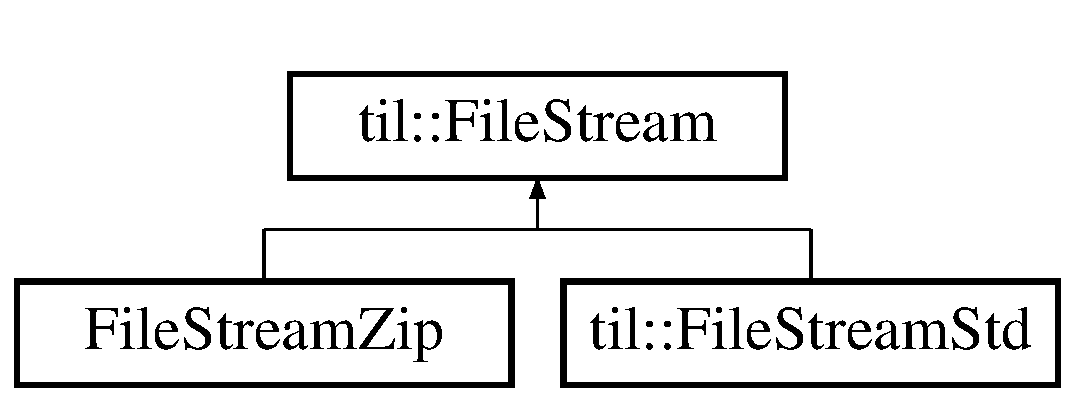
\includegraphics[height=2.000000cm]{classtil_1_1_file_stream}
\end{center}
\end{figure}
\subsection*{Public Member Functions}
\begin{DoxyCompactItemize}
\item 
virtual bool \hyperlink{classtil_1_1_file_stream_a907973c36daaa764e0b898540ffc24e8}{Open} (const char $\ast$a\_\-File, \hyperlink{namespacetil_a20db61688ed403d11f057a508d87e54c}{uint32} a\_\-Options)=0
\begin{DoxyCompactList}\small\item\em Open a handle to a file. \item\end{DoxyCompactList}\item 
virtual bool \hyperlink{classtil_1_1_file_stream_a26c0a9cc315418ab156ee3a56aad1be2}{Read} (void $\ast$a\_\-Dst, \hyperlink{namespacetil_a20db61688ed403d11f057a508d87e54c}{uint32} a\_\-ElementSize, \hyperlink{namespacetil_a20db61688ed403d11f057a508d87e54c}{uint32} a\_\-Count=1)=0
\begin{DoxyCompactList}\small\item\em Read data. \item\end{DoxyCompactList}\item 
virtual bool \hyperlink{classtil_1_1_file_stream_aeddef50dcb9b7353799800cccf942551}{ReadByte} (\hyperlink{namespacetil_a5f3ec10aca1a788b495a0bd3787bc2dc}{byte} $\ast$a\_\-Dst, \hyperlink{namespacetil_a20db61688ed403d11f057a508d87e54c}{uint32} a\_\-Count=1)=0
\begin{DoxyCompactList}\small\item\em Read a number of bytes. \item\end{DoxyCompactList}\item 
virtual bool \hyperlink{classtil_1_1_file_stream_aada6e2d7cd5fe720527b09da42f78222}{ReadWord} (\hyperlink{namespacetil_a7903a6761ac6f7472530b2863401909e}{word} $\ast$a\_\-Dst, \hyperlink{namespacetil_a20db61688ed403d11f057a508d87e54c}{uint32} a\_\-Count=1)=0
\begin{DoxyCompactList}\small\item\em Read a number of words. \item\end{DoxyCompactList}\item 
virtual bool \hyperlink{classtil_1_1_file_stream_a0a4a3add4a7fa4fd46e5ae4b38dbd9d3}{ReadDWord} (\hyperlink{namespacetil_a9babb870ec6cf9716ed0c90ea12811af}{dword} $\ast$a\_\-Dst, \hyperlink{namespacetil_a20db61688ed403d11f057a508d87e54c}{uint32} a\_\-Count=1)=0
\begin{DoxyCompactList}\small\item\em Read a number of dwords. \item\end{DoxyCompactList}\item 
virtual bool \hyperlink{classtil_1_1_file_stream_a29dfe625c988d68478ac6418478f7ea1}{Seek} (\hyperlink{namespacetil_a20db61688ed403d11f057a508d87e54c}{uint32} a\_\-Offset, \hyperlink{namespacetil_a20db61688ed403d11f057a508d87e54c}{uint32} a\_\-Options)=0
\begin{DoxyCompactList}\small\item\em Seek to a position in the file. \item\end{DoxyCompactList}\item 
virtual bool \hyperlink{classtil_1_1_file_stream_a693c2379367badd18d65d7f83512f595}{EndOfFile} ()=0
\begin{DoxyCompactList}\small\item\em Check for end of file. \item\end{DoxyCompactList}\item 
virtual bool \hyperlink{classtil_1_1_file_stream_a247dffc5fa0875cbafb48c63baa03493}{Close} ()=0
\begin{DoxyCompactList}\small\item\em Close the stream. \item\end{DoxyCompactList}\item 
char $\ast$ \hyperlink{classtil_1_1_file_stream_a11c2696a386b75cbcb3194a944debc78}{GetFilePath} ()
\begin{DoxyCompactList}\small\item\em Get the full path. \item\end{DoxyCompactList}\end{DoxyCompactItemize}
\subsection*{Protected Attributes}
\begin{DoxyCompactItemize}
\item 
\hypertarget{classtil_1_1_file_stream_ae96d56b6be09292181e4a6924e3fa2f1}{
char $\ast$ \hyperlink{classtil_1_1_file_stream_ae96d56b6be09292181e4a6924e3fa2f1}{m\_\-FilePath}}
\label{classtil_1_1_file_stream_ae96d56b6be09292181e4a6924e3fa2f1}

\begin{DoxyCompactList}\small\item\em The full path to the file. \item\end{DoxyCompactList}\end{DoxyCompactItemize}


\subsection{Detailed Description}
The virtual interface for reading data from files. Reads data from a file in bytes. Platform-\/specific implementations can be made by inheriting from this class and attaching a new FileStreamFunc to TinyImageLoader.


\begin{DoxyCode}
                FileStream* OpenStreamMyDevice(const char* a_Path, uint32 a_Optio
      ns)
                {
                        FileStream* result = new FileStreamMyDevice();
                        if (result->Open(a_Path, a_Options)) { return result; }

                        return NULL;
                }
\end{DoxyCode}
 

\subsection{Member Function Documentation}
\hypertarget{classtil_1_1_file_stream_a247dffc5fa0875cbafb48c63baa03493}{
\index{til::FileStream@{til::FileStream}!Close@{Close}}
\index{Close@{Close}!til::FileStream@{til::FileStream}}
\subsubsection[{Close}]{\setlength{\rightskip}{0pt plus 5cm}virtual bool til::FileStream::Close (
\begin{DoxyParamCaption}
{}
\end{DoxyParamCaption}
)\hspace{0.3cm}{\ttfamily  \mbox{[}pure virtual\mbox{]}}}}
\label{classtil_1_1_file_stream_a247dffc5fa0875cbafb48c63baa03493}


Close the stream. 

Close the handle to the file.

\begin{DoxyReturn}{Returns}
Success 
\end{DoxyReturn}


Implemented in \hyperlink{classtil_1_1_file_stream_std_a13ecdaa29a9d998a77059f2a732dbca0}{til::FileStreamStd}.

\hypertarget{classtil_1_1_file_stream_a693c2379367badd18d65d7f83512f595}{
\index{til::FileStream@{til::FileStream}!EndOfFile@{EndOfFile}}
\index{EndOfFile@{EndOfFile}!til::FileStream@{til::FileStream}}
\subsubsection[{EndOfFile}]{\setlength{\rightskip}{0pt plus 5cm}virtual bool til::FileStream::EndOfFile (
\begin{DoxyParamCaption}
{}
\end{DoxyParamCaption}
)\hspace{0.3cm}{\ttfamily  \mbox{[}pure virtual\mbox{]}}}}
\label{classtil_1_1_file_stream_a693c2379367badd18d65d7f83512f595}


Check for end of file. 

\begin{DoxyReturn}{Returns}
True if no more bytes can be read, otherwise false 
\end{DoxyReturn}


Implemented in \hyperlink{classtil_1_1_file_stream_std_afe96b90d15f23582412eb2a03e9af254}{til::FileStreamStd}.

\hypertarget{classtil_1_1_file_stream_a11c2696a386b75cbcb3194a944debc78}{
\index{til::FileStream@{til::FileStream}!GetFilePath@{GetFilePath}}
\index{GetFilePath@{GetFilePath}!til::FileStream@{til::FileStream}}
\subsubsection[{GetFilePath}]{\setlength{\rightskip}{0pt plus 5cm}char$\ast$ til::FileStream::GetFilePath (
\begin{DoxyParamCaption}
{}
\end{DoxyParamCaption}
)\hspace{0.3cm}{\ttfamily  \mbox{[}inline\mbox{]}}}}
\label{classtil_1_1_file_stream_a11c2696a386b75cbcb3194a944debc78}


Get the full path. 

\begin{DoxyNote}{Note}
This string should always end with an image file extension, otherwise TinyImageLoader can't load it.
\end{DoxyNote}
\begin{DoxyReturn}{Returns}
a string with the full path to the file 
\end{DoxyReturn}
\hypertarget{classtil_1_1_file_stream_a907973c36daaa764e0b898540ffc24e8}{
\index{til::FileStream@{til::FileStream}!Open@{Open}}
\index{Open@{Open}!til::FileStream@{til::FileStream}}
\subsubsection[{Open}]{\setlength{\rightskip}{0pt plus 5cm}virtual bool til::FileStream::Open (
\begin{DoxyParamCaption}
\item[{const char $\ast$}]{a\_\-File, }
\item[{{\bf uint32}}]{a\_\-Options}
\end{DoxyParamCaption}
)\hspace{0.3cm}{\ttfamily  \mbox{[}pure virtual\mbox{]}}}}
\label{classtil_1_1_file_stream_a907973c36daaa764e0b898540ffc24e8}


Open a handle to a file. 


\begin{DoxyParams}{Parameters}
{\em a\_\-File} & The path to the file to be loaded \\
\hline
{\em a\_\-Options} & The options to consider\\
\hline
\end{DoxyParams}
\begin{DoxyReturn}{Returns}
True on success, false on failure
\end{DoxyReturn}
Valid options are a file option:
\begin{DoxyItemize}
\item \hyperlink{_t_i_l_settings_8h_a35df91f5e83de2ea6177f37406e487d9}{TIL\_\-FILE\_\-ABSOLUTEPATH}
\item \hyperlink{_t_i_l_settings_8h_a46033ff709c68056a163fefecfae188a}{TIL\_\-FILE\_\-ADDWORKINGDIR}
\end{DoxyItemize}

\begin{DoxyNote}{Note}
If a file cannot be found, return false 
\end{DoxyNote}


Implemented in \hyperlink{classtil_1_1_file_stream_std_ab58f46883a8ccf5e3884fef0b6cb42d3}{til::FileStreamStd}.

\hypertarget{classtil_1_1_file_stream_a26c0a9cc315418ab156ee3a56aad1be2}{
\index{til::FileStream@{til::FileStream}!Read@{Read}}
\index{Read@{Read}!til::FileStream@{til::FileStream}}
\subsubsection[{Read}]{\setlength{\rightskip}{0pt plus 5cm}virtual bool til::FileStream::Read (
\begin{DoxyParamCaption}
\item[{void $\ast$}]{a\_\-Dst, }
\item[{{\bf uint32}}]{a\_\-ElementSize, }
\item[{{\bf uint32}}]{a\_\-Count = {\ttfamily 1}}
\end{DoxyParamCaption}
)\hspace{0.3cm}{\ttfamily  \mbox{[}pure virtual\mbox{]}}}}
\label{classtil_1_1_file_stream_a26c0a9cc315418ab156ee3a56aad1be2}


Read data. 


\begin{DoxyParams}{Parameters}
{\em a\_\-Dst} & The destination buffer to write to \\
\hline
{\em a\_\-ElementSize} & The size of each element \\
\hline
{\em a\_\-Count} & The number of elements to read\\
\hline
\end{DoxyParams}
\begin{DoxyReturn}{Returns}
True on success, false on failure
\end{DoxyReturn}
\begin{DoxyNote}{Note}
If more data is requested than is left in the file, return false 
\end{DoxyNote}


Implemented in \hyperlink{classtil_1_1_file_stream_std_a5a4b5bb51ab27c50f2276c7c904e31b4}{til::FileStreamStd}.

\hypertarget{classtil_1_1_file_stream_aeddef50dcb9b7353799800cccf942551}{
\index{til::FileStream@{til::FileStream}!ReadByte@{ReadByte}}
\index{ReadByte@{ReadByte}!til::FileStream@{til::FileStream}}
\subsubsection[{ReadByte}]{\setlength{\rightskip}{0pt plus 5cm}virtual bool til::FileStream::ReadByte (
\begin{DoxyParamCaption}
\item[{{\bf byte} $\ast$}]{a\_\-Dst, }
\item[{{\bf uint32}}]{a\_\-Count = {\ttfamily 1}}
\end{DoxyParamCaption}
)\hspace{0.3cm}{\ttfamily  \mbox{[}pure virtual\mbox{]}}}}
\label{classtil_1_1_file_stream_aeddef50dcb9b7353799800cccf942551}


Read a number of bytes. 


\begin{DoxyParams}{Parameters}
{\em a\_\-Dst} & The destination buffer to write to \\
\hline
{\em a\_\-Count} & The number of bytes to read\\
\hline
\end{DoxyParams}
\begin{DoxyReturn}{Returns}
True on success, false on failure
\end{DoxyReturn}
\begin{DoxyNote}{Note}
If more data is requested than is left in the file, return false 
\end{DoxyNote}


Implemented in \hyperlink{classtil_1_1_file_stream_std_a1eea3ea2ef520676df5f5b0c51c2659f}{til::FileStreamStd}.

\hypertarget{classtil_1_1_file_stream_a0a4a3add4a7fa4fd46e5ae4b38dbd9d3}{
\index{til::FileStream@{til::FileStream}!ReadDWord@{ReadDWord}}
\index{ReadDWord@{ReadDWord}!til::FileStream@{til::FileStream}}
\subsubsection[{ReadDWord}]{\setlength{\rightskip}{0pt plus 5cm}virtual bool til::FileStream::ReadDWord (
\begin{DoxyParamCaption}
\item[{{\bf dword} $\ast$}]{a\_\-Dst, }
\item[{{\bf uint32}}]{a\_\-Count = {\ttfamily 1}}
\end{DoxyParamCaption}
)\hspace{0.3cm}{\ttfamily  \mbox{[}pure virtual\mbox{]}}}}
\label{classtil_1_1_file_stream_a0a4a3add4a7fa4fd46e5ae4b38dbd9d3}


Read a number of dwords. 


\begin{DoxyParams}{Parameters}
{\em a\_\-Dst} & The destination buffer to write to \\
\hline
{\em a\_\-Count} & The number of dwords to read\\
\hline
\end{DoxyParams}
\begin{DoxyReturn}{Returns}
True on success, false on failure
\end{DoxyReturn}
\begin{DoxyNote}{Note}
If more data is requested than is left in the file, return false 
\end{DoxyNote}


Implemented in \hyperlink{classtil_1_1_file_stream_std_a638af52afa0f132221dea6cb5b79faa6}{til::FileStreamStd}.

\hypertarget{classtil_1_1_file_stream_aada6e2d7cd5fe720527b09da42f78222}{
\index{til::FileStream@{til::FileStream}!ReadWord@{ReadWord}}
\index{ReadWord@{ReadWord}!til::FileStream@{til::FileStream}}
\subsubsection[{ReadWord}]{\setlength{\rightskip}{0pt plus 5cm}virtual bool til::FileStream::ReadWord (
\begin{DoxyParamCaption}
\item[{{\bf word} $\ast$}]{a\_\-Dst, }
\item[{{\bf uint32}}]{a\_\-Count = {\ttfamily 1}}
\end{DoxyParamCaption}
)\hspace{0.3cm}{\ttfamily  \mbox{[}pure virtual\mbox{]}}}}
\label{classtil_1_1_file_stream_aada6e2d7cd5fe720527b09da42f78222}


Read a number of words. 


\begin{DoxyParams}{Parameters}
{\em a\_\-Dst} & The destination buffer to write to \\
\hline
{\em a\_\-Count} & The number of words to read\\
\hline
\end{DoxyParams}
\begin{DoxyReturn}{Returns}
True on success, false on failure
\end{DoxyReturn}
\begin{DoxyNote}{Note}
If more data is requested than is left in the file, return false 
\end{DoxyNote}


Implemented in \hyperlink{classtil_1_1_file_stream_std_aadd59b38678d22428f311aa417aeca40}{til::FileStreamStd}.

\hypertarget{classtil_1_1_file_stream_a29dfe625c988d68478ac6418478f7ea1}{
\index{til::FileStream@{til::FileStream}!Seek@{Seek}}
\index{Seek@{Seek}!til::FileStream@{til::FileStream}}
\subsubsection[{Seek}]{\setlength{\rightskip}{0pt plus 5cm}virtual bool til::FileStream::Seek (
\begin{DoxyParamCaption}
\item[{{\bf uint32}}]{a\_\-Offset, }
\item[{{\bf uint32}}]{a\_\-Options}
\end{DoxyParamCaption}
)\hspace{0.3cm}{\ttfamily  \mbox{[}pure virtual\mbox{]}}}}
\label{classtil_1_1_file_stream_a29dfe625c988d68478ac6418478f7ea1}


Seek to a position in the file. 


\begin{DoxyParams}{Parameters}
{\em a\_\-Offset} & The number of bytes to skip \\
\hline
{\em a\_\-Options} & The location in the file\\
\hline
\end{DoxyParams}
Valid options are: -\/\hyperlink{_t_i_l_settings_8h_a973d977edd49701c43cece50966e26a2}{TIL\_\-FILE\_\-SEEK\_\-START} -\/\hyperlink{_t_i_l_settings_8h_a5055479b805b9dfdd4383561c8ce0006}{TIL\_\-FILE\_\-SEEK\_\-CURR} -\/\hyperlink{_t_i_l_settings_8h_a56022a317f988fecf7ed712b02382378}{TIL\_\-FILE\_\-SEEK\_\-END}

\begin{DoxyReturn}{Returns}
True on success, false on failure
\end{DoxyReturn}
\begin{DoxyNote}{Note}
If the requested offset is too great, clamp to the nearest edge (either the start or the end of the file) and return false 
\end{DoxyNote}


Implemented in \hyperlink{classtil_1_1_file_stream_std_a8e3874550cefaec46846237a68c7727d}{til::FileStreamStd}.



The documentation for this class was generated from the following files:\begin{DoxyCompactItemize}
\item 
SDK/headers/\hyperlink{_t_i_l_file_stream_8h}{TILFileStream.h}\item 
src/TILFileStream.cpp\end{DoxyCompactItemize}

\hypertarget{classtil_1_1_file_stream_std}{
\section{til::FileStreamStd Class Reference}
\label{classtil_1_1_file_stream_std}\index{til::FileStreamStd@{til::FileStreamStd}}
}


ANSI C implementation of \hyperlink{classtil_1_1_file_stream}{FileStream}.  




{\ttfamily \#include $<$TILFileStreamStd.h$>$}

Inheritance diagram for til::FileStreamStd:\begin{figure}[H]
\begin{center}
\leavevmode
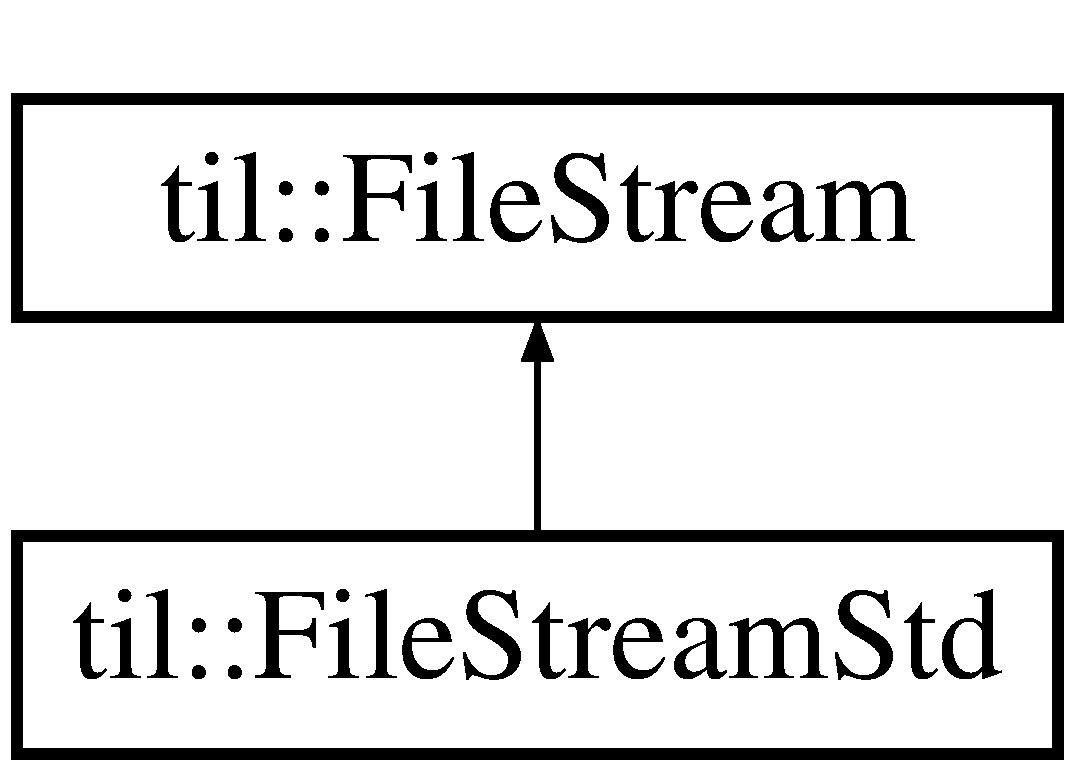
\includegraphics[height=2.000000cm]{classtil_1_1_file_stream_std}
\end{center}
\end{figure}
\subsection*{Public Member Functions}
\begin{DoxyCompactItemize}
\item 
bool \hyperlink{classtil_1_1_file_stream_std_ab58f46883a8ccf5e3884fef0b6cb42d3}{Open} (const char $\ast$a\_\-File, \hyperlink{namespacetil_a20db61688ed403d11f057a508d87e54c}{uint32} a\_\-Options)
\begin{DoxyCompactList}\small\item\em Open a handle to a file. \item\end{DoxyCompactList}\item 
bool \hyperlink{classtil_1_1_file_stream_std_a5a4b5bb51ab27c50f2276c7c904e31b4}{Read} (void $\ast$a\_\-Dst, \hyperlink{namespacetil_a20db61688ed403d11f057a508d87e54c}{uint32} a\_\-ElementSize, \hyperlink{namespacetil_a20db61688ed403d11f057a508d87e54c}{uint32} a\_\-Count=1)
\begin{DoxyCompactList}\small\item\em Read data. \item\end{DoxyCompactList}\item 
bool \hyperlink{classtil_1_1_file_stream_std_a1eea3ea2ef520676df5f5b0c51c2659f}{ReadByte} (\hyperlink{namespacetil_a5f3ec10aca1a788b495a0bd3787bc2dc}{byte} $\ast$a\_\-Dst, \hyperlink{namespacetil_a20db61688ed403d11f057a508d87e54c}{uint32} a\_\-Count=1)
\begin{DoxyCompactList}\small\item\em Read a number of bytes. \item\end{DoxyCompactList}\item 
bool \hyperlink{classtil_1_1_file_stream_std_aadd59b38678d22428f311aa417aeca40}{ReadWord} (\hyperlink{namespacetil_a7903a6761ac6f7472530b2863401909e}{word} $\ast$a\_\-Dst, \hyperlink{namespacetil_a20db61688ed403d11f057a508d87e54c}{uint32} a\_\-Count=1)
\begin{DoxyCompactList}\small\item\em Read a number of words. \item\end{DoxyCompactList}\item 
bool \hyperlink{classtil_1_1_file_stream_std_a638af52afa0f132221dea6cb5b79faa6}{ReadDWord} (\hyperlink{namespacetil_a9babb870ec6cf9716ed0c90ea12811af}{dword} $\ast$a\_\-Dst, \hyperlink{namespacetil_a20db61688ed403d11f057a508d87e54c}{uint32} a\_\-Count=1)
\begin{DoxyCompactList}\small\item\em Read a number of dwords. \item\end{DoxyCompactList}\item 
bool \hyperlink{classtil_1_1_file_stream_std_a8e3874550cefaec46846237a68c7727d}{Seek} (\hyperlink{namespacetil_a20db61688ed403d11f057a508d87e54c}{uint32} a\_\-Bytes, \hyperlink{namespacetil_a20db61688ed403d11f057a508d87e54c}{uint32} a\_\-Options)
\begin{DoxyCompactList}\small\item\em Seek to a position in the file. \item\end{DoxyCompactList}\item 
bool \hyperlink{classtil_1_1_file_stream_std_afe96b90d15f23582412eb2a03e9af254}{EndOfFile} ()
\begin{DoxyCompactList}\small\item\em Check for end of file. \item\end{DoxyCompactList}\item 
bool \hyperlink{classtil_1_1_file_stream_std_a13ecdaa29a9d998a77059f2a732dbca0}{Close} ()
\begin{DoxyCompactList}\small\item\em Close the stream. \item\end{DoxyCompactList}\end{DoxyCompactItemize}


\subsection{Detailed Description}
ANSI C implementation of \hyperlink{classtil_1_1_file_stream}{FileStream}. \hyperlink{classtil_1_1_file_stream}{FileStream} implementation that uses FILE pointers. Should work on all platforms with a valid ANSI C implementation, but details may differ. 

\subsection{Member Function Documentation}
\hypertarget{classtil_1_1_file_stream_std_a13ecdaa29a9d998a77059f2a732dbca0}{
\index{til::FileStreamStd@{til::FileStreamStd}!Close@{Close}}
\index{Close@{Close}!til::FileStreamStd@{til::FileStreamStd}}
\subsubsection[{Close}]{\setlength{\rightskip}{0pt plus 5cm}bool til::FileStreamStd::Close (
\begin{DoxyParamCaption}
{}
\end{DoxyParamCaption}
)\hspace{0.3cm}{\ttfamily  \mbox{[}virtual\mbox{]}}}}
\label{classtil_1_1_file_stream_std_a13ecdaa29a9d998a77059f2a732dbca0}


Close the stream. 

Close the handle to the file.

\begin{DoxyReturn}{Returns}
Success 
\end{DoxyReturn}


Implements \hyperlink{classtil_1_1_file_stream_a247dffc5fa0875cbafb48c63baa03493}{til::FileStream}.

\hypertarget{classtil_1_1_file_stream_std_afe96b90d15f23582412eb2a03e9af254}{
\index{til::FileStreamStd@{til::FileStreamStd}!EndOfFile@{EndOfFile}}
\index{EndOfFile@{EndOfFile}!til::FileStreamStd@{til::FileStreamStd}}
\subsubsection[{EndOfFile}]{\setlength{\rightskip}{0pt plus 5cm}bool til::FileStreamStd::EndOfFile (
\begin{DoxyParamCaption}
{}
\end{DoxyParamCaption}
)\hspace{0.3cm}{\ttfamily  \mbox{[}virtual\mbox{]}}}}
\label{classtil_1_1_file_stream_std_afe96b90d15f23582412eb2a03e9af254}


Check for end of file. 

\begin{DoxyReturn}{Returns}
True if no more bytes can be read, otherwise false 
\end{DoxyReturn}


Implements \hyperlink{classtil_1_1_file_stream_a693c2379367badd18d65d7f83512f595}{til::FileStream}.

\hypertarget{classtil_1_1_file_stream_std_ab58f46883a8ccf5e3884fef0b6cb42d3}{
\index{til::FileStreamStd@{til::FileStreamStd}!Open@{Open}}
\index{Open@{Open}!til::FileStreamStd@{til::FileStreamStd}}
\subsubsection[{Open}]{\setlength{\rightskip}{0pt plus 5cm}bool til::FileStreamStd::Open (
\begin{DoxyParamCaption}
\item[{const char $\ast$}]{a\_\-File, }
\item[{{\bf uint32}}]{a\_\-Options}
\end{DoxyParamCaption}
)\hspace{0.3cm}{\ttfamily  \mbox{[}virtual\mbox{]}}}}
\label{classtil_1_1_file_stream_std_ab58f46883a8ccf5e3884fef0b6cb42d3}


Open a handle to a file. 


\begin{DoxyParams}{Parameters}
{\em a\_\-File} & The path to the file to be loaded \\
\hline
{\em a\_\-Options} & The options to consider\\
\hline
\end{DoxyParams}
\begin{DoxyReturn}{Returns}
True on success, false on failure
\end{DoxyReturn}
Valid options are a file option:
\begin{DoxyItemize}
\item \hyperlink{_t_i_l_settings_8h_a35df91f5e83de2ea6177f37406e487d9}{TIL\_\-FILE\_\-ABSOLUTEPATH}
\item \hyperlink{_t_i_l_settings_8h_a46033ff709c68056a163fefecfae188a}{TIL\_\-FILE\_\-ADDWORKINGDIR}
\end{DoxyItemize}

\begin{DoxyNote}{Note}
If a file cannot be found, return false 
\end{DoxyNote}


Implements \hyperlink{classtil_1_1_file_stream_a907973c36daaa764e0b898540ffc24e8}{til::FileStream}.

\hypertarget{classtil_1_1_file_stream_std_a5a4b5bb51ab27c50f2276c7c904e31b4}{
\index{til::FileStreamStd@{til::FileStreamStd}!Read@{Read}}
\index{Read@{Read}!til::FileStreamStd@{til::FileStreamStd}}
\subsubsection[{Read}]{\setlength{\rightskip}{0pt plus 5cm}bool til::FileStreamStd::Read (
\begin{DoxyParamCaption}
\item[{void $\ast$}]{a\_\-Dst, }
\item[{{\bf uint32}}]{a\_\-ElementSize, }
\item[{{\bf uint32}}]{a\_\-Count = {\ttfamily 1}}
\end{DoxyParamCaption}
)\hspace{0.3cm}{\ttfamily  \mbox{[}virtual\mbox{]}}}}
\label{classtil_1_1_file_stream_std_a5a4b5bb51ab27c50f2276c7c904e31b4}


Read data. 


\begin{DoxyParams}{Parameters}
{\em a\_\-Dst} & The destination buffer to write to \\
\hline
{\em a\_\-ElementSize} & The size of each element \\
\hline
{\em a\_\-Count} & The number of elements to read\\
\hline
\end{DoxyParams}
\begin{DoxyReturn}{Returns}
True on success, false on failure
\end{DoxyReturn}
\begin{DoxyNote}{Note}
If more data is requested than is left in the file, return false 
\end{DoxyNote}


Implements \hyperlink{classtil_1_1_file_stream_a26c0a9cc315418ab156ee3a56aad1be2}{til::FileStream}.

\hypertarget{classtil_1_1_file_stream_std_a1eea3ea2ef520676df5f5b0c51c2659f}{
\index{til::FileStreamStd@{til::FileStreamStd}!ReadByte@{ReadByte}}
\index{ReadByte@{ReadByte}!til::FileStreamStd@{til::FileStreamStd}}
\subsubsection[{ReadByte}]{\setlength{\rightskip}{0pt plus 5cm}bool til::FileStreamStd::ReadByte (
\begin{DoxyParamCaption}
\item[{{\bf byte} $\ast$}]{a\_\-Dst, }
\item[{{\bf uint32}}]{a\_\-Count = {\ttfamily 1}}
\end{DoxyParamCaption}
)\hspace{0.3cm}{\ttfamily  \mbox{[}virtual\mbox{]}}}}
\label{classtil_1_1_file_stream_std_a1eea3ea2ef520676df5f5b0c51c2659f}


Read a number of bytes. 


\begin{DoxyParams}{Parameters}
{\em a\_\-Dst} & The destination buffer to write to \\
\hline
{\em a\_\-Count} & The number of bytes to read\\
\hline
\end{DoxyParams}
\begin{DoxyReturn}{Returns}
True on success, false on failure
\end{DoxyReturn}
\begin{DoxyNote}{Note}
If more data is requested than is left in the file, return false 
\end{DoxyNote}


Implements \hyperlink{classtil_1_1_file_stream_aeddef50dcb9b7353799800cccf942551}{til::FileStream}.

\hypertarget{classtil_1_1_file_stream_std_a638af52afa0f132221dea6cb5b79faa6}{
\index{til::FileStreamStd@{til::FileStreamStd}!ReadDWord@{ReadDWord}}
\index{ReadDWord@{ReadDWord}!til::FileStreamStd@{til::FileStreamStd}}
\subsubsection[{ReadDWord}]{\setlength{\rightskip}{0pt plus 5cm}bool til::FileStreamStd::ReadDWord (
\begin{DoxyParamCaption}
\item[{{\bf dword} $\ast$}]{a\_\-Dst, }
\item[{{\bf uint32}}]{a\_\-Count = {\ttfamily 1}}
\end{DoxyParamCaption}
)\hspace{0.3cm}{\ttfamily  \mbox{[}virtual\mbox{]}}}}
\label{classtil_1_1_file_stream_std_a638af52afa0f132221dea6cb5b79faa6}


Read a number of dwords. 


\begin{DoxyParams}{Parameters}
{\em a\_\-Dst} & The destination buffer to write to \\
\hline
{\em a\_\-Count} & The number of dwords to read\\
\hline
\end{DoxyParams}
\begin{DoxyReturn}{Returns}
True on success, false on failure
\end{DoxyReturn}
\begin{DoxyNote}{Note}
If more data is requested than is left in the file, return false 
\end{DoxyNote}


Implements \hyperlink{classtil_1_1_file_stream_a0a4a3add4a7fa4fd46e5ae4b38dbd9d3}{til::FileStream}.

\hypertarget{classtil_1_1_file_stream_std_aadd59b38678d22428f311aa417aeca40}{
\index{til::FileStreamStd@{til::FileStreamStd}!ReadWord@{ReadWord}}
\index{ReadWord@{ReadWord}!til::FileStreamStd@{til::FileStreamStd}}
\subsubsection[{ReadWord}]{\setlength{\rightskip}{0pt plus 5cm}bool til::FileStreamStd::ReadWord (
\begin{DoxyParamCaption}
\item[{{\bf word} $\ast$}]{a\_\-Dst, }
\item[{{\bf uint32}}]{a\_\-Count = {\ttfamily 1}}
\end{DoxyParamCaption}
)\hspace{0.3cm}{\ttfamily  \mbox{[}virtual\mbox{]}}}}
\label{classtil_1_1_file_stream_std_aadd59b38678d22428f311aa417aeca40}


Read a number of words. 


\begin{DoxyParams}{Parameters}
{\em a\_\-Dst} & The destination buffer to write to \\
\hline
{\em a\_\-Count} & The number of words to read\\
\hline
\end{DoxyParams}
\begin{DoxyReturn}{Returns}
True on success, false on failure
\end{DoxyReturn}
\begin{DoxyNote}{Note}
If more data is requested than is left in the file, return false 
\end{DoxyNote}


Implements \hyperlink{classtil_1_1_file_stream_aada6e2d7cd5fe720527b09da42f78222}{til::FileStream}.

\hypertarget{classtil_1_1_file_stream_std_a8e3874550cefaec46846237a68c7727d}{
\index{til::FileStreamStd@{til::FileStreamStd}!Seek@{Seek}}
\index{Seek@{Seek}!til::FileStreamStd@{til::FileStreamStd}}
\subsubsection[{Seek}]{\setlength{\rightskip}{0pt plus 5cm}bool til::FileStreamStd::Seek (
\begin{DoxyParamCaption}
\item[{{\bf uint32}}]{a\_\-Offset, }
\item[{{\bf uint32}}]{a\_\-Options}
\end{DoxyParamCaption}
)\hspace{0.3cm}{\ttfamily  \mbox{[}virtual\mbox{]}}}}
\label{classtil_1_1_file_stream_std_a8e3874550cefaec46846237a68c7727d}


Seek to a position in the file. 


\begin{DoxyParams}{Parameters}
{\em a\_\-Offset} & The number of bytes to skip \\
\hline
{\em a\_\-Options} & The location in the file\\
\hline
\end{DoxyParams}
Valid options are: -\/\hyperlink{_t_i_l_settings_8h_a973d977edd49701c43cece50966e26a2}{TIL\_\-FILE\_\-SEEK\_\-START} -\/\hyperlink{_t_i_l_settings_8h_a5055479b805b9dfdd4383561c8ce0006}{TIL\_\-FILE\_\-SEEK\_\-CURR} -\/\hyperlink{_t_i_l_settings_8h_a56022a317f988fecf7ed712b02382378}{TIL\_\-FILE\_\-SEEK\_\-END}

\begin{DoxyReturn}{Returns}
True on success, false on failure
\end{DoxyReturn}
\begin{DoxyNote}{Note}
If the requested offset is too great, clamp to the nearest edge (either the start or the end of the file) and return false 
\end{DoxyNote}


Implements \hyperlink{classtil_1_1_file_stream_a29dfe625c988d68478ac6418478f7ea1}{til::FileStream}.



The documentation for this class was generated from the following files:\begin{DoxyCompactItemize}
\item 
SDK/headers/\hyperlink{_t_i_l_file_stream_std_8h}{TILFileStreamStd.h}\item 
src/TILFileStreamStd.cpp\end{DoxyCompactItemize}

\hypertarget{class_t_i_l_f_w_1_1_framework}{
\section{TILFW::Framework Class Reference}
\label{class_t_i_l_f_w_1_1_framework}\index{TILFW::Framework@{TILFW::Framework}}
}
\subsection*{Public Member Functions}
\begin{DoxyCompactItemize}
\item 
\hypertarget{class_t_i_l_f_w_1_1_framework_ae741a615824b09b039531c1ecd0c4ebe}{
int \hyperlink{class_t_i_l_f_w_1_1_framework_ae741a615824b09b039531c1ecd0c4ebe}{Exec} (HINSTANCE hInstance, HINSTANCE hPrevInstance, LPSTR lpCmdLine, int nCmdShow)}
\label{class_t_i_l_f_w_1_1_framework_ae741a615824b09b039531c1ecd0c4ebe}

\begin{DoxyCompactList}\small\item\em Main entry point for the examples. \item\end{DoxyCompactList}\item 
void \hyperlink{class_t_i_l_f_w_1_1_framework_a2416aef2383b7d879a9c249b1a303641}{Setup} ()
\begin{DoxyCompactList}\small\item\em Setting up parameters. \item\end{DoxyCompactList}\item 
\hypertarget{class_t_i_l_f_w_1_1_framework_a35b3f67924bad5512ed4e279f1ad91aa}{
void \hyperlink{class_t_i_l_f_w_1_1_framework_a35b3f67924bad5512ed4e279f1ad91aa}{Init} (const char $\ast$$\ast$a\_\-CommandLine, int a\_\-Commands)}
\label{class_t_i_l_f_w_1_1_framework_a35b3f67924bad5512ed4e279f1ad91aa}

\begin{DoxyCompactList}\small\item\em Initializing. \item\end{DoxyCompactList}\item 
\hypertarget{class_t_i_l_f_w_1_1_framework_a42420a83c470902e957af36baddd53ee}{
void \hyperlink{class_t_i_l_f_w_1_1_framework_a42420a83c470902e957af36baddd53ee}{Tick} (float a\_\-DT)}
\label{class_t_i_l_f_w_1_1_framework_a42420a83c470902e957af36baddd53ee}

\begin{DoxyCompactList}\small\item\em Main loop. \item\end{DoxyCompactList}\item 
\hypertarget{class_t_i_l_f_w_1_1_framework_ad780d90fcb7a69545efbe320dc12b726}{
void \hyperlink{class_t_i_l_f_w_1_1_framework_ad780d90fcb7a69545efbe320dc12b726}{Render} ()}
\label{class_t_i_l_f_w_1_1_framework_ad780d90fcb7a69545efbe320dc12b726}

\begin{DoxyCompactList}\small\item\em Rendering. \item\end{DoxyCompactList}\end{DoxyCompactItemize}
\subsection*{Public Attributes}
\begin{DoxyCompactItemize}
\item 
\hypertarget{class_t_i_l_f_w_1_1_framework_acc2823b02dfe5b7fb775a7e5db3415d3}{
unsigned int \hyperlink{class_t_i_l_f_w_1_1_framework_acc2823b02dfe5b7fb775a7e5db3415d3}{s\_\-WindowWidth}}
\label{class_t_i_l_f_w_1_1_framework_acc2823b02dfe5b7fb775a7e5db3415d3}

\begin{DoxyCompactList}\small\item\em Width of the window. \item\end{DoxyCompactList}\item 
\hypertarget{class_t_i_l_f_w_1_1_framework_af9e746ade44702026071be1ab910e90c}{
unsigned int \hyperlink{class_t_i_l_f_w_1_1_framework_af9e746ade44702026071be1ab910e90c}{s\_\-WindowHeight}}
\label{class_t_i_l_f_w_1_1_framework_af9e746ade44702026071be1ab910e90c}

\begin{DoxyCompactList}\small\item\em Height of the window. \item\end{DoxyCompactList}\item 
\hypertarget{class_t_i_l_f_w_1_1_framework_ad1b40fc088d50793b36eebe40eee12b7}{
bool \hyperlink{class_t_i_l_f_w_1_1_framework_ad1b40fc088d50793b36eebe40eee12b7}{s\_\-Exit}}
\label{class_t_i_l_f_w_1_1_framework_ad1b40fc088d50793b36eebe40eee12b7}

\begin{DoxyCompactList}\small\item\em Exits the program if true. \item\end{DoxyCompactList}\end{DoxyCompactItemize}
\subsection*{Static Public Attributes}
\begin{DoxyCompactItemize}
\item 
\hypertarget{class_t_i_l_f_w_1_1_framework_a36e2f073c0d10ce62ee0baf813b60d00}{
static bool \hyperlink{class_t_i_l_f_w_1_1_framework_a36e2f073c0d10ce62ee0baf813b60d00}{s\_\-KeysPressed} \mbox{[}256\mbox{]}}
\label{class_t_i_l_f_w_1_1_framework_a36e2f073c0d10ce62ee0baf813b60d00}

\begin{DoxyCompactList}\small\item\em List of keys held down. \item\end{DoxyCompactList}\item 
\hypertarget{class_t_i_l_f_w_1_1_framework_a64f626069888ea204f062e746b5deff2}{
static bool \hyperlink{class_t_i_l_f_w_1_1_framework_a64f626069888ea204f062e746b5deff2}{s\_\-KeysReleased} \mbox{[}256\mbox{]}}
\label{class_t_i_l_f_w_1_1_framework_a64f626069888ea204f062e746b5deff2}

\begin{DoxyCompactList}\small\item\em List of keys released in the last frame. \item\end{DoxyCompactList}\end{DoxyCompactItemize}


\subsection{Member Function Documentation}
\hypertarget{class_t_i_l_f_w_1_1_framework_a2416aef2383b7d879a9c249b1a303641}{
\index{TILFW::Framework@{TILFW::Framework}!Setup@{Setup}}
\index{Setup@{Setup}!TILFW::Framework@{TILFW::Framework}}
\subsubsection[{Setup}]{\setlength{\rightskip}{0pt plus 5cm}void TILFW::Framework::Setup (
\begin{DoxyParamCaption}
{}
\end{DoxyParamCaption}
)}}
\label{class_t_i_l_f_w_1_1_framework_a2416aef2383b7d879a9c249b1a303641}


Setting up parameters. 

Setting up some stuff. 

The documentation for this class was generated from the following files:\begin{DoxyCompactItemize}
\item 
examples/src/\hyperlink{_framework_8h}{Framework.h}\item 
examples/src/\hyperlink{example-opengl-texture_8cpp}{example-\/opengl-\/texture.cpp}\item 
examples/src/example-\/tests.cpp\item 
examples/src/\hyperlink{example-zip-loading_8cpp}{example-\/zip-\/loading.cpp}\item 
examples/src/Framework.cpp\end{DoxyCompactItemize}

\hypertarget{classtil_1_1_image}{
\section{til::Image Class Reference}
\label{classtil_1_1_image}\index{til::Image@{til::Image}}
}


The virtual interface for loading images and extracting image data.  




{\ttfamily \#include $<$TILImage.h$>$}

Inheritance diagram for til::Image:\begin{figure}[H]
\begin{center}
\leavevmode
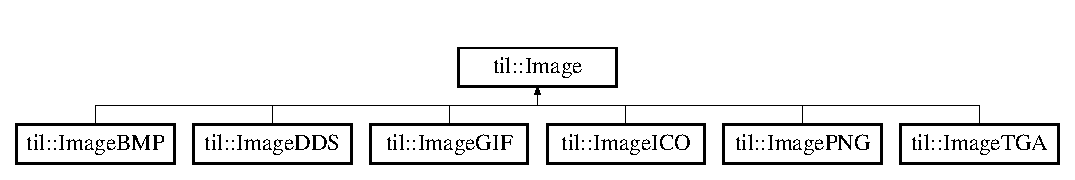
\includegraphics[height=1.964912cm]{classtil_1_1_image}
\end{center}
\end{figure}
\subsection*{Public Types}
\begin{DoxyCompactItemize}
\item 
enum \hyperlink{classtil_1_1_image_a621d337ba744563ed6bde962e08dfbc8}{BitDepth} \{ \par
\hyperlink{classtil_1_1_image_a621d337ba744563ed6bde962e08dfbc8af30c364fa646b255faed30d3a88564b6}{BPP\_\-32B\_\-A8R8G8B8} =  1, 
\hyperlink{classtil_1_1_image_a621d337ba744563ed6bde962e08dfbc8a0bf2ec10c9eed201fbfb41b5cf89b961}{BPP\_\-32B\_\-A8B8G8R8} =  2, 
\hyperlink{classtil_1_1_image_a621d337ba744563ed6bde962e08dfbc8a3ac84308671afc5f9063539355b916c9}{BPP\_\-32B\_\-R8G8B8A8} =  3, 
\hyperlink{classtil_1_1_image_a621d337ba744563ed6bde962e08dfbc8a0b77d25be4ba6617960ca436bd903fa8}{BPP\_\-32B\_\-B8G8R8A8} =  4, 
\par
\hyperlink{classtil_1_1_image_a621d337ba744563ed6bde962e08dfbc8a532664ea0fc09594fb9bddc0bed83120}{BPP\_\-32B\_\-R8G8B8} =  5, 
\hyperlink{classtil_1_1_image_a621d337ba744563ed6bde962e08dfbc8a328e608bddb9f328bf0bd1eae3e54b34}{BPP\_\-32B\_\-B8G8R8} =  6, 
\hyperlink{classtil_1_1_image_a621d337ba744563ed6bde962e08dfbc8aaa9732c2665f568a7fcea882b7b50a7d}{BPP\_\-16B\_\-R5G6B5} =  7, 
\hyperlink{classtil_1_1_image_a621d337ba744563ed6bde962e08dfbc8a8fff22180693d8663db79d0fbc290cac}{BPP\_\-16B\_\-B5G6R5} =  8
 \}
\begin{DoxyCompactList}\small\item\em The amount of bits per pixel and its arrangement. \item\end{DoxyCompactList}\end{DoxyCompactItemize}
\subsection*{Public Member Functions}
\begin{DoxyCompactItemize}
\item 
bool \hyperlink{classtil_1_1_image_ae1202f84c0addb81eba161f746a9d4cc}{SetBPP} (\hyperlink{namespacetil_a20db61688ed403d11f057a508d87e54c}{uint32} a\_\-Options)
\begin{DoxyCompactList}\small\item\em Sets the bit depth to convert to when parsing. \item\end{DoxyCompactList}\item 
\hypertarget{classtil_1_1_image_a33311ad048e924086afffabe7a21029d}{
\hyperlink{classtil_1_1_image_a621d337ba744563ed6bde962e08dfbc8}{BitDepth} \hyperlink{classtil_1_1_image_a33311ad048e924086afffabe7a21029d}{GetBitDepth} ()}
\label{classtil_1_1_image_a33311ad048e924086afffabe7a21029d}

\begin{DoxyCompactList}\small\item\em Get the color depth as an enum. \item\end{DoxyCompactList}\item 
void \hyperlink{classtil_1_1_image_aa8747fd600bc321cc0f2bea514a7d98b}{Load} (\hyperlink{classtil_1_1_file_stream}{FileStream} $\ast$a\_\-Stream)
\begin{DoxyCompactList}\small\item\em Load an image. \item\end{DoxyCompactList}\item 
bool \hyperlink{classtil_1_1_image_af6de495e7e1bea909e38b4eb1d1114e0}{Close} ()
\begin{DoxyCompactList}\small\item\em Closes the handle to the image file. \item\end{DoxyCompactList}\item 
virtual bool \hyperlink{classtil_1_1_image_a2436c982f6b403ab07591f06107fe432}{Parse} (\hyperlink{namespacetil_a20db61688ed403d11f057a508d87e54c}{uint32} a\_\-ColorDepth)=0
\begin{DoxyCompactList}\small\item\em Parses the actual image data. \item\end{DoxyCompactList}\item 
virtual \hyperlink{namespacetil_a20db61688ed403d11f057a508d87e54c}{uint32} \hyperlink{classtil_1_1_image_a78c10e07b535c99840b0afd5aa165df4}{GetFrameCount} ()
\begin{DoxyCompactList}\small\item\em Returns the amount of frames this image contains. \item\end{DoxyCompactList}\item 
virtual float \hyperlink{classtil_1_1_image_aabddc7f03e3d1962f5abb21c200f2050}{GetDelay} ()
\begin{DoxyCompactList}\small\item\em Returns the delay between frames. \item\end{DoxyCompactList}\item 
virtual \hyperlink{namespacetil_a5f3ec10aca1a788b495a0bd3787bc2dc}{byte} $\ast$ \hyperlink{classtil_1_1_image_a8dd46f6477025e23dc921e1a4a3f6a62}{GetPixels} (\hyperlink{namespacetil_a20db61688ed403d11f057a508d87e54c}{uint32} a\_\-Frame=0)=0
\begin{DoxyCompactList}\small\item\em Get the pixel data from this image. \item\end{DoxyCompactList}\item 
virtual \hyperlink{namespacetil_a20db61688ed403d11f057a508d87e54c}{uint32} \hyperlink{classtil_1_1_image_a769be7e5a2cc490e8ae70b7c29a56eca}{GetWidth} (\hyperlink{namespacetil_a20db61688ed403d11f057a508d87e54c}{uint32} a\_\-Frame=0)=0
\begin{DoxyCompactList}\small\item\em Get the width of a frame. \item\end{DoxyCompactList}\item 
virtual \hyperlink{namespacetil_a20db61688ed403d11f057a508d87e54c}{uint32} \hyperlink{classtil_1_1_image_ad623add911ba5230f56a4cc58af75ec1}{GetHeight} (\hyperlink{namespacetil_a20db61688ed403d11f057a508d87e54c}{uint32} a\_\-Frame=0)=0
\begin{DoxyCompactList}\small\item\em Get the height of a frame. \item\end{DoxyCompactList}\end{DoxyCompactItemize}
\subsection*{Protected Attributes}
\begin{DoxyCompactItemize}
\item 
\hypertarget{classtil_1_1_image_a99fcde28d6287cbf55b1a6307788f5c6}{
\hyperlink{classtil_1_1_file_stream}{FileStream} $\ast$ \hyperlink{classtil_1_1_image_a99fcde28d6287cbf55b1a6307788f5c6}{m\_\-Stream}}
\label{classtil_1_1_image_a99fcde28d6287cbf55b1a6307788f5c6}

\begin{DoxyCompactList}\small\item\em The file interface. \item\end{DoxyCompactList}\item 
\hypertarget{classtil_1_1_image_ac995efac9fe1641e276452bdb90fbddd}{
char $\ast$ \hyperlink{classtil_1_1_image_ac995efac9fe1641e276452bdb90fbddd}{m\_\-FileName}}
\label{classtil_1_1_image_ac995efac9fe1641e276452bdb90fbddd}

\begin{DoxyCompactList}\small\item\em The filename. \item\end{DoxyCompactList}\item 
\hypertarget{classtil_1_1_image_a200eeebc45a71c0935aee4e5afded433}{
\hyperlink{classtil_1_1_image_a621d337ba744563ed6bde962e08dfbc8}{BitDepth} \hyperlink{classtil_1_1_image_a200eeebc45a71c0935aee4e5afded433}{m\_\-BPPIdent}}
\label{classtil_1_1_image_a200eeebc45a71c0935aee4e5afded433}

\begin{DoxyCompactList}\small\item\em The bit depth to convert to. \item\end{DoxyCompactList}\item 
\hypertarget{classtil_1_1_image_af3aa350823454079c3bf84f30bcfd0c5}{
\hyperlink{namespacetil_a7a75b0e7e2cd3f19ea51c8c02fd242f8}{uint8} \hyperlink{classtil_1_1_image_af3aa350823454079c3bf84f30bcfd0c5}{m\_\-BPP}}
\label{classtil_1_1_image_af3aa350823454079c3bf84f30bcfd0c5}

\begin{DoxyCompactList}\small\item\em The amount of bytes per pixel. \item\end{DoxyCompactList}\end{DoxyCompactItemize}


\subsection{Detailed Description}
The virtual interface for loading images and extracting image data. All image operations go through this interface. Every image loader is an implementation of this class.

\subsection{Member Enumeration Documentation}
\hypertarget{classtil_1_1_image_a621d337ba744563ed6bde962e08dfbc8}{
\index{til::Image@{til::Image}!BitDepth@{BitDepth}}
\index{BitDepth@{BitDepth}!til::Image@{til::Image}}
\subsubsection[{BitDepth}]{\setlength{\rightskip}{0pt plus 5cm}enum {\bf til::Image::BitDepth}}}
\label{classtil_1_1_image_a621d337ba744563ed6bde962e08dfbc8}


The amount of bits per pixel and its arrangement. 

\begin{Desc}
\item[Enumerator: ]\par
\begin{description}
\index{BPP\_\-32B\_\-A8R8G8B8@{BPP\_\-32B\_\-A8R8G8B8}!til::Image@{til::Image}}\index{til::Image@{til::Image}!BPP\_\-32B\_\-A8R8G8B8@{BPP\_\-32B\_\-A8R8G8B8}}\item[{\em 
\hypertarget{classtil_1_1_image_a621d337ba744563ed6bde962e08dfbc8af30c364fa646b255faed30d3a88564b6}{
BPP\_\-32B\_\-A8R8G8B8}
\label{classtil_1_1_image_a621d337ba744563ed6bde962e08dfbc8af30c364fa646b255faed30d3a88564b6}
}]32-\/bit ARGB color \index{BPP\_\-32B\_\-A8B8G8R8@{BPP\_\-32B\_\-A8B8G8R8}!til::Image@{til::Image}}\index{til::Image@{til::Image}!BPP\_\-32B\_\-A8B8G8R8@{BPP\_\-32B\_\-A8B8G8R8}}\item[{\em 
\hypertarget{classtil_1_1_image_a621d337ba744563ed6bde962e08dfbc8a0bf2ec10c9eed201fbfb41b5cf89b961}{
BPP\_\-32B\_\-A8B8G8R8}
\label{classtil_1_1_image_a621d337ba744563ed6bde962e08dfbc8a0bf2ec10c9eed201fbfb41b5cf89b961}
}]32-\/bit ABGR color \index{BPP\_\-32B\_\-R8G8B8A8@{BPP\_\-32B\_\-R8G8B8A8}!til::Image@{til::Image}}\index{til::Image@{til::Image}!BPP\_\-32B\_\-R8G8B8A8@{BPP\_\-32B\_\-R8G8B8A8}}\item[{\em 
\hypertarget{classtil_1_1_image_a621d337ba744563ed6bde962e08dfbc8a3ac84308671afc5f9063539355b916c9}{
BPP\_\-32B\_\-R8G8B8A8}
\label{classtil_1_1_image_a621d337ba744563ed6bde962e08dfbc8a3ac84308671afc5f9063539355b916c9}
}]32-\/bit RGBA color \index{BPP\_\-32B\_\-B8G8R8A8@{BPP\_\-32B\_\-B8G8R8A8}!til::Image@{til::Image}}\index{til::Image@{til::Image}!BPP\_\-32B\_\-B8G8R8A8@{BPP\_\-32B\_\-B8G8R8A8}}\item[{\em 
\hypertarget{classtil_1_1_image_a621d337ba744563ed6bde962e08dfbc8a0b77d25be4ba6617960ca436bd903fa8}{
BPP\_\-32B\_\-B8G8R8A8}
\label{classtil_1_1_image_a621d337ba744563ed6bde962e08dfbc8a0b77d25be4ba6617960ca436bd903fa8}
}]32-\/bit BGRA color \index{BPP\_\-32B\_\-R8G8B8@{BPP\_\-32B\_\-R8G8B8}!til::Image@{til::Image}}\index{til::Image@{til::Image}!BPP\_\-32B\_\-R8G8B8@{BPP\_\-32B\_\-R8G8B8}}\item[{\em 
\hypertarget{classtil_1_1_image_a621d337ba744563ed6bde962e08dfbc8a532664ea0fc09594fb9bddc0bed83120}{
BPP\_\-32B\_\-R8G8B8}
\label{classtil_1_1_image_a621d337ba744563ed6bde962e08dfbc8a532664ea0fc09594fb9bddc0bed83120}
}]32-\/bit RGB color \index{BPP\_\-32B\_\-B8G8R8@{BPP\_\-32B\_\-B8G8R8}!til::Image@{til::Image}}\index{til::Image@{til::Image}!BPP\_\-32B\_\-B8G8R8@{BPP\_\-32B\_\-B8G8R8}}\item[{\em 
\hypertarget{classtil_1_1_image_a621d337ba744563ed6bde962e08dfbc8a328e608bddb9f328bf0bd1eae3e54b34}{
BPP\_\-32B\_\-B8G8R8}
\label{classtil_1_1_image_a621d337ba744563ed6bde962e08dfbc8a328e608bddb9f328bf0bd1eae3e54b34}
}]32-\/bit BGR color \index{BPP\_\-16B\_\-R5G6B5@{BPP\_\-16B\_\-R5G6B5}!til::Image@{til::Image}}\index{til::Image@{til::Image}!BPP\_\-16B\_\-R5G6B5@{BPP\_\-16B\_\-R5G6B5}}\item[{\em 
\hypertarget{classtil_1_1_image_a621d337ba744563ed6bde962e08dfbc8aaa9732c2665f568a7fcea882b7b50a7d}{
BPP\_\-16B\_\-R5G6B5}
\label{classtil_1_1_image_a621d337ba744563ed6bde962e08dfbc8aaa9732c2665f568a7fcea882b7b50a7d}
}]16-\/bit RGB color \index{BPP\_\-16B\_\-B5G6R5@{BPP\_\-16B\_\-B5G6R5}!til::Image@{til::Image}}\index{til::Image@{til::Image}!BPP\_\-16B\_\-B5G6R5@{BPP\_\-16B\_\-B5G6R5}}\item[{\em 
\hypertarget{classtil_1_1_image_a621d337ba744563ed6bde962e08dfbc8a8fff22180693d8663db79d0fbc290cac}{
BPP\_\-16B\_\-B5G6R5}
\label{classtil_1_1_image_a621d337ba744563ed6bde962e08dfbc8a8fff22180693d8663db79d0fbc290cac}
}]16-\/bit BGR color \end{description}
\end{Desc}



\subsection{Member Function Documentation}
\hypertarget{classtil_1_1_image_af6de495e7e1bea909e38b4eb1d1114e0}{
\index{til::Image@{til::Image}!Close@{Close}}
\index{Close@{Close}!til::Image@{til::Image}}
\subsubsection[{Close}]{\setlength{\rightskip}{0pt plus 5cm}bool til::Image::Close (
\begin{DoxyParamCaption}
{}
\end{DoxyParamCaption}
)}}
\label{classtil_1_1_image_af6de495e7e1bea909e38b4eb1d1114e0}


Closes the handle to the image file. 

Used internally by TinyImageLoader. \hypertarget{classtil_1_1_image_aabddc7f03e3d1962f5abb21c200f2050}{
\index{til::Image@{til::Image}!GetDelay@{GetDelay}}
\index{GetDelay@{GetDelay}!til::Image@{til::Image}}
\subsubsection[{GetDelay}]{\setlength{\rightskip}{0pt plus 5cm}virtual float til::Image::GetDelay (
\begin{DoxyParamCaption}
{}
\end{DoxyParamCaption}
)\hspace{0.3cm}{\ttfamily  \mbox{[}inline, virtual\mbox{]}}}}
\label{classtil_1_1_image_aabddc7f03e3d1962f5abb21c200f2050}


Returns the delay between frames. 

\begin{DoxyReturn}{Returns}
The delay in seconds between frames
\end{DoxyReturn}
Used when dealing with formats that support animation. 

Reimplemented in \hyperlink{classtil_1_1_image_g_i_f_a01af14634200dbb109d124746764d05d}{til::ImageGIF}.

\hypertarget{classtil_1_1_image_a78c10e07b535c99840b0afd5aa165df4}{
\index{til::Image@{til::Image}!GetFrameCount@{GetFrameCount}}
\index{GetFrameCount@{GetFrameCount}!til::Image@{til::Image}}
\subsubsection[{GetFrameCount}]{\setlength{\rightskip}{0pt plus 5cm}virtual {\bf uint32} til::Image::GetFrameCount (
\begin{DoxyParamCaption}
{}
\end{DoxyParamCaption}
)\hspace{0.3cm}{\ttfamily  \mbox{[}inline, virtual\mbox{]}}}}
\label{classtil_1_1_image_a78c10e07b535c99840b0afd5aa165df4}


Returns the amount of frames this image contains. 

Used when dealing with formats that support animation or multiple images.

\begin{DoxyNote}{Note}
There is never going to be support for other video formats. This is because TinyImageLoader is an $\ast$image$\ast$ loader, not a video loader. The exception to the rule are GIF89 and APNG, because it concerns an extension to a normally single-\/framed format. 
\end{DoxyNote}


Reimplemented in \hyperlink{classtil_1_1_image_b_m_p_a8a3a00823903dfd0e3b83b5b499d88f7}{til::ImageBMP}, \hyperlink{classtil_1_1_image_d_d_s_a616b077809ea2a4ebde9fa53651c198a}{til::ImageDDS}, \hyperlink{classtil_1_1_image_g_i_f_a9e0c056b0263196d305c9102f254240e}{til::ImageGIF}, \hyperlink{classtil_1_1_image_i_c_o_a58280b473d5ebc9864ade082f2f0f96d}{til::ImageICO}, \hyperlink{classtil_1_1_image_p_n_g_ade57a800697abe8f024a305e236b3471}{til::ImagePNG}, and \hyperlink{classtil_1_1_image_t_g_a_a46d1df102d6125290c6bba65a3ed9814}{til::ImageTGA}.

\hypertarget{classtil_1_1_image_ad623add911ba5230f56a4cc58af75ec1}{
\index{til::Image@{til::Image}!GetHeight@{GetHeight}}
\index{GetHeight@{GetHeight}!til::Image@{til::Image}}
\subsubsection[{GetHeight}]{\setlength{\rightskip}{0pt plus 5cm}virtual {\bf uint32} til::Image::GetHeight (
\begin{DoxyParamCaption}
\item[{{\bf uint32}}]{a\_\-Frame = {\ttfamily 0}}
\end{DoxyParamCaption}
)\hspace{0.3cm}{\ttfamily  \mbox{[}pure virtual\mbox{]}}}}
\label{classtil_1_1_image_ad623add911ba5230f56a4cc58af75ec1}


Get the height of a frame. 


\begin{DoxyParams}{Parameters}
{\em a\_\-Frame} & The frame of an animation or image to return.\\
\hline
\end{DoxyParams}
\begin{DoxyReturn}{Returns}
The height as a uint32.
\end{DoxyReturn}
Some formats support multiple frames or images with different dimensions. You can call this function with a frame number to get the correct dimensions. 

Implemented in \hyperlink{classtil_1_1_image_b_m_p_a9f6236bf4b43264f9b729a83a850a62b}{til::ImageBMP}, \hyperlink{classtil_1_1_image_d_d_s_a9ae6dc6b71a3a056eecd8b756d9089e8}{til::ImageDDS}, \hyperlink{classtil_1_1_image_g_i_f_ac241e6cacaf14d1e73aae50f105450ae}{til::ImageGIF}, \hyperlink{classtil_1_1_image_i_c_o_a9ae2f5e5d594f8b0a17690d72496605e}{til::ImageICO}, \hyperlink{classtil_1_1_image_p_n_g_a64dff92207203a4673290a0ed3634538}{til::ImagePNG}, and \hyperlink{classtil_1_1_image_t_g_a_a4284b8576ce42b239beec36bd6902eac}{til::ImageTGA}.

\hypertarget{classtil_1_1_image_a8dd46f6477025e23dc921e1a4a3f6a62}{
\index{til::Image@{til::Image}!GetPixels@{GetPixels}}
\index{GetPixels@{GetPixels}!til::Image@{til::Image}}
\subsubsection[{GetPixels}]{\setlength{\rightskip}{0pt plus 5cm}virtual {\bf byte}$\ast$ til::Image::GetPixels (
\begin{DoxyParamCaption}
\item[{{\bf uint32}}]{a\_\-Frame = {\ttfamily 0}}
\end{DoxyParamCaption}
)\hspace{0.3cm}{\ttfamily  \mbox{[}pure virtual\mbox{]}}}}
\label{classtil_1_1_image_a8dd46f6477025e23dc921e1a4a3f6a62}


Get the pixel data from this image. 


\begin{DoxyParams}{Parameters}
{\em a\_\-Frame} & The frame of an animation to return.\\
\hline
\end{DoxyParams}
\begin{DoxyReturn}{Returns}
Pixel array as a byte array.
\end{DoxyReturn}
The data is encoded according to the color depth specified. For instance, when loading images as 32-\/bit ARGB, the stream of bytes must be converted to unsigned long before being used.


\begin{DoxyCode}
                        til::Image* load = TIL_Load("media\\texture.png", 
      TIL_DEPTH_A8B8G8R8 | TIL_FILE_ADDWORKINGDIR);
                        unsigned long* pixels = (unsigned long*)load->GetPixels()
      ;
\end{DoxyCode}
 

Implemented in \hyperlink{classtil_1_1_image_b_m_p_a2a667c1f36e310f0040bfabc36fad6ba}{til::ImageBMP}, \hyperlink{classtil_1_1_image_d_d_s_ac14aad199b3430d527610f38498faa9e}{til::ImageDDS}, \hyperlink{classtil_1_1_image_g_i_f_ad9ee66121f0d4fe3a58af75177bb9245}{til::ImageGIF}, \hyperlink{classtil_1_1_image_i_c_o_a3501ed7aec07ea553855aff7cb58d7e8}{til::ImageICO}, \hyperlink{classtil_1_1_image_p_n_g_a2dc5b02cc0e64d2cf44202122c3e7e86}{til::ImagePNG}, and \hyperlink{classtil_1_1_image_t_g_a_a5202d714441c2df497368905bd4c5b83}{til::ImageTGA}.

\hypertarget{classtil_1_1_image_a769be7e5a2cc490e8ae70b7c29a56eca}{
\index{til::Image@{til::Image}!GetWidth@{GetWidth}}
\index{GetWidth@{GetWidth}!til::Image@{til::Image}}
\subsubsection[{GetWidth}]{\setlength{\rightskip}{0pt plus 5cm}virtual {\bf uint32} til::Image::GetWidth (
\begin{DoxyParamCaption}
\item[{{\bf uint32}}]{a\_\-Frame = {\ttfamily 0}}
\end{DoxyParamCaption}
)\hspace{0.3cm}{\ttfamily  \mbox{[}pure virtual\mbox{]}}}}
\label{classtil_1_1_image_a769be7e5a2cc490e8ae70b7c29a56eca}


Get the width of a frame. 


\begin{DoxyParams}{Parameters}
{\em a\_\-Frame} & The frame of an animation or image to return.\\
\hline
\end{DoxyParams}
\begin{DoxyReturn}{Returns}
The width as a uint32.
\end{DoxyReturn}
Some formats support multiple frames or images with different dimensions. You can call this function with a frame number to get the correct dimensions. 

Implemented in \hyperlink{classtil_1_1_image_b_m_p_a107a758c2401e017af7645a257b27581}{til::ImageBMP}, \hyperlink{classtil_1_1_image_d_d_s_adde03a6b7297091d566c20ae2e24d35d}{til::ImageDDS}, \hyperlink{classtil_1_1_image_g_i_f_a368dce7e854e1eddad76242aac167161}{til::ImageGIF}, \hyperlink{classtil_1_1_image_i_c_o_a0006ed86536bf2b91b8243bc3e95c282}{til::ImageICO}, \hyperlink{classtil_1_1_image_p_n_g_a25dffae4745e88dab32c8dc7cdf3c591}{til::ImagePNG}, and \hyperlink{classtil_1_1_image_t_g_a_a760434c274b1ea02e9c23ba1c618da84}{til::ImageTGA}.

\hypertarget{classtil_1_1_image_aa8747fd600bc321cc0f2bea514a7d98b}{
\index{til::Image@{til::Image}!Load@{Load}}
\index{Load@{Load}!til::Image@{til::Image}}
\subsubsection[{Load}]{\setlength{\rightskip}{0pt plus 5cm}void til::Image::Load (
\begin{DoxyParamCaption}
\item[{{\bf FileStream} $\ast$}]{a\_\-Stream}
\end{DoxyParamCaption}
)}}
\label{classtil_1_1_image_aa8747fd600bc321cc0f2bea514a7d98b}


Load an image. 


\begin{DoxyParams}{Parameters}
{\em a\_\-Stream} & A handle to a \hyperlink{classtil_1_1_file_stream}{FileStream}\\
\hline
\end{DoxyParams}
The main entrypoint for \hyperlink{namespacetil_a8d2e2ab942bb94b188587509ccb754de}{til::TIL\_\-Load()}. \hypertarget{classtil_1_1_image_a2436c982f6b403ab07591f06107fe432}{
\index{til::Image@{til::Image}!Parse@{Parse}}
\index{Parse@{Parse}!til::Image@{til::Image}}
\subsubsection[{Parse}]{\setlength{\rightskip}{0pt plus 5cm}virtual bool til::Image::Parse (
\begin{DoxyParamCaption}
\item[{{\bf uint32}}]{a\_\-ColorDepth}
\end{DoxyParamCaption}
)\hspace{0.3cm}{\ttfamily  \mbox{[}pure virtual\mbox{]}}}}
\label{classtil_1_1_image_a2436c982f6b403ab07591f06107fe432}


Parses the actual image data. 


\begin{DoxyParams}{Parameters}
{\em a\_\-ColorDepth} & The color depth received from \hyperlink{classtil_1_1_image_ae1202f84c0addb81eba161f746a9d4cc}{SetBPP};\\
\hline
\end{DoxyParams}
This method is pure virtual and should be overwritten by an image loading implementation. 

Implemented in \hyperlink{classtil_1_1_image_b_m_p_a268aad59d643b44370d934c756735ad0}{til::ImageBMP}, \hyperlink{classtil_1_1_image_d_d_s_a65def4c46d0da0c6600310c3dcb86cef}{til::ImageDDS}, \hyperlink{classtil_1_1_image_g_i_f_a227eb60dcc93f3a9390ef3b5152d8dd4}{til::ImageGIF}, \hyperlink{classtil_1_1_image_i_c_o_a22b53abab2e8b944ae0b50d6246b5f96}{til::ImageICO}, \hyperlink{classtil_1_1_image_p_n_g_aa3b8117c35f399d958870e3ecba9e1b7}{til::ImagePNG}, and \hyperlink{classtil_1_1_image_t_g_a_a283c391e9d3709b974ebca14d5eb2ebd}{til::ImageTGA}.

\hypertarget{classtil_1_1_image_ae1202f84c0addb81eba161f746a9d4cc}{
\index{til::Image@{til::Image}!SetBPP@{SetBPP}}
\index{SetBPP@{SetBPP}!til::Image@{til::Image}}
\subsubsection[{SetBPP}]{\setlength{\rightskip}{0pt plus 5cm}bool til::Image::SetBPP (
\begin{DoxyParamCaption}
\item[{{\bf uint32}}]{a\_\-Options}
\end{DoxyParamCaption}
)}}
\label{classtil_1_1_image_ae1202f84c0addb81eba161f746a9d4cc}


Sets the bit depth to convert to when parsing. 


\begin{DoxyParams}{Parameters}
{\em a\_\-Options} & A bit depth option\\
\hline
\end{DoxyParams}
\begin{DoxyReturn}{Returns}
True on success, false on failure 
\end{DoxyReturn}


The documentation for this class was generated from the following files:\begin{DoxyCompactItemize}
\item 
SDK/headers/\hyperlink{_t_i_l_image_8h}{TILImage.h}\item 
src/TILImage.cpp\end{DoxyCompactItemize}

\hypertarget{classtil_1_1_image_b_m_p}{
\section{til::ImageBMP Class Reference}
\label{classtil_1_1_image_b_m_p}\index{til::ImageBMP@{til::ImageBMP}}
}


\hyperlink{classtil_1_1_image}{til::Image} implementation of a BMP loader.  




{\ttfamily \#include $<$TILImageBMP.h$>$}

Inheritance diagram for til::ImageBMP:\begin{figure}[H]
\begin{center}
\leavevmode
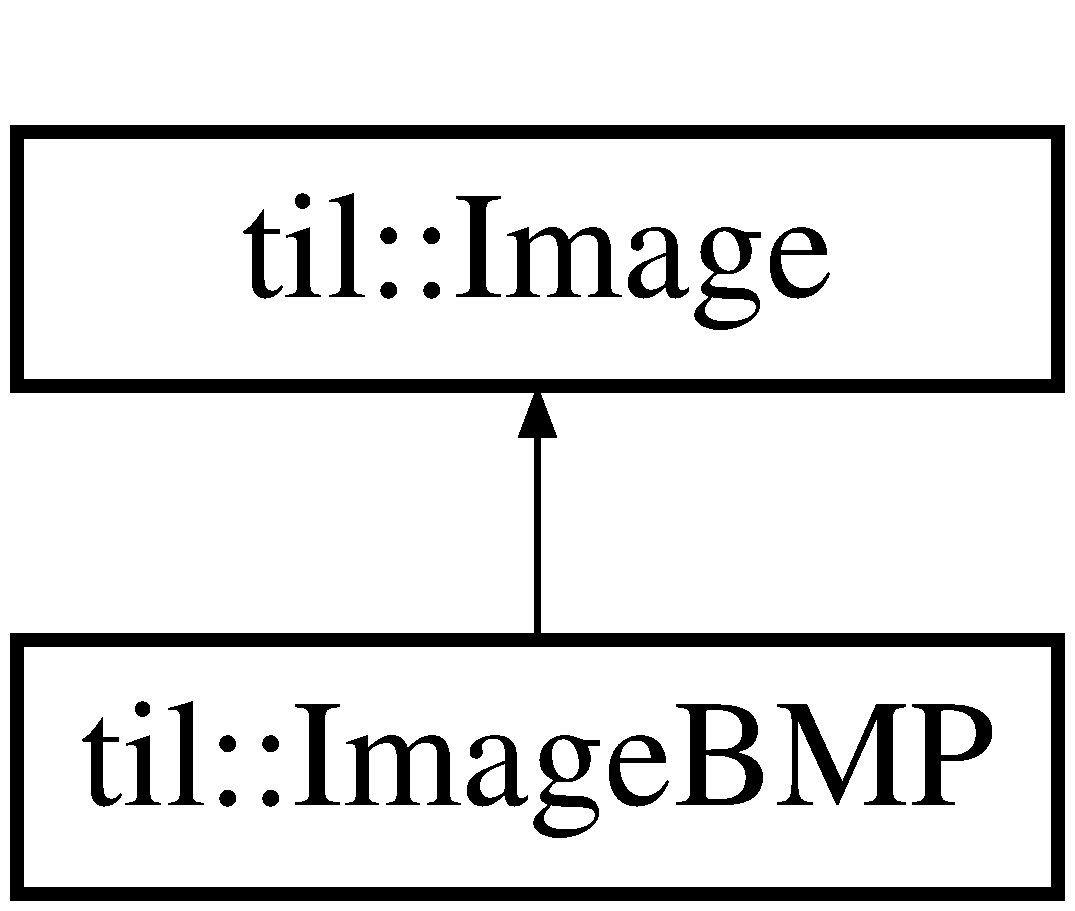
\includegraphics[height=2.000000cm]{classtil_1_1_image_b_m_p}
\end{center}
\end{figure}
\subsection*{Public Member Functions}
\begin{DoxyCompactItemize}
\item 
bool \hyperlink{classtil_1_1_image_b_m_p_a268aad59d643b44370d934c756735ad0}{Parse} (\hyperlink{namespacetil_a20db61688ed403d11f057a508d87e54c}{uint32} a\_\-ColorDepth)
\begin{DoxyCompactList}\small\item\em Parses the actual image data. \item\end{DoxyCompactList}\item 
\hyperlink{namespacetil_a20db61688ed403d11f057a508d87e54c}{uint32} \hyperlink{classtil_1_1_image_b_m_p_a8a3a00823903dfd0e3b83b5b499d88f7}{GetFrameCount} ()
\begin{DoxyCompactList}\small\item\em Returns the amount of frames this image contains. \item\end{DoxyCompactList}\item 
\hyperlink{namespacetil_a5f3ec10aca1a788b495a0bd3787bc2dc}{byte} $\ast$ \hyperlink{classtil_1_1_image_b_m_p_a2a667c1f36e310f0040bfabc36fad6ba}{GetPixels} (\hyperlink{namespacetil_a20db61688ed403d11f057a508d87e54c}{uint32} a\_\-Frame=0)
\begin{DoxyCompactList}\small\item\em Get the pixel data from this image. \item\end{DoxyCompactList}\item 
\hyperlink{namespacetil_a20db61688ed403d11f057a508d87e54c}{uint32} \hyperlink{classtil_1_1_image_b_m_p_a107a758c2401e017af7645a257b27581}{GetWidth} (\hyperlink{namespacetil_a20db61688ed403d11f057a508d87e54c}{uint32} a\_\-Frame=0)
\begin{DoxyCompactList}\small\item\em Get the width of a frame. \item\end{DoxyCompactList}\item 
\hyperlink{namespacetil_a20db61688ed403d11f057a508d87e54c}{uint32} \hyperlink{classtil_1_1_image_b_m_p_a9f6236bf4b43264f9b729a83a850a62b}{GetHeight} (\hyperlink{namespacetil_a20db61688ed403d11f057a508d87e54c}{uint32} a\_\-Frame=0)
\begin{DoxyCompactList}\small\item\em Get the height of a frame. \item\end{DoxyCompactList}\end{DoxyCompactItemize}


\subsection{Detailed Description}
\hyperlink{classtil_1_1_image}{til::Image} implementation of a BMP loader. 

\subsection{Member Function Documentation}
\hypertarget{classtil_1_1_image_b_m_p_a8a3a00823903dfd0e3b83b5b499d88f7}{
\index{til::ImageBMP@{til::ImageBMP}!GetFrameCount@{GetFrameCount}}
\index{GetFrameCount@{GetFrameCount}!til::ImageBMP@{til::ImageBMP}}
\subsubsection[{GetFrameCount}]{\setlength{\rightskip}{0pt plus 5cm}{\bf uint32} til::ImageBMP::GetFrameCount (
\begin{DoxyParamCaption}
{}
\end{DoxyParamCaption}
)\hspace{0.3cm}{\ttfamily  \mbox{[}virtual\mbox{]}}}}
\label{classtil_1_1_image_b_m_p_a8a3a00823903dfd0e3b83b5b499d88f7}


Returns the amount of frames this image contains. 

Used when dealing with formats that support animation or multiple images.

\begin{DoxyNote}{Note}
There is never going to be support for other video formats. This is because TinyImageLoader is an $\ast$image$\ast$ loader, not a video loader. The exception to the rule are GIF89 and APNG, because it concerns an extension to a normally single-\/framed format. 
\end{DoxyNote}


Reimplemented from \hyperlink{classtil_1_1_image_a78c10e07b535c99840b0afd5aa165df4}{til::Image}.

\hypertarget{classtil_1_1_image_b_m_p_a9f6236bf4b43264f9b729a83a850a62b}{
\index{til::ImageBMP@{til::ImageBMP}!GetHeight@{GetHeight}}
\index{GetHeight@{GetHeight}!til::ImageBMP@{til::ImageBMP}}
\subsubsection[{GetHeight}]{\setlength{\rightskip}{0pt plus 5cm}{\bf uint32} til::ImageBMP::GetHeight (
\begin{DoxyParamCaption}
\item[{{\bf uint32}}]{a\_\-Frame = {\ttfamily 0}}
\end{DoxyParamCaption}
)\hspace{0.3cm}{\ttfamily  \mbox{[}virtual\mbox{]}}}}
\label{classtil_1_1_image_b_m_p_a9f6236bf4b43264f9b729a83a850a62b}


Get the height of a frame. 


\begin{DoxyParams}{Parameters}
{\em a\_\-Frame} & The frame of an animation or image to return.\\
\hline
\end{DoxyParams}
\begin{DoxyReturn}{Returns}
The height as a uint32.
\end{DoxyReturn}
Some formats support multiple frames or images with different dimensions. You can call this function with a frame number to get the correct dimensions. 

Implements \hyperlink{classtil_1_1_image_ad623add911ba5230f56a4cc58af75ec1}{til::Image}.

\hypertarget{classtil_1_1_image_b_m_p_a2a667c1f36e310f0040bfabc36fad6ba}{
\index{til::ImageBMP@{til::ImageBMP}!GetPixels@{GetPixels}}
\index{GetPixels@{GetPixels}!til::ImageBMP@{til::ImageBMP}}
\subsubsection[{GetPixels}]{\setlength{\rightskip}{0pt plus 5cm}{\bf byte}$\ast$ til::ImageBMP::GetPixels (
\begin{DoxyParamCaption}
\item[{{\bf uint32}}]{a\_\-Frame = {\ttfamily 0}}
\end{DoxyParamCaption}
)\hspace{0.3cm}{\ttfamily  \mbox{[}virtual\mbox{]}}}}
\label{classtil_1_1_image_b_m_p_a2a667c1f36e310f0040bfabc36fad6ba}


Get the pixel data from this image. 


\begin{DoxyParams}{Parameters}
{\em a\_\-Frame} & The frame of an animation to return.\\
\hline
\end{DoxyParams}
\begin{DoxyReturn}{Returns}
Pixel array as a byte array.
\end{DoxyReturn}
The data is encoded according to the color depth specified. For instance, when loading images as 32-\/bit ARGB, the stream of bytes must be converted to unsigned long before being used.


\begin{DoxyCode}
                        til::Image* load = TIL_Load("media\\texture.png", 
      TIL_DEPTH_A8B8G8R8 | TIL_FILE_ADDWORKINGDIR);
                        unsigned long* pixels = (unsigned long*)load->GetPixels()
      ;
\end{DoxyCode}
 

Implements \hyperlink{classtil_1_1_image_a8dd46f6477025e23dc921e1a4a3f6a62}{til::Image}.

\hypertarget{classtil_1_1_image_b_m_p_a107a758c2401e017af7645a257b27581}{
\index{til::ImageBMP@{til::ImageBMP}!GetWidth@{GetWidth}}
\index{GetWidth@{GetWidth}!til::ImageBMP@{til::ImageBMP}}
\subsubsection[{GetWidth}]{\setlength{\rightskip}{0pt plus 5cm}{\bf uint32} til::ImageBMP::GetWidth (
\begin{DoxyParamCaption}
\item[{{\bf uint32}}]{a\_\-Frame = {\ttfamily 0}}
\end{DoxyParamCaption}
)\hspace{0.3cm}{\ttfamily  \mbox{[}virtual\mbox{]}}}}
\label{classtil_1_1_image_b_m_p_a107a758c2401e017af7645a257b27581}


Get the width of a frame. 


\begin{DoxyParams}{Parameters}
{\em a\_\-Frame} & The frame of an animation or image to return.\\
\hline
\end{DoxyParams}
\begin{DoxyReturn}{Returns}
The width as a uint32.
\end{DoxyReturn}
Some formats support multiple frames or images with different dimensions. You can call this function with a frame number to get the correct dimensions. 

Implements \hyperlink{classtil_1_1_image_a769be7e5a2cc490e8ae70b7c29a56eca}{til::Image}.

\hypertarget{classtil_1_1_image_b_m_p_a268aad59d643b44370d934c756735ad0}{
\index{til::ImageBMP@{til::ImageBMP}!Parse@{Parse}}
\index{Parse@{Parse}!til::ImageBMP@{til::ImageBMP}}
\subsubsection[{Parse}]{\setlength{\rightskip}{0pt plus 5cm}bool til::ImageBMP::Parse (
\begin{DoxyParamCaption}
\item[{{\bf uint32}}]{a\_\-ColorDepth}
\end{DoxyParamCaption}
)\hspace{0.3cm}{\ttfamily  \mbox{[}virtual\mbox{]}}}}
\label{classtil_1_1_image_b_m_p_a268aad59d643b44370d934c756735ad0}


Parses the actual image data. 


\begin{DoxyParams}{Parameters}
{\em a\_\-ColorDepth} & The color depth received from \hyperlink{classtil_1_1_image_ae1202f84c0addb81eba161f746a9d4cc}{SetBPP};\\
\hline
\end{DoxyParams}
This method is pure virtual and should be overwritten by an image loading implementation. 

Implements \hyperlink{classtil_1_1_image_a2436c982f6b403ab07591f06107fe432}{til::Image}.



The documentation for this class was generated from the following file:\begin{DoxyCompactItemize}
\item 
SDK/headers/\hyperlink{_t_i_l_image_b_m_p_8h}{TILImageBMP.h}\end{DoxyCompactItemize}

\hypertarget{classtil_1_1_image_d_d_s}{
\section{til::ImageDDS Class Reference}
\label{classtil_1_1_image_d_d_s}\index{til::ImageDDS@{til::ImageDDS}}
}


Implementation of a DDS loader.  




{\ttfamily \#include $<$TILImageDDS.h$>$}

Inheritance diagram for til::ImageDDS:\begin{figure}[H]
\begin{center}
\leavevmode
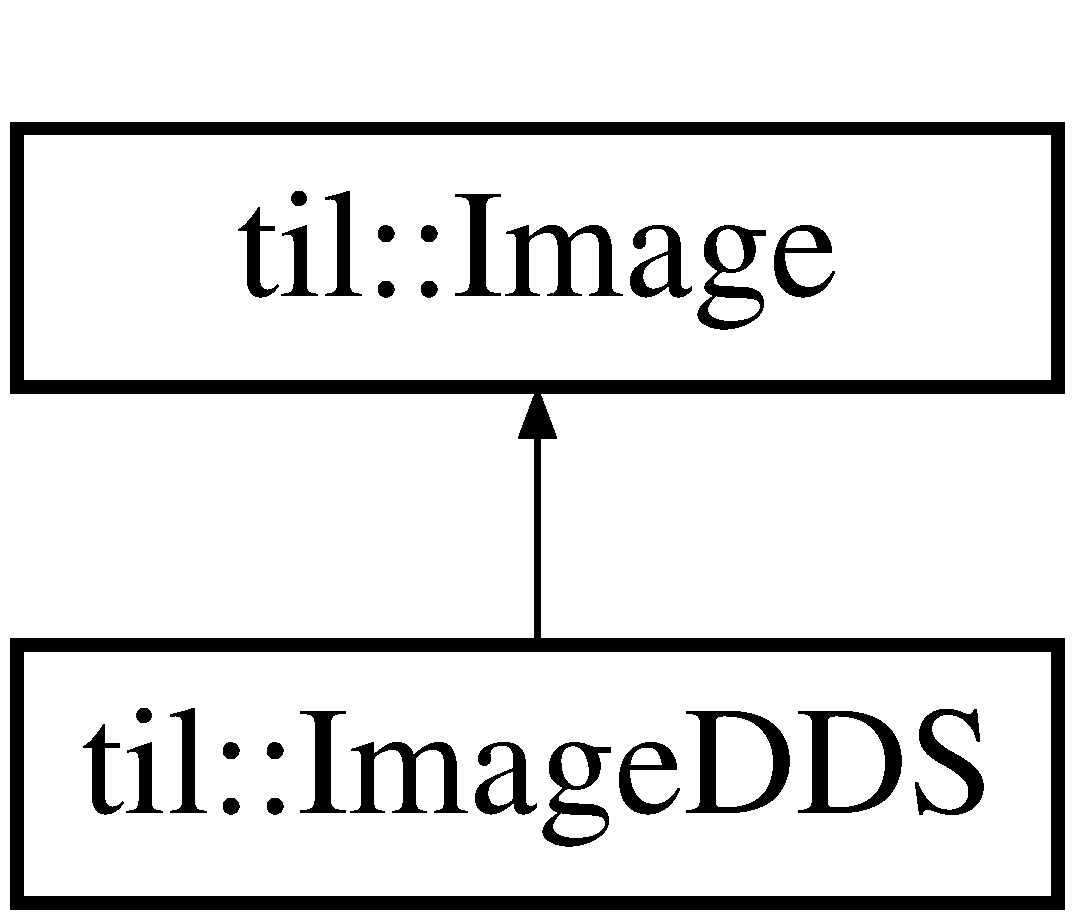
\includegraphics[height=2.000000cm]{classtil_1_1_image_d_d_s}
\end{center}
\end{figure}
\subsection*{Public Member Functions}
\begin{DoxyCompactItemize}
\item 
\hyperlink{namespacetil_a20db61688ed403d11f057a508d87e54c}{uint32} \hyperlink{classtil_1_1_image_d_d_s_a616b077809ea2a4ebde9fa53651c198a}{GetFrameCount} ()
\begin{DoxyCompactList}\small\item\em Returns the amount of frames this image contains. \item\end{DoxyCompactList}\item 
\hyperlink{namespacetil_a5f3ec10aca1a788b495a0bd3787bc2dc}{byte} $\ast$ \hyperlink{classtil_1_1_image_d_d_s_ac14aad199b3430d527610f38498faa9e}{GetPixels} (\hyperlink{namespacetil_a20db61688ed403d11f057a508d87e54c}{uint32} a\_\-Frame=0)
\begin{DoxyCompactList}\small\item\em Get the pixel data from this image. \item\end{DoxyCompactList}\item 
\hyperlink{namespacetil_a20db61688ed403d11f057a508d87e54c}{uint32} \hyperlink{classtil_1_1_image_d_d_s_adde03a6b7297091d566c20ae2e24d35d}{GetWidth} (\hyperlink{namespacetil_a20db61688ed403d11f057a508d87e54c}{uint32} a\_\-Frame=0)
\begin{DoxyCompactList}\small\item\em Get the width of a frame. \item\end{DoxyCompactList}\item 
\hyperlink{namespacetil_a20db61688ed403d11f057a508d87e54c}{uint32} \hyperlink{classtil_1_1_image_d_d_s_a9ae6dc6b71a3a056eecd8b756d9089e8}{GetHeight} (\hyperlink{namespacetil_a20db61688ed403d11f057a508d87e54c}{uint32} a\_\-Frame=0)
\begin{DoxyCompactList}\small\item\em Get the height of a frame. \item\end{DoxyCompactList}\item 
bool \hyperlink{classtil_1_1_image_d_d_s_a65def4c46d0da0c6600310c3dcb86cef}{Parse} (\hyperlink{namespacetil_a20db61688ed403d11f057a508d87e54c}{uint32} a\_\-ColorDepth)
\begin{DoxyCompactList}\small\item\em Parses the actual image data. \item\end{DoxyCompactList}\end{DoxyCompactItemize}


\subsection{Detailed Description}
Implementation of a DDS loader. 

\subsection{Member Function Documentation}
\hypertarget{classtil_1_1_image_d_d_s_a616b077809ea2a4ebde9fa53651c198a}{
\index{til::ImageDDS@{til::ImageDDS}!GetFrameCount@{GetFrameCount}}
\index{GetFrameCount@{GetFrameCount}!til::ImageDDS@{til::ImageDDS}}
\subsubsection[{GetFrameCount}]{\setlength{\rightskip}{0pt plus 5cm}{\bf uint32} til::ImageDDS::GetFrameCount (
\begin{DoxyParamCaption}
{}
\end{DoxyParamCaption}
)\hspace{0.3cm}{\ttfamily  \mbox{[}virtual\mbox{]}}}}
\label{classtil_1_1_image_d_d_s_a616b077809ea2a4ebde9fa53651c198a}


Returns the amount of frames this image contains. 

Used when dealing with formats that support animation or multiple images.

\begin{DoxyNote}{Note}
There is never going to be support for other video formats. This is because TinyImageLoader is an $\ast$image$\ast$ loader, not a video loader. The exception to the rule are GIF89 and APNG, because it concerns an extension to a normally single-\/framed format. 
\end{DoxyNote}


Reimplemented from \hyperlink{classtil_1_1_image_a78c10e07b535c99840b0afd5aa165df4}{til::Image}.

\hypertarget{classtil_1_1_image_d_d_s_a9ae6dc6b71a3a056eecd8b756d9089e8}{
\index{til::ImageDDS@{til::ImageDDS}!GetHeight@{GetHeight}}
\index{GetHeight@{GetHeight}!til::ImageDDS@{til::ImageDDS}}
\subsubsection[{GetHeight}]{\setlength{\rightskip}{0pt plus 5cm}{\bf uint32} til::ImageDDS::GetHeight (
\begin{DoxyParamCaption}
\item[{{\bf uint32}}]{a\_\-Frame = {\ttfamily 0}}
\end{DoxyParamCaption}
)\hspace{0.3cm}{\ttfamily  \mbox{[}virtual\mbox{]}}}}
\label{classtil_1_1_image_d_d_s_a9ae6dc6b71a3a056eecd8b756d9089e8}


Get the height of a frame. 


\begin{DoxyParams}{Parameters}
{\em a\_\-Frame} & The frame of an animation or image to return.\\
\hline
\end{DoxyParams}
\begin{DoxyReturn}{Returns}
The height as a uint32.
\end{DoxyReturn}
Some formats support multiple frames or images with different dimensions. You can call this function with a frame number to get the correct dimensions. 

Implements \hyperlink{classtil_1_1_image_ad623add911ba5230f56a4cc58af75ec1}{til::Image}.

\hypertarget{classtil_1_1_image_d_d_s_ac14aad199b3430d527610f38498faa9e}{
\index{til::ImageDDS@{til::ImageDDS}!GetPixels@{GetPixels}}
\index{GetPixels@{GetPixels}!til::ImageDDS@{til::ImageDDS}}
\subsubsection[{GetPixels}]{\setlength{\rightskip}{0pt plus 5cm}{\bf byte}$\ast$ til::ImageDDS::GetPixels (
\begin{DoxyParamCaption}
\item[{{\bf uint32}}]{a\_\-Frame = {\ttfamily 0}}
\end{DoxyParamCaption}
)\hspace{0.3cm}{\ttfamily  \mbox{[}virtual\mbox{]}}}}
\label{classtil_1_1_image_d_d_s_ac14aad199b3430d527610f38498faa9e}


Get the pixel data from this image. 


\begin{DoxyParams}{Parameters}
{\em a\_\-Frame} & The frame of an animation to return.\\
\hline
\end{DoxyParams}
\begin{DoxyReturn}{Returns}
Pixel array as a byte array.
\end{DoxyReturn}
The data is encoded according to the color depth specified. For instance, when loading images as 32-\/bit ARGB, the stream of bytes must be converted to unsigned long before being used.


\begin{DoxyCode}
                        til::Image* load = TIL_Load("media\\texture.png", 
      TIL_DEPTH_A8B8G8R8 | TIL_FILE_ADDWORKINGDIR);
                        unsigned long* pixels = (unsigned long*)load->GetPixels()
      ;
\end{DoxyCode}
 

Implements \hyperlink{classtil_1_1_image_a8dd46f6477025e23dc921e1a4a3f6a62}{til::Image}.

\hypertarget{classtil_1_1_image_d_d_s_adde03a6b7297091d566c20ae2e24d35d}{
\index{til::ImageDDS@{til::ImageDDS}!GetWidth@{GetWidth}}
\index{GetWidth@{GetWidth}!til::ImageDDS@{til::ImageDDS}}
\subsubsection[{GetWidth}]{\setlength{\rightskip}{0pt plus 5cm}{\bf uint32} til::ImageDDS::GetWidth (
\begin{DoxyParamCaption}
\item[{{\bf uint32}}]{a\_\-Frame = {\ttfamily 0}}
\end{DoxyParamCaption}
)\hspace{0.3cm}{\ttfamily  \mbox{[}virtual\mbox{]}}}}
\label{classtil_1_1_image_d_d_s_adde03a6b7297091d566c20ae2e24d35d}


Get the width of a frame. 


\begin{DoxyParams}{Parameters}
{\em a\_\-Frame} & The frame of an animation or image to return.\\
\hline
\end{DoxyParams}
\begin{DoxyReturn}{Returns}
The width as a uint32.
\end{DoxyReturn}
Some formats support multiple frames or images with different dimensions. You can call this function with a frame number to get the correct dimensions. 

Implements \hyperlink{classtil_1_1_image_a769be7e5a2cc490e8ae70b7c29a56eca}{til::Image}.

\hypertarget{classtil_1_1_image_d_d_s_a65def4c46d0da0c6600310c3dcb86cef}{
\index{til::ImageDDS@{til::ImageDDS}!Parse@{Parse}}
\index{Parse@{Parse}!til::ImageDDS@{til::ImageDDS}}
\subsubsection[{Parse}]{\setlength{\rightskip}{0pt plus 5cm}bool til::ImageDDS::Parse (
\begin{DoxyParamCaption}
\item[{{\bf uint32}}]{a\_\-ColorDepth}
\end{DoxyParamCaption}
)\hspace{0.3cm}{\ttfamily  \mbox{[}virtual\mbox{]}}}}
\label{classtil_1_1_image_d_d_s_a65def4c46d0da0c6600310c3dcb86cef}


Parses the actual image data. 


\begin{DoxyParams}{Parameters}
{\em a\_\-ColorDepth} & The color depth received from \hyperlink{classtil_1_1_image_ae1202f84c0addb81eba161f746a9d4cc}{SetBPP};\\
\hline
\end{DoxyParams}
This method is pure virtual and should be overwritten by an image loading implementation. 

Implements \hyperlink{classtil_1_1_image_a2436c982f6b403ab07591f06107fe432}{til::Image}.



The documentation for this class was generated from the following file:\begin{DoxyCompactItemize}
\item 
SDK/headers/\hyperlink{_t_i_l_image_d_d_s_8h}{TILImageDDS.h}\end{DoxyCompactItemize}

\hypertarget{classtil_1_1_image_g_i_f}{
\section{til::ImageGIF Class Reference}
\label{classtil_1_1_image_g_i_f}\index{til::ImageGIF@{til::ImageGIF}}
}


\hyperlink{classtil_1_1_image}{til::Image} implementation of a GIF loader.  




{\ttfamily \#include $<$TILImageGIF.h$>$}

Inheritance diagram for til::ImageGIF:\begin{figure}[H]
\begin{center}
\leavevmode
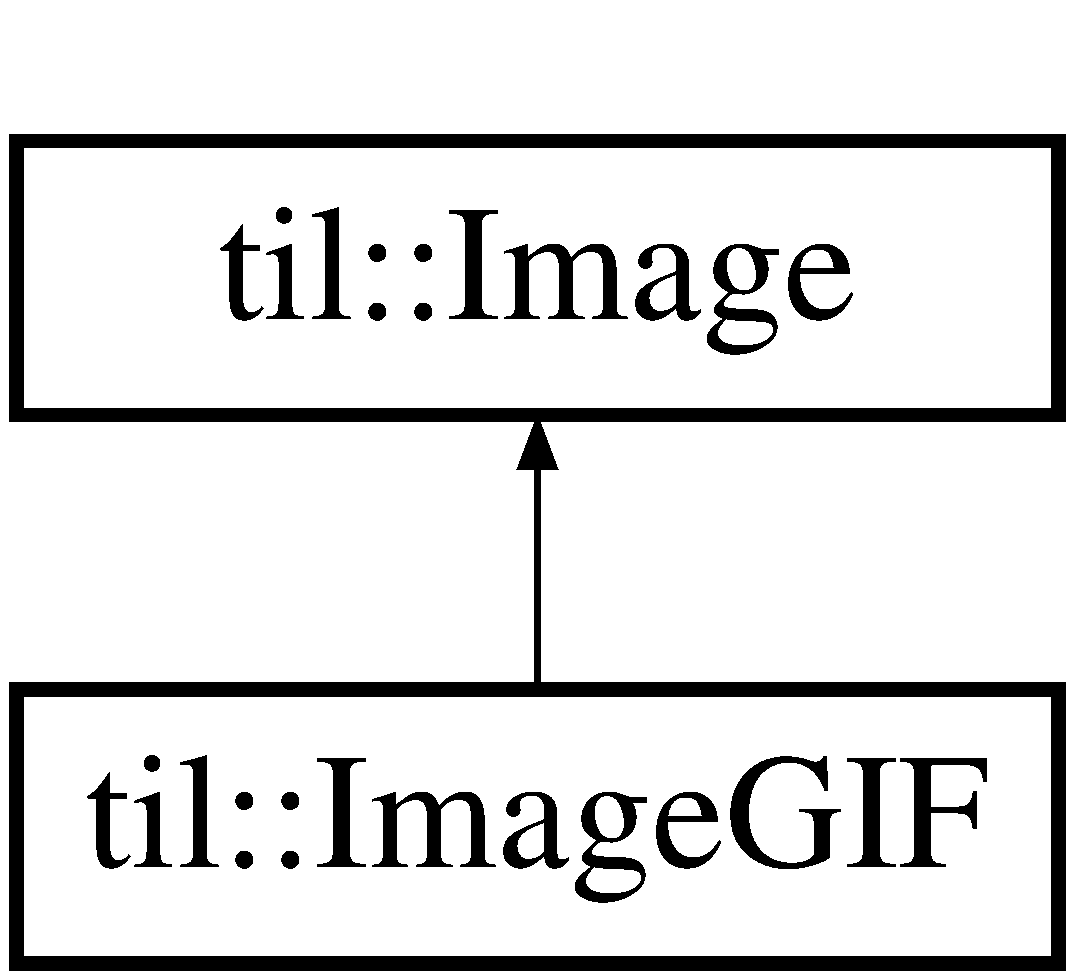
\includegraphics[height=2.000000cm]{classtil_1_1_image_g_i_f}
\end{center}
\end{figure}
\subsection*{Public Member Functions}
\begin{DoxyCompactItemize}
\item 
bool \hyperlink{classtil_1_1_image_g_i_f_a227eb60dcc93f3a9390ef3b5152d8dd4}{Parse} (\hyperlink{namespacetil_a20db61688ed403d11f057a508d87e54c}{uint32} a\_\-ColorDepth)
\begin{DoxyCompactList}\small\item\em Parses the actual image data. \item\end{DoxyCompactList}\item 
\hyperlink{namespacetil_a20db61688ed403d11f057a508d87e54c}{uint32} \hyperlink{classtil_1_1_image_g_i_f_a9e0c056b0263196d305c9102f254240e}{GetFrameCount} ()
\begin{DoxyCompactList}\small\item\em Returns the amount of frames this image contains. \item\end{DoxyCompactList}\item 
float \hyperlink{classtil_1_1_image_g_i_f_a01af14634200dbb109d124746764d05d}{GetDelay} ()
\begin{DoxyCompactList}\small\item\em Returns the delay between frames. \item\end{DoxyCompactList}\item 
\hyperlink{namespacetil_a5f3ec10aca1a788b495a0bd3787bc2dc}{byte} $\ast$ \hyperlink{classtil_1_1_image_g_i_f_ad9ee66121f0d4fe3a58af75177bb9245}{GetPixels} (\hyperlink{namespacetil_a20db61688ed403d11f057a508d87e54c}{uint32} a\_\-Frame=0)
\begin{DoxyCompactList}\small\item\em Get the pixel data from this image. \item\end{DoxyCompactList}\item 
\hyperlink{namespacetil_a20db61688ed403d11f057a508d87e54c}{uint32} \hyperlink{classtil_1_1_image_g_i_f_a368dce7e854e1eddad76242aac167161}{GetWidth} (\hyperlink{namespacetil_a20db61688ed403d11f057a508d87e54c}{uint32} a\_\-Frame=0)
\begin{DoxyCompactList}\small\item\em Get the width of a frame. \item\end{DoxyCompactList}\item 
\hyperlink{namespacetil_a20db61688ed403d11f057a508d87e54c}{uint32} \hyperlink{classtil_1_1_image_g_i_f_ac241e6cacaf14d1e73aae50f105450ae}{GetHeight} (\hyperlink{namespacetil_a20db61688ed403d11f057a508d87e54c}{uint32} a\_\-Frame=0)
\begin{DoxyCompactList}\small\item\em Get the height of a frame. \item\end{DoxyCompactList}\end{DoxyCompactItemize}
\begin{Indent}{\bf Internal}\par
{\em These functions are internal and shouldn't be called by developers. }\begin{DoxyCompactItemize}
\item 
\hypertarget{classtil_1_1_image_g_i_f_a2f6cb7c81ae1e447af51b6683597cbf0}{
void {\bfseries AddBuffer} ()}
\label{classtil_1_1_image_g_i_f_a2f6cb7c81ae1e447af51b6683597cbf0}

\item 
\hypertarget{classtil_1_1_image_g_i_f_adaaf9bb4a81c18708e29b08bfbd25faf}{
void {\bfseries CompileColors} (bool a\_\-LocalTable=true)}
\label{classtil_1_1_image_g_i_f_adaaf9bb4a81c18708e29b08bfbd25faf}

\item 
\hypertarget{classtil_1_1_image_g_i_f_ad0e4c41f345cad3e2dae37eb7874b6a0}{
void {\bfseries ReleaseMemory} (BufferLinked $\ast$a\_\-Buffer)}
\label{classtil_1_1_image_g_i_f_ad0e4c41f345cad3e2dae37eb7874b6a0}

\end{DoxyCompactItemize}
\end{Indent}


\subsection{Detailed Description}
\hyperlink{classtil_1_1_image}{til::Image} implementation of a GIF loader. 

\subsection{Member Function Documentation}
\hypertarget{classtil_1_1_image_g_i_f_a01af14634200dbb109d124746764d05d}{
\index{til::ImageGIF@{til::ImageGIF}!GetDelay@{GetDelay}}
\index{GetDelay@{GetDelay}!til::ImageGIF@{til::ImageGIF}}
\subsubsection[{GetDelay}]{\setlength{\rightskip}{0pt plus 5cm}float til::ImageGIF::GetDelay (
\begin{DoxyParamCaption}
{}
\end{DoxyParamCaption}
)\hspace{0.3cm}{\ttfamily  \mbox{[}virtual\mbox{]}}}}
\label{classtil_1_1_image_g_i_f_a01af14634200dbb109d124746764d05d}


Returns the delay between frames. 

\begin{DoxyReturn}{Returns}
The delay in seconds between frames
\end{DoxyReturn}
Used when dealing with formats that support animation. 

Reimplemented from \hyperlink{classtil_1_1_image_aabddc7f03e3d1962f5abb21c200f2050}{til::Image}.

\hypertarget{classtil_1_1_image_g_i_f_a9e0c056b0263196d305c9102f254240e}{
\index{til::ImageGIF@{til::ImageGIF}!GetFrameCount@{GetFrameCount}}
\index{GetFrameCount@{GetFrameCount}!til::ImageGIF@{til::ImageGIF}}
\subsubsection[{GetFrameCount}]{\setlength{\rightskip}{0pt plus 5cm}{\bf uint32} til::ImageGIF::GetFrameCount (
\begin{DoxyParamCaption}
{}
\end{DoxyParamCaption}
)\hspace{0.3cm}{\ttfamily  \mbox{[}virtual\mbox{]}}}}
\label{classtil_1_1_image_g_i_f_a9e0c056b0263196d305c9102f254240e}


Returns the amount of frames this image contains. 

Used when dealing with formats that support animation or multiple images.

\begin{DoxyNote}{Note}
There is never going to be support for other video formats. This is because TinyImageLoader is an $\ast$image$\ast$ loader, not a video loader. The exception to the rule are GIF89 and APNG, because it concerns an extension to a normally single-\/framed format. 
\end{DoxyNote}


Reimplemented from \hyperlink{classtil_1_1_image_a78c10e07b535c99840b0afd5aa165df4}{til::Image}.

\hypertarget{classtil_1_1_image_g_i_f_ac241e6cacaf14d1e73aae50f105450ae}{
\index{til::ImageGIF@{til::ImageGIF}!GetHeight@{GetHeight}}
\index{GetHeight@{GetHeight}!til::ImageGIF@{til::ImageGIF}}
\subsubsection[{GetHeight}]{\setlength{\rightskip}{0pt plus 5cm}{\bf uint32} til::ImageGIF::GetHeight (
\begin{DoxyParamCaption}
\item[{{\bf uint32}}]{a\_\-Frame = {\ttfamily 0}}
\end{DoxyParamCaption}
)\hspace{0.3cm}{\ttfamily  \mbox{[}virtual\mbox{]}}}}
\label{classtil_1_1_image_g_i_f_ac241e6cacaf14d1e73aae50f105450ae}


Get the height of a frame. 


\begin{DoxyParams}{Parameters}
{\em a\_\-Frame} & The frame of an animation or image to return.\\
\hline
\end{DoxyParams}
\begin{DoxyReturn}{Returns}
The height as a uint32.
\end{DoxyReturn}
Some formats support multiple frames or images with different dimensions. You can call this function with a frame number to get the correct dimensions. 

Implements \hyperlink{classtil_1_1_image_ad623add911ba5230f56a4cc58af75ec1}{til::Image}.

\hypertarget{classtil_1_1_image_g_i_f_ad9ee66121f0d4fe3a58af75177bb9245}{
\index{til::ImageGIF@{til::ImageGIF}!GetPixels@{GetPixels}}
\index{GetPixels@{GetPixels}!til::ImageGIF@{til::ImageGIF}}
\subsubsection[{GetPixels}]{\setlength{\rightskip}{0pt plus 5cm}{\bf byte}$\ast$ til::ImageGIF::GetPixels (
\begin{DoxyParamCaption}
\item[{{\bf uint32}}]{a\_\-Frame = {\ttfamily 0}}
\end{DoxyParamCaption}
)\hspace{0.3cm}{\ttfamily  \mbox{[}virtual\mbox{]}}}}
\label{classtil_1_1_image_g_i_f_ad9ee66121f0d4fe3a58af75177bb9245}


Get the pixel data from this image. 


\begin{DoxyParams}{Parameters}
{\em a\_\-Frame} & The frame of an animation to return.\\
\hline
\end{DoxyParams}
\begin{DoxyReturn}{Returns}
Pixel array as a byte array.
\end{DoxyReturn}
The data is encoded according to the color depth specified. For instance, when loading images as 32-\/bit ARGB, the stream of bytes must be converted to unsigned long before being used.


\begin{DoxyCode}
                        til::Image* load = TIL_Load("media\\texture.png", 
      TIL_DEPTH_A8B8G8R8 | TIL_FILE_ADDWORKINGDIR);
                        unsigned long* pixels = (unsigned long*)load->GetPixels()
      ;
\end{DoxyCode}
 

Implements \hyperlink{classtil_1_1_image_a8dd46f6477025e23dc921e1a4a3f6a62}{til::Image}.

\hypertarget{classtil_1_1_image_g_i_f_a368dce7e854e1eddad76242aac167161}{
\index{til::ImageGIF@{til::ImageGIF}!GetWidth@{GetWidth}}
\index{GetWidth@{GetWidth}!til::ImageGIF@{til::ImageGIF}}
\subsubsection[{GetWidth}]{\setlength{\rightskip}{0pt plus 5cm}{\bf uint32} til::ImageGIF::GetWidth (
\begin{DoxyParamCaption}
\item[{{\bf uint32}}]{a\_\-Frame = {\ttfamily 0}}
\end{DoxyParamCaption}
)\hspace{0.3cm}{\ttfamily  \mbox{[}virtual\mbox{]}}}}
\label{classtil_1_1_image_g_i_f_a368dce7e854e1eddad76242aac167161}


Get the width of a frame. 


\begin{DoxyParams}{Parameters}
{\em a\_\-Frame} & The frame of an animation or image to return.\\
\hline
\end{DoxyParams}
\begin{DoxyReturn}{Returns}
The width as a uint32.
\end{DoxyReturn}
Some formats support multiple frames or images with different dimensions. You can call this function with a frame number to get the correct dimensions. 

Implements \hyperlink{classtil_1_1_image_a769be7e5a2cc490e8ae70b7c29a56eca}{til::Image}.

\hypertarget{classtil_1_1_image_g_i_f_a227eb60dcc93f3a9390ef3b5152d8dd4}{
\index{til::ImageGIF@{til::ImageGIF}!Parse@{Parse}}
\index{Parse@{Parse}!til::ImageGIF@{til::ImageGIF}}
\subsubsection[{Parse}]{\setlength{\rightskip}{0pt plus 5cm}bool til::ImageGIF::Parse (
\begin{DoxyParamCaption}
\item[{{\bf uint32}}]{a\_\-ColorDepth}
\end{DoxyParamCaption}
)\hspace{0.3cm}{\ttfamily  \mbox{[}virtual\mbox{]}}}}
\label{classtil_1_1_image_g_i_f_a227eb60dcc93f3a9390ef3b5152d8dd4}


Parses the actual image data. 


\begin{DoxyParams}{Parameters}
{\em a\_\-ColorDepth} & The color depth received from \hyperlink{classtil_1_1_image_ae1202f84c0addb81eba161f746a9d4cc}{SetBPP};\\
\hline
\end{DoxyParams}
This method is pure virtual and should be overwritten by an image loading implementation. 

Implements \hyperlink{classtil_1_1_image_a2436c982f6b403ab07591f06107fe432}{til::Image}.



The documentation for this class was generated from the following file:\begin{DoxyCompactItemize}
\item 
SDK/headers/\hyperlink{_t_i_l_image_g_i_f_8h}{TILImageGIF.h}\end{DoxyCompactItemize}

\hypertarget{classtil_1_1_image_i_c_o}{
\section{til::ImageICO Class Reference}
\label{classtil_1_1_image_i_c_o}\index{til::ImageICO@{til::ImageICO}}
}


\hyperlink{classtil_1_1_image}{til::Image} implementation of an ICO loader.  




{\ttfamily \#include $<$TILImageICO.h$>$}

Inheritance diagram for til::ImageICO:\begin{figure}[H]
\begin{center}
\leavevmode
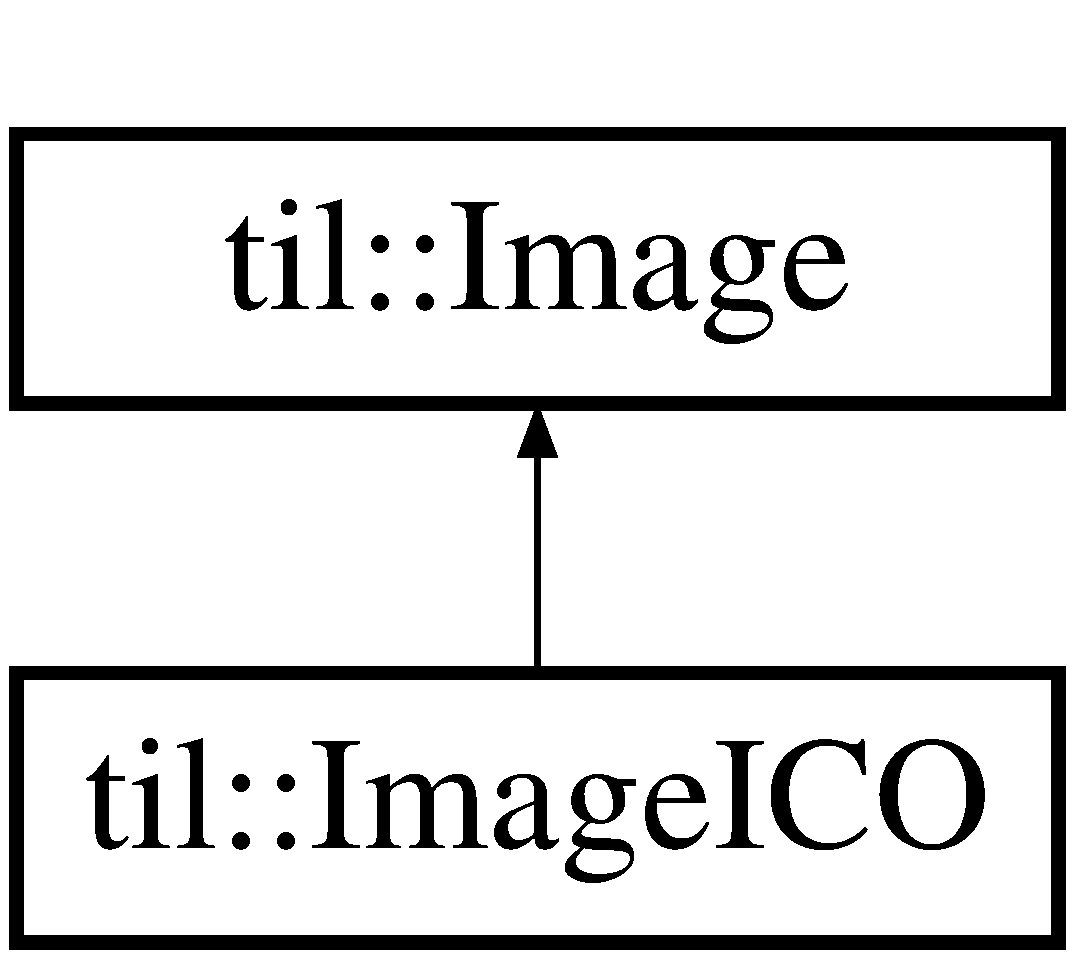
\includegraphics[height=2.000000cm]{classtil_1_1_image_i_c_o}
\end{center}
\end{figure}
\subsection*{Public Member Functions}
\begin{DoxyCompactItemize}
\item 
bool \hyperlink{classtil_1_1_image_i_c_o_a22b53abab2e8b944ae0b50d6246b5f96}{Parse} (\hyperlink{namespacetil_a20db61688ed403d11f057a508d87e54c}{uint32} a\_\-ColorDepth)
\begin{DoxyCompactList}\small\item\em Parses the actual image data. \item\end{DoxyCompactList}\item 
\hyperlink{namespacetil_a20db61688ed403d11f057a508d87e54c}{uint32} \hyperlink{classtil_1_1_image_i_c_o_a58280b473d5ebc9864ade082f2f0f96d}{GetFrameCount} ()
\begin{DoxyCompactList}\small\item\em Returns the amount of frames this image contains. \item\end{DoxyCompactList}\item 
\hyperlink{namespacetil_a5f3ec10aca1a788b495a0bd3787bc2dc}{byte} $\ast$ \hyperlink{classtil_1_1_image_i_c_o_a3501ed7aec07ea553855aff7cb58d7e8}{GetPixels} (\hyperlink{namespacetil_a20db61688ed403d11f057a508d87e54c}{uint32} a\_\-Frame=0)
\begin{DoxyCompactList}\small\item\em Get the pixel data from this image. \item\end{DoxyCompactList}\item 
\hyperlink{namespacetil_a20db61688ed403d11f057a508d87e54c}{uint32} \hyperlink{classtil_1_1_image_i_c_o_a0006ed86536bf2b91b8243bc3e95c282}{GetWidth} (\hyperlink{namespacetil_a20db61688ed403d11f057a508d87e54c}{uint32} a\_\-Frame=0)
\begin{DoxyCompactList}\small\item\em Get the width of a frame. \item\end{DoxyCompactList}\item 
\hyperlink{namespacetil_a20db61688ed403d11f057a508d87e54c}{uint32} \hyperlink{classtil_1_1_image_i_c_o_a9ae2f5e5d594f8b0a17690d72496605e}{GetHeight} (\hyperlink{namespacetil_a20db61688ed403d11f057a508d87e54c}{uint32} a\_\-Frame=0)
\begin{DoxyCompactList}\small\item\em Get the height of a frame. \item\end{DoxyCompactList}\end{DoxyCompactItemize}
\begin{Indent}{\bf Internal}\par
{\em These functions are internal and shouldn't be called by developers. }\begin{DoxyCompactItemize}
\item 
\hypertarget{classtil_1_1_image_i_c_o_a3f2b776b61aaa0e82962788f6b51ad8a}{
void {\bfseries AddBuffer} (\hyperlink{namespacetil_a20db61688ed403d11f057a508d87e54c}{uint32} a\_\-Width, \hyperlink{namespacetil_a20db61688ed403d11f057a508d87e54c}{uint32} a\_\-Height)}
\label{classtil_1_1_image_i_c_o_a3f2b776b61aaa0e82962788f6b51ad8a}

\item 
\hypertarget{classtil_1_1_image_i_c_o_a996ef9a436e8b0ac8af21e3af309bc2c}{
void {\bfseries ReleaseMemory} (BufferICO $\ast$a\_\-Buffer)}
\label{classtil_1_1_image_i_c_o_a996ef9a436e8b0ac8af21e3af309bc2c}

\item 
\hypertarget{classtil_1_1_image_i_c_o_ad0540439744a4e3c4a7debcab89b858c}{
void {\bfseries ExpandPalette} (BufferICO $\ast$a\_\-Buffer)}
\label{classtil_1_1_image_i_c_o_ad0540439744a4e3c4a7debcab89b858c}

\end{DoxyCompactItemize}
\end{Indent}


\subsection{Detailed Description}
\hyperlink{classtil_1_1_image}{til::Image} implementation of an ICO loader. 

\subsection{Member Function Documentation}
\hypertarget{classtil_1_1_image_i_c_o_a58280b473d5ebc9864ade082f2f0f96d}{
\index{til::ImageICO@{til::ImageICO}!GetFrameCount@{GetFrameCount}}
\index{GetFrameCount@{GetFrameCount}!til::ImageICO@{til::ImageICO}}
\subsubsection[{GetFrameCount}]{\setlength{\rightskip}{0pt plus 5cm}{\bf uint32} til::ImageICO::GetFrameCount (
\begin{DoxyParamCaption}
{}
\end{DoxyParamCaption}
)\hspace{0.3cm}{\ttfamily  \mbox{[}virtual\mbox{]}}}}
\label{classtil_1_1_image_i_c_o_a58280b473d5ebc9864ade082f2f0f96d}


Returns the amount of frames this image contains. 

Used when dealing with formats that support animation or multiple images.

\begin{DoxyNote}{Note}
There is never going to be support for other video formats. This is because TinyImageLoader is an $\ast$image$\ast$ loader, not a video loader. The exception to the rule are GIF89 and APNG, because it concerns an extension to a normally single-\/framed format. 
\end{DoxyNote}


Reimplemented from \hyperlink{classtil_1_1_image_a78c10e07b535c99840b0afd5aa165df4}{til::Image}.

\hypertarget{classtil_1_1_image_i_c_o_a9ae2f5e5d594f8b0a17690d72496605e}{
\index{til::ImageICO@{til::ImageICO}!GetHeight@{GetHeight}}
\index{GetHeight@{GetHeight}!til::ImageICO@{til::ImageICO}}
\subsubsection[{GetHeight}]{\setlength{\rightskip}{0pt plus 5cm}{\bf uint32} til::ImageICO::GetHeight (
\begin{DoxyParamCaption}
\item[{{\bf uint32}}]{a\_\-Frame = {\ttfamily 0}}
\end{DoxyParamCaption}
)\hspace{0.3cm}{\ttfamily  \mbox{[}virtual\mbox{]}}}}
\label{classtil_1_1_image_i_c_o_a9ae2f5e5d594f8b0a17690d72496605e}


Get the height of a frame. 


\begin{DoxyParams}{Parameters}
{\em a\_\-Frame} & The frame of an animation or image to return.\\
\hline
\end{DoxyParams}
\begin{DoxyReturn}{Returns}
The height as a uint32.
\end{DoxyReturn}
Some formats support multiple frames or images with different dimensions. You can call this function with a frame number to get the correct dimensions. 

Implements \hyperlink{classtil_1_1_image_ad623add911ba5230f56a4cc58af75ec1}{til::Image}.

\hypertarget{classtil_1_1_image_i_c_o_a3501ed7aec07ea553855aff7cb58d7e8}{
\index{til::ImageICO@{til::ImageICO}!GetPixels@{GetPixels}}
\index{GetPixels@{GetPixels}!til::ImageICO@{til::ImageICO}}
\subsubsection[{GetPixels}]{\setlength{\rightskip}{0pt plus 5cm}{\bf byte}$\ast$ til::ImageICO::GetPixels (
\begin{DoxyParamCaption}
\item[{{\bf uint32}}]{a\_\-Frame = {\ttfamily 0}}
\end{DoxyParamCaption}
)\hspace{0.3cm}{\ttfamily  \mbox{[}virtual\mbox{]}}}}
\label{classtil_1_1_image_i_c_o_a3501ed7aec07ea553855aff7cb58d7e8}


Get the pixel data from this image. 


\begin{DoxyParams}{Parameters}
{\em a\_\-Frame} & The frame of an animation to return.\\
\hline
\end{DoxyParams}
\begin{DoxyReturn}{Returns}
Pixel array as a byte array.
\end{DoxyReturn}
The data is encoded according to the color depth specified. For instance, when loading images as 32-\/bit ARGB, the stream of bytes must be converted to unsigned long before being used.


\begin{DoxyCode}
                        til::Image* load = TIL_Load("media\\texture.png", 
      TIL_DEPTH_A8B8G8R8 | TIL_FILE_ADDWORKINGDIR);
                        unsigned long* pixels = (unsigned long*)load->GetPixels()
      ;
\end{DoxyCode}
 

Implements \hyperlink{classtil_1_1_image_a8dd46f6477025e23dc921e1a4a3f6a62}{til::Image}.

\hypertarget{classtil_1_1_image_i_c_o_a0006ed86536bf2b91b8243bc3e95c282}{
\index{til::ImageICO@{til::ImageICO}!GetWidth@{GetWidth}}
\index{GetWidth@{GetWidth}!til::ImageICO@{til::ImageICO}}
\subsubsection[{GetWidth}]{\setlength{\rightskip}{0pt plus 5cm}{\bf uint32} til::ImageICO::GetWidth (
\begin{DoxyParamCaption}
\item[{{\bf uint32}}]{a\_\-Frame = {\ttfamily 0}}
\end{DoxyParamCaption}
)\hspace{0.3cm}{\ttfamily  \mbox{[}virtual\mbox{]}}}}
\label{classtil_1_1_image_i_c_o_a0006ed86536bf2b91b8243bc3e95c282}


Get the width of a frame. 


\begin{DoxyParams}{Parameters}
{\em a\_\-Frame} & The frame of an animation or image to return.\\
\hline
\end{DoxyParams}
\begin{DoxyReturn}{Returns}
The width as a uint32.
\end{DoxyReturn}
Some formats support multiple frames or images with different dimensions. You can call this function with a frame number to get the correct dimensions. 

Implements \hyperlink{classtil_1_1_image_a769be7e5a2cc490e8ae70b7c29a56eca}{til::Image}.

\hypertarget{classtil_1_1_image_i_c_o_a22b53abab2e8b944ae0b50d6246b5f96}{
\index{til::ImageICO@{til::ImageICO}!Parse@{Parse}}
\index{Parse@{Parse}!til::ImageICO@{til::ImageICO}}
\subsubsection[{Parse}]{\setlength{\rightskip}{0pt plus 5cm}bool til::ImageICO::Parse (
\begin{DoxyParamCaption}
\item[{{\bf uint32}}]{a\_\-ColorDepth}
\end{DoxyParamCaption}
)\hspace{0.3cm}{\ttfamily  \mbox{[}virtual\mbox{]}}}}
\label{classtil_1_1_image_i_c_o_a22b53abab2e8b944ae0b50d6246b5f96}


Parses the actual image data. 


\begin{DoxyParams}{Parameters}
{\em a\_\-ColorDepth} & The color depth received from \hyperlink{classtil_1_1_image_ae1202f84c0addb81eba161f746a9d4cc}{SetBPP};\\
\hline
\end{DoxyParams}
This method is pure virtual and should be overwritten by an image loading implementation. 

Implements \hyperlink{classtil_1_1_image_a2436c982f6b403ab07591f06107fe432}{til::Image}.



The documentation for this class was generated from the following file:\begin{DoxyCompactItemize}
\item 
SDK/headers/\hyperlink{_t_i_l_image_i_c_o_8h}{TILImageICO.h}\end{DoxyCompactItemize}

\hypertarget{classtil_1_1_image_p_n_g}{
\section{til::ImagePNG Class Reference}
\label{classtil_1_1_image_p_n_g}\index{til::ImagePNG@{til::ImagePNG}}
}


\hyperlink{classtil_1_1_image}{til::Image} implementation of a PNG loader.  




{\ttfamily \#include $<$TILImagePNG.h$>$}

Inheritance diagram for til::ImagePNG:\begin{figure}[H]
\begin{center}
\leavevmode
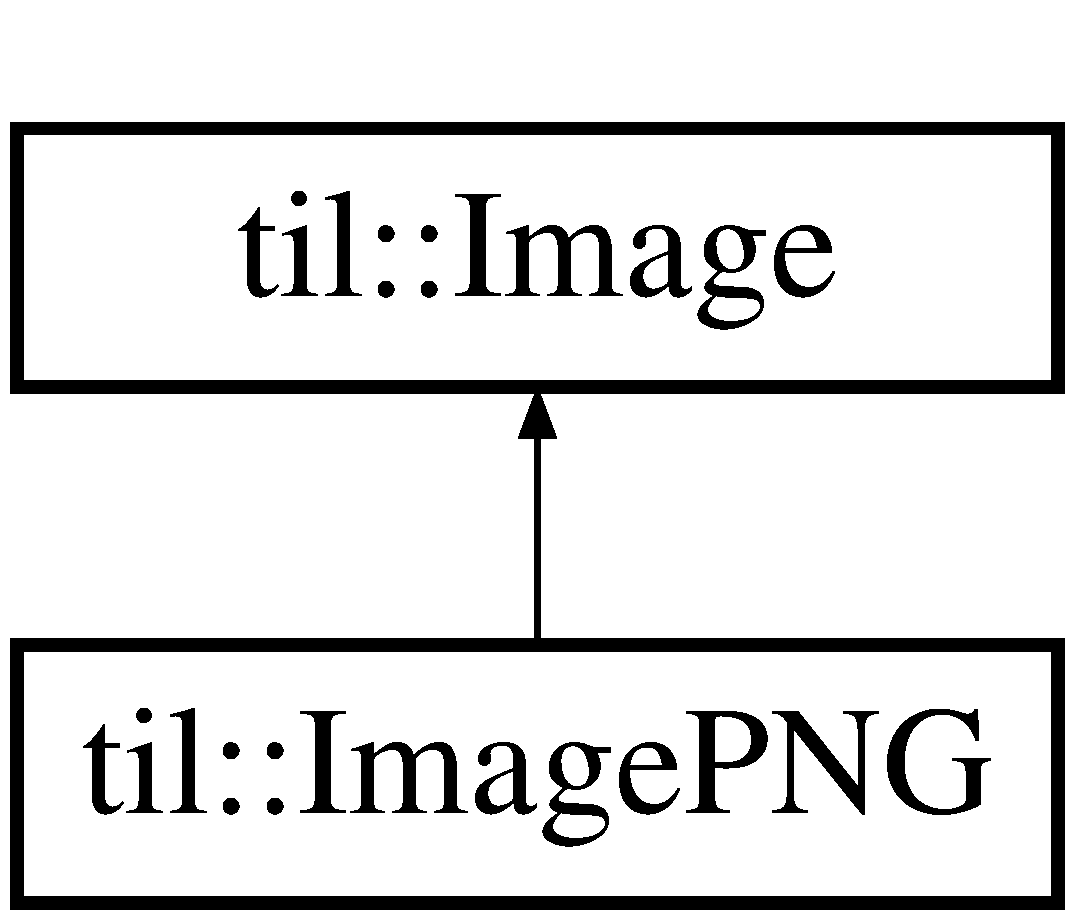
\includegraphics[height=2.000000cm]{classtil_1_1_image_p_n_g}
\end{center}
\end{figure}
\subsection*{Public Member Functions}
\begin{DoxyCompactItemize}
\item 
bool \hyperlink{classtil_1_1_image_p_n_g_aa3b8117c35f399d958870e3ecba9e1b7}{Parse} (\hyperlink{namespacetil_a20db61688ed403d11f057a508d87e54c}{uint32} a\_\-ColorDepth)
\begin{DoxyCompactList}\small\item\em Parses the actual image data. \item\end{DoxyCompactList}\item 
\hyperlink{namespacetil_a20db61688ed403d11f057a508d87e54c}{uint32} \hyperlink{classtil_1_1_image_p_n_g_a25dffae4745e88dab32c8dc7cdf3c591}{GetWidth} (\hyperlink{namespacetil_a20db61688ed403d11f057a508d87e54c}{uint32} a\_\-Frame=0)
\begin{DoxyCompactList}\small\item\em Get the width of a frame. \item\end{DoxyCompactList}\item 
\hyperlink{namespacetil_a20db61688ed403d11f057a508d87e54c}{uint32} \hyperlink{classtil_1_1_image_p_n_g_a64dff92207203a4673290a0ed3634538}{GetHeight} (\hyperlink{namespacetil_a20db61688ed403d11f057a508d87e54c}{uint32} a\_\-Frame=0)
\begin{DoxyCompactList}\small\item\em Get the height of a frame. \item\end{DoxyCompactList}\item 
\hyperlink{namespacetil_a20db61688ed403d11f057a508d87e54c}{uint32} \hyperlink{classtil_1_1_image_p_n_g_ade57a800697abe8f024a305e236b3471}{GetFrameCount} ()
\begin{DoxyCompactList}\small\item\em Returns the amount of frames this image contains. \item\end{DoxyCompactList}\item 
\hyperlink{namespacetil_a5f3ec10aca1a788b495a0bd3787bc2dc}{byte} $\ast$ \hyperlink{classtil_1_1_image_p_n_g_a2dc5b02cc0e64d2cf44202122c3e7e86}{GetPixels} (\hyperlink{namespacetil_a20db61688ed403d11f057a508d87e54c}{uint32} a\_\-Frame=0)
\begin{DoxyCompactList}\small\item\em Get the pixel data from this image. \item\end{DoxyCompactList}\end{DoxyCompactItemize}
\begin{Indent}{\bf Internal}\par
{\em These functions are internal and shouldn't be called by developers. }\begin{DoxyCompactItemize}
\item 
\hypertarget{classtil_1_1_image_p_n_g_acfdc45ec9a5a6e20e510290137619aaa}{
\hyperlink{namespacetil_a5f3ec10aca1a788b495a0bd3787bc2dc}{byte} {\bfseries GetByte} ()}
\label{classtil_1_1_image_p_n_g_acfdc45ec9a5a6e20e510290137619aaa}

\item 
\hypertarget{classtil_1_1_image_p_n_g_a34b1fec95bc2360726a037cfda20f799}{
\hyperlink{namespacetil_a7903a6761ac6f7472530b2863401909e}{word} {\bfseries GetWord} ()}
\label{classtil_1_1_image_p_n_g_a34b1fec95bc2360726a037cfda20f799}

\item 
\hypertarget{classtil_1_1_image_p_n_g_abc518dbfc7db53aac8671e1479330789}{
\hyperlink{namespacetil_a9babb870ec6cf9716ed0c90ea12811af}{dword} {\bfseries GetDWord} ()}
\label{classtil_1_1_image_p_n_g_abc518dbfc7db53aac8671e1479330789}

\item 
\hypertarget{classtil_1_1_image_p_n_g_a6c7242e1c3b0082aa5ece3960d560b71}{
void {\bfseries Skip} (\hyperlink{namespacetil_a20db61688ed403d11f057a508d87e54c}{uint32} a\_\-Bytes)}
\label{classtil_1_1_image_p_n_g_a6c7242e1c3b0082aa5ece3960d560b71}

\item 
\hypertarget{classtil_1_1_image_p_n_g_a69775247104a119080ec361277bfe70d}{
chunk $\ast$ {\bfseries GetChunkHeader} ()}
\label{classtil_1_1_image_p_n_g_a69775247104a119080ec361277bfe70d}

\item 
\hypertarget{classtil_1_1_image_p_n_g_ad74bd9c2b9d1e67f3474d4536a3c152f}{
bool {\bfseries Compile} ()}
\label{classtil_1_1_image_p_n_g_ad74bd9c2b9d1e67f3474d4536a3c152f}

\item 
\hypertarget{classtil_1_1_image_p_n_g_a54ee8d423351230d5a70177f29ec09e8}{
bool {\bfseries Compose} ()}
\label{classtil_1_1_image_p_n_g_a54ee8d423351230d5a70177f29ec09e8}

\end{DoxyCompactItemize}
\end{Indent}


\subsection{Detailed Description}
\hyperlink{classtil_1_1_image}{til::Image} implementation of a PNG loader. 

\subsection{Member Function Documentation}
\hypertarget{classtil_1_1_image_p_n_g_ade57a800697abe8f024a305e236b3471}{
\index{til::ImagePNG@{til::ImagePNG}!GetFrameCount@{GetFrameCount}}
\index{GetFrameCount@{GetFrameCount}!til::ImagePNG@{til::ImagePNG}}
\subsubsection[{GetFrameCount}]{\setlength{\rightskip}{0pt plus 5cm}{\bf uint32} til::ImagePNG::GetFrameCount (
\begin{DoxyParamCaption}
{}
\end{DoxyParamCaption}
)\hspace{0.3cm}{\ttfamily  \mbox{[}virtual\mbox{]}}}}
\label{classtil_1_1_image_p_n_g_ade57a800697abe8f024a305e236b3471}


Returns the amount of frames this image contains. 

Used when dealing with formats that support animation or multiple images.

\begin{DoxyNote}{Note}
There is never going to be support for other video formats. This is because TinyImageLoader is an $\ast$image$\ast$ loader, not a video loader. The exception to the rule are GIF89 and APNG, because it concerns an extension to a normally single-\/framed format. 
\end{DoxyNote}


Reimplemented from \hyperlink{classtil_1_1_image_a78c10e07b535c99840b0afd5aa165df4}{til::Image}.

\hypertarget{classtil_1_1_image_p_n_g_a64dff92207203a4673290a0ed3634538}{
\index{til::ImagePNG@{til::ImagePNG}!GetHeight@{GetHeight}}
\index{GetHeight@{GetHeight}!til::ImagePNG@{til::ImagePNG}}
\subsubsection[{GetHeight}]{\setlength{\rightskip}{0pt plus 5cm}{\bf uint32} til::ImagePNG::GetHeight (
\begin{DoxyParamCaption}
\item[{{\bf uint32}}]{a\_\-Frame = {\ttfamily 0}}
\end{DoxyParamCaption}
)\hspace{0.3cm}{\ttfamily  \mbox{[}virtual\mbox{]}}}}
\label{classtil_1_1_image_p_n_g_a64dff92207203a4673290a0ed3634538}


Get the height of a frame. 


\begin{DoxyParams}{Parameters}
{\em a\_\-Frame} & The frame of an animation or image to return.\\
\hline
\end{DoxyParams}
\begin{DoxyReturn}{Returns}
The height as a uint32.
\end{DoxyReturn}
Some formats support multiple frames or images with different dimensions. You can call this function with a frame number to get the correct dimensions. 

Implements \hyperlink{classtil_1_1_image_ad623add911ba5230f56a4cc58af75ec1}{til::Image}.

\hypertarget{classtil_1_1_image_p_n_g_a2dc5b02cc0e64d2cf44202122c3e7e86}{
\index{til::ImagePNG@{til::ImagePNG}!GetPixels@{GetPixels}}
\index{GetPixels@{GetPixels}!til::ImagePNG@{til::ImagePNG}}
\subsubsection[{GetPixels}]{\setlength{\rightskip}{0pt plus 5cm}{\bf byte}$\ast$ til::ImagePNG::GetPixels (
\begin{DoxyParamCaption}
\item[{{\bf uint32}}]{a\_\-Frame = {\ttfamily 0}}
\end{DoxyParamCaption}
)\hspace{0.3cm}{\ttfamily  \mbox{[}virtual\mbox{]}}}}
\label{classtil_1_1_image_p_n_g_a2dc5b02cc0e64d2cf44202122c3e7e86}


Get the pixel data from this image. 


\begin{DoxyParams}{Parameters}
{\em a\_\-Frame} & The frame of an animation to return.\\
\hline
\end{DoxyParams}
\begin{DoxyReturn}{Returns}
Pixel array as a byte array.
\end{DoxyReturn}
The data is encoded according to the color depth specified. For instance, when loading images as 32-\/bit ARGB, the stream of bytes must be converted to unsigned long before being used.


\begin{DoxyCode}
                        til::Image* load = TIL_Load("media\\texture.png", 
      TIL_DEPTH_A8B8G8R8 | TIL_FILE_ADDWORKINGDIR);
                        unsigned long* pixels = (unsigned long*)load->GetPixels()
      ;
\end{DoxyCode}
 

Implements \hyperlink{classtil_1_1_image_a8dd46f6477025e23dc921e1a4a3f6a62}{til::Image}.

\hypertarget{classtil_1_1_image_p_n_g_a25dffae4745e88dab32c8dc7cdf3c591}{
\index{til::ImagePNG@{til::ImagePNG}!GetWidth@{GetWidth}}
\index{GetWidth@{GetWidth}!til::ImagePNG@{til::ImagePNG}}
\subsubsection[{GetWidth}]{\setlength{\rightskip}{0pt plus 5cm}{\bf uint32} til::ImagePNG::GetWidth (
\begin{DoxyParamCaption}
\item[{{\bf uint32}}]{a\_\-Frame = {\ttfamily 0}}
\end{DoxyParamCaption}
)\hspace{0.3cm}{\ttfamily  \mbox{[}virtual\mbox{]}}}}
\label{classtil_1_1_image_p_n_g_a25dffae4745e88dab32c8dc7cdf3c591}


Get the width of a frame. 


\begin{DoxyParams}{Parameters}
{\em a\_\-Frame} & The frame of an animation or image to return.\\
\hline
\end{DoxyParams}
\begin{DoxyReturn}{Returns}
The width as a uint32.
\end{DoxyReturn}
Some formats support multiple frames or images with different dimensions. You can call this function with a frame number to get the correct dimensions. 

Implements \hyperlink{classtil_1_1_image_a769be7e5a2cc490e8ae70b7c29a56eca}{til::Image}.

\hypertarget{classtil_1_1_image_p_n_g_aa3b8117c35f399d958870e3ecba9e1b7}{
\index{til::ImagePNG@{til::ImagePNG}!Parse@{Parse}}
\index{Parse@{Parse}!til::ImagePNG@{til::ImagePNG}}
\subsubsection[{Parse}]{\setlength{\rightskip}{0pt plus 5cm}bool til::ImagePNG::Parse (
\begin{DoxyParamCaption}
\item[{{\bf uint32}}]{a\_\-ColorDepth}
\end{DoxyParamCaption}
)\hspace{0.3cm}{\ttfamily  \mbox{[}virtual\mbox{]}}}}
\label{classtil_1_1_image_p_n_g_aa3b8117c35f399d958870e3ecba9e1b7}


Parses the actual image data. 


\begin{DoxyParams}{Parameters}
{\em a\_\-ColorDepth} & The color depth received from \hyperlink{classtil_1_1_image_ae1202f84c0addb81eba161f746a9d4cc}{SetBPP};\\
\hline
\end{DoxyParams}
This method is pure virtual and should be overwritten by an image loading implementation. 

Implements \hyperlink{classtil_1_1_image_a2436c982f6b403ab07591f06107fe432}{til::Image}.



The documentation for this class was generated from the following file:\begin{DoxyCompactItemize}
\item 
SDK/headers/\hyperlink{_t_i_l_image_p_n_g_8h}{TILImagePNG.h}\end{DoxyCompactItemize}

\hypertarget{classtil_1_1_image_t_g_a}{
\section{til::ImageTGA Class Reference}
\label{classtil_1_1_image_t_g_a}\index{til::ImageTGA@{til::ImageTGA}}
}


\hyperlink{classtil_1_1_image}{til::Image} implementation of a TGA loader.  




{\ttfamily \#include $<$TILImageTGA.h$>$}

Inheritance diagram for til::ImageTGA:\begin{figure}[H]
\begin{center}
\leavevmode
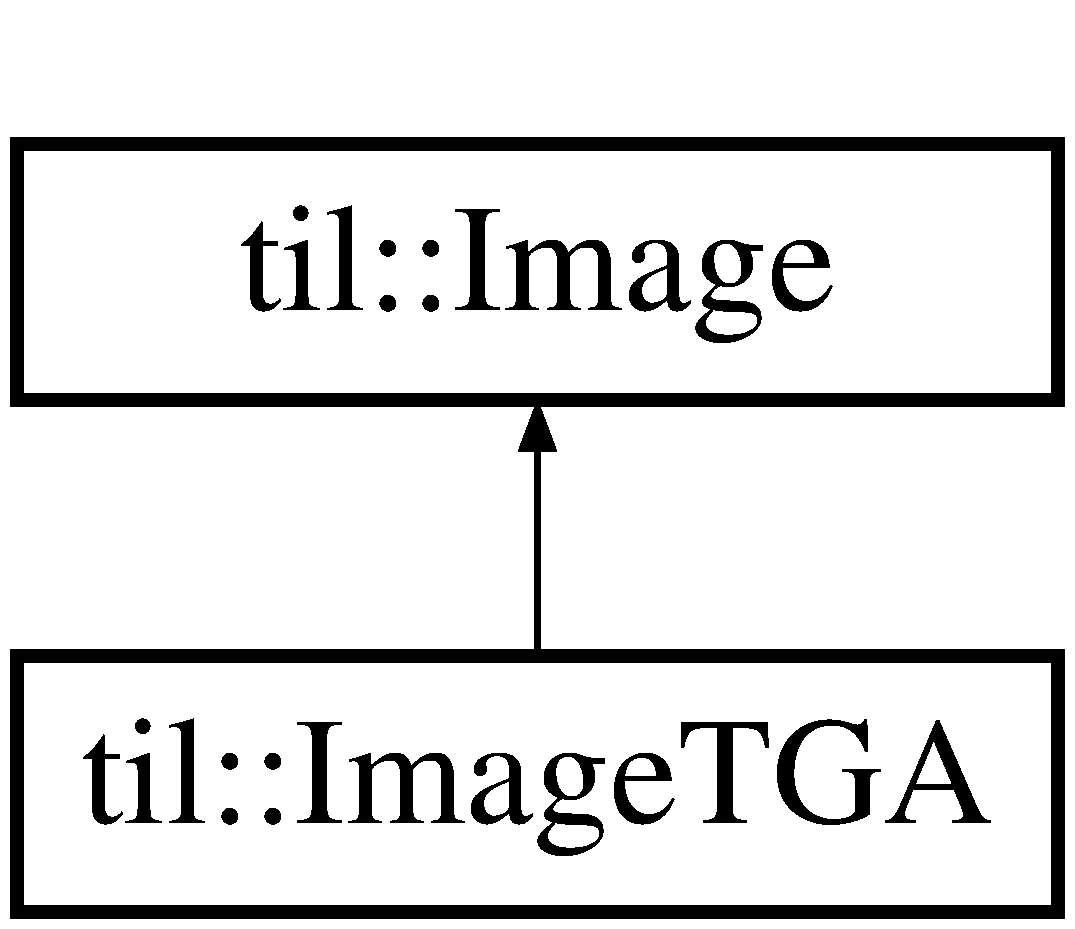
\includegraphics[height=2.000000cm]{classtil_1_1_image_t_g_a}
\end{center}
\end{figure}
\subsection*{Public Member Functions}
\begin{DoxyCompactItemize}
\item 
bool \hyperlink{classtil_1_1_image_t_g_a_a283c391e9d3709b974ebca14d5eb2ebd}{Parse} (\hyperlink{namespacetil_a20db61688ed403d11f057a508d87e54c}{uint32} a\_\-ColorDepth)
\begin{DoxyCompactList}\small\item\em Parses the actual image data. \item\end{DoxyCompactList}\item 
\hyperlink{namespacetil_a20db61688ed403d11f057a508d87e54c}{uint32} \hyperlink{classtil_1_1_image_t_g_a_a46d1df102d6125290c6bba65a3ed9814}{GetFrameCount} ()
\begin{DoxyCompactList}\small\item\em Returns the amount of frames this image contains. \item\end{DoxyCompactList}\item 
\hyperlink{namespacetil_a5f3ec10aca1a788b495a0bd3787bc2dc}{byte} $\ast$ \hyperlink{classtil_1_1_image_t_g_a_a5202d714441c2df497368905bd4c5b83}{GetPixels} (\hyperlink{namespacetil_a20db61688ed403d11f057a508d87e54c}{uint32} a\_\-Frame=0)
\begin{DoxyCompactList}\small\item\em Get the pixel data from this image. \item\end{DoxyCompactList}\item 
\hyperlink{namespacetil_a20db61688ed403d11f057a508d87e54c}{uint32} \hyperlink{classtil_1_1_image_t_g_a_a760434c274b1ea02e9c23ba1c618da84}{GetWidth} (\hyperlink{namespacetil_a20db61688ed403d11f057a508d87e54c}{uint32} a\_\-Frame=0)
\begin{DoxyCompactList}\small\item\em Get the width of a frame. \item\end{DoxyCompactList}\item 
\hyperlink{namespacetil_a20db61688ed403d11f057a508d87e54c}{uint32} \hyperlink{classtil_1_1_image_t_g_a_a4284b8576ce42b239beec36bd6902eac}{GetHeight} (\hyperlink{namespacetil_a20db61688ed403d11f057a508d87e54c}{uint32} a\_\-Frame=0)
\begin{DoxyCompactList}\small\item\em Get the height of a frame. \item\end{DoxyCompactList}\end{DoxyCompactItemize}
\begin{Indent}{\bf Internal}\par
{\em These functions are internal and shouldn't be called by developers. }\begin{DoxyCompactItemize}
\item 
\hypertarget{classtil_1_1_image_t_g_a_a1c911720ba5cc530a0fcf18568de6d0e}{
bool \hyperlink{classtil_1_1_image_t_g_a_a1c911720ba5cc530a0fcf18568de6d0e}{CompileUncompressed} ()}
\label{classtil_1_1_image_t_g_a_a1c911720ba5cc530a0fcf18568de6d0e}

\begin{DoxyCompactList}\small\item\em Compile uncompressed image data to pixel information. \item\end{DoxyCompactList}\item 
\hypertarget{classtil_1_1_image_t_g_a_ae553d660c08f8f544fb472c5f5b13d64}{
bool \hyperlink{classtil_1_1_image_t_g_a_ae553d660c08f8f544fb472c5f5b13d64}{CompileRunLengthEncoded} ()}
\label{classtil_1_1_image_t_g_a_ae553d660c08f8f544fb472c5f5b13d64}

\begin{DoxyCompactList}\small\item\em Compile compressed image data to pixel information. \item\end{DoxyCompactList}\end{DoxyCompactItemize}
\end{Indent}


\subsection{Detailed Description}
\hyperlink{classtil_1_1_image}{til::Image} implementation of a TGA loader. 

\subsection{Member Function Documentation}
\hypertarget{classtil_1_1_image_t_g_a_a46d1df102d6125290c6bba65a3ed9814}{
\index{til::ImageTGA@{til::ImageTGA}!GetFrameCount@{GetFrameCount}}
\index{GetFrameCount@{GetFrameCount}!til::ImageTGA@{til::ImageTGA}}
\subsubsection[{GetFrameCount}]{\setlength{\rightskip}{0pt plus 5cm}{\bf uint32} til::ImageTGA::GetFrameCount (
\begin{DoxyParamCaption}
{}
\end{DoxyParamCaption}
)\hspace{0.3cm}{\ttfamily  \mbox{[}virtual\mbox{]}}}}
\label{classtil_1_1_image_t_g_a_a46d1df102d6125290c6bba65a3ed9814}


Returns the amount of frames this image contains. 

Used when dealing with formats that support animation or multiple images.

\begin{DoxyNote}{Note}
There is never going to be support for other video formats. This is because TinyImageLoader is an $\ast$image$\ast$ loader, not a video loader. The exception to the rule are GIF89 and APNG, because it concerns an extension to a normally single-\/framed format. 
\end{DoxyNote}


Reimplemented from \hyperlink{classtil_1_1_image_a78c10e07b535c99840b0afd5aa165df4}{til::Image}.

\hypertarget{classtil_1_1_image_t_g_a_a4284b8576ce42b239beec36bd6902eac}{
\index{til::ImageTGA@{til::ImageTGA}!GetHeight@{GetHeight}}
\index{GetHeight@{GetHeight}!til::ImageTGA@{til::ImageTGA}}
\subsubsection[{GetHeight}]{\setlength{\rightskip}{0pt plus 5cm}{\bf uint32} til::ImageTGA::GetHeight (
\begin{DoxyParamCaption}
\item[{{\bf uint32}}]{a\_\-Frame = {\ttfamily 0}}
\end{DoxyParamCaption}
)\hspace{0.3cm}{\ttfamily  \mbox{[}virtual\mbox{]}}}}
\label{classtil_1_1_image_t_g_a_a4284b8576ce42b239beec36bd6902eac}


Get the height of a frame. 


\begin{DoxyParams}{Parameters}
{\em a\_\-Frame} & The frame of an animation or image to return.\\
\hline
\end{DoxyParams}
\begin{DoxyReturn}{Returns}
The height as a uint32.
\end{DoxyReturn}
Some formats support multiple frames or images with different dimensions. You can call this function with a frame number to get the correct dimensions. 

Implements \hyperlink{classtil_1_1_image_ad623add911ba5230f56a4cc58af75ec1}{til::Image}.

\hypertarget{classtil_1_1_image_t_g_a_a5202d714441c2df497368905bd4c5b83}{
\index{til::ImageTGA@{til::ImageTGA}!GetPixels@{GetPixels}}
\index{GetPixels@{GetPixels}!til::ImageTGA@{til::ImageTGA}}
\subsubsection[{GetPixels}]{\setlength{\rightskip}{0pt plus 5cm}{\bf byte}$\ast$ til::ImageTGA::GetPixels (
\begin{DoxyParamCaption}
\item[{{\bf uint32}}]{a\_\-Frame = {\ttfamily 0}}
\end{DoxyParamCaption}
)\hspace{0.3cm}{\ttfamily  \mbox{[}virtual\mbox{]}}}}
\label{classtil_1_1_image_t_g_a_a5202d714441c2df497368905bd4c5b83}


Get the pixel data from this image. 


\begin{DoxyParams}{Parameters}
{\em a\_\-Frame} & The frame of an animation to return.\\
\hline
\end{DoxyParams}
\begin{DoxyReturn}{Returns}
Pixel array as a byte array.
\end{DoxyReturn}
The data is encoded according to the color depth specified. For instance, when loading images as 32-\/bit ARGB, the stream of bytes must be converted to unsigned long before being used.


\begin{DoxyCode}
                        til::Image* load = TIL_Load("media\\texture.png", 
      TIL_DEPTH_A8B8G8R8 | TIL_FILE_ADDWORKINGDIR);
                        unsigned long* pixels = (unsigned long*)load->GetPixels()
      ;
\end{DoxyCode}
 

Implements \hyperlink{classtil_1_1_image_a8dd46f6477025e23dc921e1a4a3f6a62}{til::Image}.

\hypertarget{classtil_1_1_image_t_g_a_a760434c274b1ea02e9c23ba1c618da84}{
\index{til::ImageTGA@{til::ImageTGA}!GetWidth@{GetWidth}}
\index{GetWidth@{GetWidth}!til::ImageTGA@{til::ImageTGA}}
\subsubsection[{GetWidth}]{\setlength{\rightskip}{0pt plus 5cm}{\bf uint32} til::ImageTGA::GetWidth (
\begin{DoxyParamCaption}
\item[{{\bf uint32}}]{a\_\-Frame = {\ttfamily 0}}
\end{DoxyParamCaption}
)\hspace{0.3cm}{\ttfamily  \mbox{[}virtual\mbox{]}}}}
\label{classtil_1_1_image_t_g_a_a760434c274b1ea02e9c23ba1c618da84}


Get the width of a frame. 


\begin{DoxyParams}{Parameters}
{\em a\_\-Frame} & The frame of an animation or image to return.\\
\hline
\end{DoxyParams}
\begin{DoxyReturn}{Returns}
The width as a uint32.
\end{DoxyReturn}
Some formats support multiple frames or images with different dimensions. You can call this function with a frame number to get the correct dimensions. 

Implements \hyperlink{classtil_1_1_image_a769be7e5a2cc490e8ae70b7c29a56eca}{til::Image}.

\hypertarget{classtil_1_1_image_t_g_a_a283c391e9d3709b974ebca14d5eb2ebd}{
\index{til::ImageTGA@{til::ImageTGA}!Parse@{Parse}}
\index{Parse@{Parse}!til::ImageTGA@{til::ImageTGA}}
\subsubsection[{Parse}]{\setlength{\rightskip}{0pt plus 5cm}bool til::ImageTGA::Parse (
\begin{DoxyParamCaption}
\item[{{\bf uint32}}]{a\_\-ColorDepth}
\end{DoxyParamCaption}
)\hspace{0.3cm}{\ttfamily  \mbox{[}virtual\mbox{]}}}}
\label{classtil_1_1_image_t_g_a_a283c391e9d3709b974ebca14d5eb2ebd}


Parses the actual image data. 


\begin{DoxyParams}{Parameters}
{\em a\_\-ColorDepth} & The color depth received from \hyperlink{classtil_1_1_image_ae1202f84c0addb81eba161f746a9d4cc}{SetBPP};\\
\hline
\end{DoxyParams}
This method is pure virtual and should be overwritten by an image loading implementation. 

Implements \hyperlink{classtil_1_1_image_a2436c982f6b403ab07591f06107fe432}{til::Image}.



The documentation for this class was generated from the following file:\begin{DoxyCompactItemize}
\item 
SDK/headers/\hyperlink{_t_i_l_image_t_g_a_8h}{TILImageTGA.h}\end{DoxyCompactItemize}

\hypertarget{structtil_1_1_message_data}{
\section{til::MessageData Struct Reference}
\label{structtil_1_1_message_data}\index{til::MessageData@{til::MessageData}}
}


Message structure.  




{\ttfamily \#include $<$TILSettings.h$>$}

\subsection*{Public Attributes}
\begin{DoxyCompactItemize}
\item 
char $\ast$ \hyperlink{structtil_1_1_message_data_a509ca54f8bbc534d0220d3e7b1637a8d}{message}
\item 
char $\ast$ \hyperlink{structtil_1_1_message_data_a0e06be68ecffce75b5920a24d367bad7}{source\_\-file}
\item 
int \hyperlink{structtil_1_1_message_data_a431af7e6298fbf1d6a0cf4518d67d153}{source\_\-line}
\end{DoxyCompactItemize}


\subsection{Detailed Description}
Message structure. 

\subsection{Member Data Documentation}
\hypertarget{structtil_1_1_message_data_a509ca54f8bbc534d0220d3e7b1637a8d}{
\index{til::MessageData@{til::MessageData}!message@{message}}
\index{message@{message}!til::MessageData@{til::MessageData}}
\subsubsection[{message}]{\setlength{\rightskip}{0pt plus 5cm}char$\ast$ {\bf til::MessageData::message}}}
\label{structtil_1_1_message_data_a509ca54f8bbc534d0220d3e7b1637a8d}
Contains the message provided by TinyImageLoader. \hypertarget{structtil_1_1_message_data_a0e06be68ecffce75b5920a24d367bad7}{
\index{til::MessageData@{til::MessageData}!source\_\-file@{source\_\-file}}
\index{source\_\-file@{source\_\-file}!til::MessageData@{til::MessageData}}
\subsubsection[{source\_\-file}]{\setlength{\rightskip}{0pt plus 5cm}char$\ast$ {\bf til::MessageData::source\_\-file}}}
\label{structtil_1_1_message_data_a0e06be68ecffce75b5920a24d367bad7}
The file where the message originated. \hypertarget{structtil_1_1_message_data_a431af7e6298fbf1d6a0cf4518d67d153}{
\index{til::MessageData@{til::MessageData}!source\_\-line@{source\_\-line}}
\index{source\_\-line@{source\_\-line}!til::MessageData@{til::MessageData}}
\subsubsection[{source\_\-line}]{\setlength{\rightskip}{0pt plus 5cm}int {\bf til::MessageData::source\_\-line}}}
\label{structtil_1_1_message_data_a431af7e6298fbf1d6a0cf4518d67d153}
The line the message came from. 

The documentation for this struct was generated from the following file:\begin{DoxyCompactItemize}
\item 
SDK/headers/\hyperlink{_t_i_l_settings_8h}{TILSettings.h}\end{DoxyCompactItemize}

\chapter{File Documentation}
\hypertarget{example-opengl-texture_8cpp}{
\section{examples/src/example-\/opengl-\/texture.cpp File Reference}
\label{example-opengl-texture_8cpp}\index{examples/src/example-\/opengl-\/texture.cpp@{examples/src/example-\/opengl-\/texture.cpp}}
}
{\ttfamily \#include \char`\"{}Framework.h\char`\"{}}\par
{\ttfamily \#include \char`\"{}TinyImageLoader.h\char`\"{}}\par
\subsection*{Namespaces}
\begin{DoxyCompactItemize}
\item 
namespace \hyperlink{namespace_t_i_l_f_w}{TILFW}


\begin{DoxyCompactList}\small\item\em TinyImageLoader \hyperlink{class_t_i_l_f_w_1_1_framework}{Framework} namespace. \item\end{DoxyCompactList}

\end{DoxyCompactItemize}
\subsection*{Variables}
\begin{DoxyCompactItemize}
\item 
\hypertarget{namespace_t_i_l_f_w_a5a6b9c19ed6a42d133f77a0897579243}{
D {\bfseries TILFW::\_\-\_\-pad0\_\-\_\-}}
\label{namespace_t_i_l_f_w_a5a6b9c19ed6a42d133f77a0897579243}

\item 
\hypertarget{namespace_t_i_l_f_w_a74d9924a1a473f0ff11e69da582501ec}{
{\bfseries TILFW::s\_\-WindowHeight} = 480}
\label{namespace_t_i_l_f_w_a74d9924a1a473f0ff11e69da582501ec}

\end{DoxyCompactItemize}


\subsection{Detailed Description}

\hypertarget{example-zip-loading_8cpp}{
\section{examples/src/example-\/zip-\/loading.cpp File Reference}
\label{example-zip-loading_8cpp}\index{examples/src/example-\/zip-\/loading.cpp@{examples/src/example-\/zip-\/loading.cpp}}
}
{\ttfamily \#include \char`\"{}Framework.h\char`\"{}}\par
{\ttfamily \#include \char`\"{}TinyImageLoader.h\char`\"{}}\par


\subsection{Detailed Description}

\hypertarget{_framework_8h}{
\section{examples/src/Framework.h File Reference}
\label{_framework_8h}\index{examples/src/Framework.h@{examples/src/Framework.h}}
}
{\ttfamily \#include $<$stdio.h$>$}\par
{\ttfamily \#include $<$windows.h$>$}\par
{\ttfamily \#include \char`\"{}GL/glew.h\char`\"{}}\par
{\ttfamily \#include \char`\"{}GL/gl.h\char`\"{}}\par
{\ttfamily \#include \char`\"{}GL/wglew.h\char`\"{}}\par
{\ttfamily \#include \char`\"{}GL/glext.h\char`\"{}}\par
{\ttfamily \#include \char`\"{}GL/wglext.h\char`\"{}}\par
\subsection*{Classes}
\begin{DoxyCompactItemize}
\item 
class \hyperlink{class_t_i_l_f_w_1_1_framework}{TILFW::Framework}
\end{DoxyCompactItemize}
\subsection*{Namespaces}
\begin{DoxyCompactItemize}
\item 
namespace \hyperlink{namespace_t_i_l_f_w}{TILFW}


\begin{DoxyCompactList}\small\item\em TinyImageLoader \hyperlink{class_t_i_l_f_w_1_1_framework}{Framework} namespace. \item\end{DoxyCompactList}

\end{DoxyCompactItemize}


\subsection{Detailed Description}

\hypertarget{_t_i_l_colors_8h}{
\section{SDK/headers/TILColors.h File Reference}
\label{_t_i_l_colors_8h}\index{SDK/headers/TILColors.h@{SDK/headers/TILColors.h}}
}


Functions for constructing colors, converting colors and blending colors.  


{\ttfamily \#include \char`\"{}TILSettings.h\char`\"{}}\par
\subsection*{Namespaces}
\begin{DoxyCompactItemize}
\item 
namespace \hyperlink{namespacetil}{til}


\begin{DoxyCompactList}\small\item\em TinyImageLoader namespace. \item\end{DoxyCompactList}

\end{DoxyCompactItemize}
\subsection*{Functions}
\begin{Indent}{\bf 16-\/bit RGB}\par
\begin{DoxyCompactItemize}
\item 
color\_\-16b \hyperlink{namespacetil_a7e42efe1f69a94e67190c1434fd002f4}{til::Construct\_\-16b\_\-R5G6B5} (uint8 a\_\-Red, uint8 a\_\-Green, uint8 a\_\-Blue)
\begin{DoxyCompactList}\small\item\em Construct a 16-\/bit RGB color. \item\end{DoxyCompactList}\item 
color\_\-16b \hyperlink{namespacetil_aa272abfc1060298455205cfe08c95e37}{til::AlphaBlend\_\-16b\_\-R5G6B5} (uint8 a\_\-Red, uint8 a\_\-Green, uint8 a\_\-Blue, uint8 a\_\-Alpha)
\begin{DoxyCompactList}\small\item\em Alpha blend a 16-\/bit RGB color. \item\end{DoxyCompactList}\item 
color\_\-16b \hyperlink{namespacetil_a1644b5f4cb28c7d3bc752873b66d3f58}{til::Blend\_\-16b\_\-R5G6B5} (color\_\-16b a\_\-Left, color\_\-16b a\_\-Right, uint8 a\_\-Factor)
\begin{DoxyCompactList}\small\item\em Blend between two 16-\/bit RGB colors. \item\end{DoxyCompactList}\item 
color\_\-32b \hyperlink{namespacetil_a2c7206c211d1a546b6ceb3e1170efd54}{til::Convert\_\-From\_\-16b\_\-R5G6B5\_\-To\_\-32b\_\-A8R8G8B8} (color\_\-16b a\_\-Color)
\begin{DoxyCompactList}\small\item\em Convert a 16-\/bit RGB color to a 32-\/bit ARGB color. \item\end{DoxyCompactList}\item 
color\_\-32b \hyperlink{namespacetil_a136075678006abfa91e534eeb9049f9c}{til::Convert\_\-From\_\-16b\_\-R5G6B5\_\-To\_\-32b\_\-A8B8G8R8} (color\_\-16b a\_\-Color)
\begin{DoxyCompactList}\small\item\em Convert a 16-\/bit RGB color to a 32-\/bit ABGR color. \item\end{DoxyCompactList}\end{DoxyCompactItemize}
\end{Indent}
\begin{Indent}{\bf 16-\/bit BGR}\par
\begin{DoxyCompactItemize}
\item 
color\_\-16b \hyperlink{namespacetil_accd82fcffbc0f256c971beb941ab9166}{til::Construct\_\-16b\_\-B5G6R5} (uint8 a\_\-Red, uint8 a\_\-Green, uint8 a\_\-Blue)
\begin{DoxyCompactList}\small\item\em Construct a 16-\/bit BGR color. \item\end{DoxyCompactList}\item 
color\_\-16b \hyperlink{namespacetil_a7db23332b0b6b0922c591645e418d3f1}{til::Blend\_\-16b\_\-B5G6R5} (color\_\-16b a\_\-Left, color\_\-16b a\_\-Right, uint8 a\_\-Factor)
\begin{DoxyCompactList}\small\item\em Blend between two 16-\/bit BGR colors. \item\end{DoxyCompactList}\item 
color\_\-32b \hyperlink{namespacetil_ae0e2e24eaa0772d2ca196be6cf18b2b8}{til::Convert\_\-From\_\-16b\_\-B5G6R5\_\-To\_\-32b\_\-A8R8G8B8} (color\_\-16b a\_\-Color)
\begin{DoxyCompactList}\small\item\em Convert a 16-\/bit BGR color to a 32-\/bit ARGB color. \item\end{DoxyCompactList}\item 
color\_\-32b \hyperlink{namespacetil_aefd9e893058049b916052a7325c827ba}{til::Convert\_\-From\_\-16b\_\-B5G6R5\_\-To\_\-32b\_\-A8B8G8R8} (color\_\-16b a\_\-Color)
\begin{DoxyCompactList}\small\item\em Convert a 16-\/bit BGR color to a 32-\/bit ABGR color. \item\end{DoxyCompactList}\end{DoxyCompactItemize}
\end{Indent}
\begin{Indent}{\bf 32-\/bit RGB}\par
\begin{DoxyCompactItemize}
\item 
color\_\-32b \hyperlink{namespacetil_ab7e7028c4a3c92cdca1a7b6dbf1c12bc}{til::Construct\_\-32b\_\-R8G8B8} (uint8 a\_\-Red, uint8 a\_\-Green, uint8 a\_\-Blue, uint8 a\_\-Alpha=0)
\begin{DoxyCompactList}\small\item\em Construct a 32-\/bit RGB color. \item\end{DoxyCompactList}\item 
color\_\-32b \hyperlink{namespacetil_afdfe84791f3958a513026bd931448eab}{til::AlphaBlend\_\-32b\_\-R8G8B8} (color\_\-32b a\_\-Color, uint8 a\_\-Amount)
\begin{DoxyCompactList}\small\item\em Alpha blend a 32-\/bit RGB color. \item\end{DoxyCompactList}\item 
color\_\-32b \hyperlink{namespacetil_aae7448d66a50340093fd0d7a17bc417d}{til::AlphaBlend\_\-32b\_\-R8G8B8} (uint8 a\_\-Red, uint8 a\_\-Green, uint8 a\_\-Blue, uint8 a\_\-Alpha)
\begin{DoxyCompactList}\small\item\em Alpha blend a 32-\/bit RGB color. \item\end{DoxyCompactList}\item 
color\_\-32b \hyperlink{namespacetil_ae4cb7b237e7e18881233e2230ce58cd5}{til::Blend\_\-32b\_\-R8G8B8} (color\_\-32b a\_\-Left, color\_\-32b a\_\-Right, uint8 a\_\-Factor)
\begin{DoxyCompactList}\small\item\em Blend between two 32-\/bit RGB colors. \item\end{DoxyCompactList}\end{DoxyCompactItemize}
\end{Indent}
\begin{Indent}{\bf 32-\/bit BGR}\par
\begin{DoxyCompactItemize}
\item 
color\_\-32b \hyperlink{namespacetil_ab3bc972471ad2a5739b7a3468c6fc5b7}{til::Construct\_\-32b\_\-B8G8R8} (uint8 a\_\-Red, uint8 a\_\-Green, uint8 a\_\-Blue, uint8 a\_\-Alpha=0)
\begin{DoxyCompactList}\small\item\em Construct a 32-\/bit BGR color. \item\end{DoxyCompactList}\item 
color\_\-32b \hyperlink{namespacetil_ad141ab11e843c3ad322d25bf38822cda}{til::AlphaBlend\_\-32b\_\-B8G8R8} (uint8 a\_\-Red, uint8 a\_\-Green, uint8 a\_\-Blue, uint8 a\_\-Alpha)
\begin{DoxyCompactList}\small\item\em Alpha blend a 32-\/bit BGR color. \item\end{DoxyCompactList}\end{DoxyCompactItemize}
\end{Indent}
\begin{Indent}{\bf 32-\/bit ARGB}\par
\begin{DoxyCompactItemize}
\item 
color\_\-32b \hyperlink{namespacetil_a9dc7ee813858f38308e7d38df21b0953}{til::Construct\_\-32b\_\-A8R8G8B8} (uint8 a\_\-Red, uint8 a\_\-Green, uint8 a\_\-Blue, uint8 a\_\-Alpha)
\begin{DoxyCompactList}\small\item\em Construct a 32-\/bit ARGB color. \item\end{DoxyCompactList}\item 
color\_\-32b \hyperlink{namespacetil_a269385b5e84783f03c13fc7a590b6a44}{til::Construct\_\-32b\_\-A8R8G8B8} (color\_\-32b a\_\-Color, uint8 a\_\-Alpha)
\begin{DoxyCompactList}\small\item\em Construct a 32-\/bit ARGB color. \item\end{DoxyCompactList}\item 
color\_\-32b \hyperlink{namespacetil_a1b2bc733875b4132b63390b24c3ccae1}{til::AlphaBlend\_\-32b\_\-A8R8G8B8} (uint8 a\_\-Red, uint8 a\_\-Green, uint8 a\_\-Blue, uint8 a\_\-Alpha)
\begin{DoxyCompactList}\small\item\em Alpha blend a 32-\/bit ARGB color. \item\end{DoxyCompactList}\end{DoxyCompactItemize}
\end{Indent}
\begin{Indent}{\bf 32-\/bit ABGR}\par
\begin{DoxyCompactItemize}
\item 
color\_\-32b \hyperlink{namespacetil_a9910d275ad1592463eb89634423d7110}{til::Construct\_\-32b\_\-A8B8G8R8} (uint8 a\_\-Red, uint8 a\_\-Green, uint8 a\_\-Blue, uint8 a\_\-Alpha)
\begin{DoxyCompactList}\small\item\em Construct a 32-\/bit ABGR color. \item\end{DoxyCompactList}\item 
color\_\-32b \hyperlink{namespacetil_a59b7c2ae7112fe3cff94e67826fca681}{til::Construct\_\-32b\_\-A8B8G8R8} (color\_\-32b a\_\-Color, uint8 a\_\-Alpha)
\begin{DoxyCompactList}\small\item\em Construct a 32-\/bit ABGR color. \item\end{DoxyCompactList}\item 
color\_\-32b \hyperlink{namespacetil_a1ff33e54fd1c245f093a779b13e9ec43}{til::AlphaBlend\_\-32b\_\-A8B8G8R8} (uint8 a\_\-Red, uint8 a\_\-Green, uint8 a\_\-Blue, uint8 a\_\-Alpha)
\begin{DoxyCompactList}\small\item\em Alpha blend a 32-\/bit ABGR color. \item\end{DoxyCompactList}\end{DoxyCompactItemize}
\end{Indent}
\begin{Indent}{\bf 32-\/bit RGBA}\par
\begin{DoxyCompactItemize}
\item 
color\_\-32b \hyperlink{namespacetil_ae14596c98e011e44e22c8cca0ddccc7e}{til::Construct\_\-32b\_\-R8G8B8A8} (uint8 a\_\-Red, uint8 a\_\-Green, uint8 a\_\-Blue, uint8 a\_\-Alpha)
\begin{DoxyCompactList}\small\item\em Construct a 32-\/bit RGBA color. \item\end{DoxyCompactList}\item 
color\_\-32b \hyperlink{namespacetil_af5177e6fa03dee2ef309469f0b72c7a8}{til::AlphaBlend\_\-32b\_\-R8G8B8A8} (uint8 a\_\-Red, uint8 a\_\-Green, uint8 a\_\-Blue, uint8 a\_\-Alpha)
\begin{DoxyCompactList}\small\item\em Alpha blend a 32-\/bit RGBA color. \item\end{DoxyCompactList}\end{DoxyCompactItemize}
\end{Indent}
\begin{Indent}{\bf 32-\/bit BGRA}\par
\begin{DoxyCompactItemize}
\item 
color\_\-32b \hyperlink{namespacetil_afb2e7b72d4fd06e3faf946558fab2c5e}{til::Construct\_\-32b\_\-B8G8R8A8} (uint8 a\_\-Red, uint8 a\_\-Green, uint8 a\_\-Blue, uint8 a\_\-Alpha)
\begin{DoxyCompactList}\small\item\em Construct a 32-\/bit BGRA color. \item\end{DoxyCompactList}\item 
color\_\-32b \hyperlink{namespacetil_a8e053d490a2c4f46f6a355896bbf7d89}{til::AlphaBlend\_\-32b\_\-B8G8R8A8} (uint8 a\_\-Red, uint8 a\_\-Green, uint8 a\_\-Blue, uint8 a\_\-Alpha)
\begin{DoxyCompactList}\small\item\em Alpha blend a 32-\/bit BGRA color. \item\end{DoxyCompactList}\end{DoxyCompactItemize}
\end{Indent}
\subsection*{Variables}
\begin{DoxyCompactItemize}
\item 
\hypertarget{namespacetil_affbd5605556e0eeb2d303fbb2d9b6092}{
D {\bfseries til::\_\-\_\-pad0\_\-\_\-}}
\label{namespacetil_affbd5605556e0eeb2d303fbb2d9b6092}

\end{DoxyCompactItemize}


\subsection{Detailed Description}
Functions for constructing colors, converting colors and blending colors. 
\hypertarget{_t_i_l_file_stream_8h}{
\section{SDK/headers/TILFileStream.h File Reference}
\label{_t_i_l_file_stream_8h}\index{SDK/headers/TILFileStream.h@{SDK/headers/TILFileStream.h}}
}


Virtual interface for loading data.  


{\ttfamily \#include \char`\"{}TILSettings.h\char`\"{}}\par
\subsection*{Classes}
\begin{DoxyCompactItemize}
\item 
class \hyperlink{classtil_1_1_file_stream}{til::FileStream}
\begin{DoxyCompactList}\small\item\em The virtual interface for reading data from files. \item\end{DoxyCompactList}\end{DoxyCompactItemize}
\subsection*{Namespaces}
\begin{DoxyCompactItemize}
\item 
namespace \hyperlink{namespacetil}{til}


\begin{DoxyCompactList}\small\item\em TinyImageLoader namespace. \item\end{DoxyCompactList}

\end{DoxyCompactItemize}


\subsection{Detailed Description}
Virtual interface for loading data. 
\hypertarget{_t_i_l_file_stream_std_8h}{
\section{SDK/headers/TILFileStreamStd.h File Reference}
\label{_t_i_l_file_stream_std_8h}\index{SDK/headers/TILFileStreamStd.h@{SDK/headers/TILFileStreamStd.h}}
}


An ANSI C implementation of FileStream.  


{\ttfamily \#include \char`\"{}TILSettings.h\char`\"{}}\par
{\ttfamily \#include \char`\"{}TILFileStream.h\char`\"{}}\par
{\ttfamily \#include $<$stdlib.h$>$}\par
{\ttfamily \#include $<$stdio.h$>$}\par
{\ttfamily \#include $<$string.h$>$}\par
\subsection*{Classes}
\begin{DoxyCompactItemize}
\item 
class \hyperlink{classtil_1_1_file_stream_std}{til::FileStreamStd}
\begin{DoxyCompactList}\small\item\em ANSI C implementation of \hyperlink{classtil_1_1_file_stream}{FileStream}. \item\end{DoxyCompactList}\end{DoxyCompactItemize}
\subsection*{Namespaces}
\begin{DoxyCompactItemize}
\item 
namespace \hyperlink{namespacetil}{til}


\begin{DoxyCompactList}\small\item\em TinyImageLoader namespace. \item\end{DoxyCompactList}

\end{DoxyCompactItemize}


\subsection{Detailed Description}
An ANSI C implementation of FileStream. 
\hypertarget{_t_i_l_image_8h}{
\section{SDK/headers/TILImage.h File Reference}
\label{_t_i_l_image_8h}\index{SDK/headers/TILImage.h@{SDK/headers/TILImage.h}}
}


Virtual interface for loading images.  


{\ttfamily \#include \char`\"{}TILSettings.h\char`\"{}}\par
{\ttfamily \#include \char`\"{}TILColors.h\char`\"{}}\par
{\ttfamily \#include \char`\"{}TILFileStream.h\char`\"{}}\par
\subsection*{Classes}
\begin{DoxyCompactItemize}
\item 
class \hyperlink{classtil_1_1_image}{til::Image}
\begin{DoxyCompactList}\small\item\em The virtual interface for loading images and extracting image data. \item\end{DoxyCompactList}\end{DoxyCompactItemize}
\subsection*{Namespaces}
\begin{DoxyCompactItemize}
\item 
namespace \hyperlink{namespacetil}{til}


\begin{DoxyCompactList}\small\item\em TinyImageLoader namespace. \item\end{DoxyCompactList}

\end{DoxyCompactItemize}
\subsection*{Functions}
\begin{DoxyCompactItemize}
\item 
color\_\-32b \hyperlink{namespacetil_ab1b5d89f866ea66b4b24c12d971da24a}{til::Construct\_\-32b\_\-R8G8B8} (color\_\-8b a\_\-Color)
\begin{DoxyCompactList}\small\item\em Construct a 32-\/bit RGB color from an 8-\/bit RGB color. \item\end{DoxyCompactList}\end{DoxyCompactItemize}


\subsection{Detailed Description}
Virtual interface for loading images. 
\hypertarget{_t_i_l_image_b_m_p_8h}{
\section{SDK/headers/TILImageBMP.h File Reference}
\label{_t_i_l_image_b_m_p_8h}\index{SDK/headers/TILImageBMP.h@{SDK/headers/TILImageBMP.h}}
}


A BMP image loader.  


{\ttfamily \#include \char`\"{}TILImage.h\char`\"{}}\par
\subsection*{Classes}
\begin{DoxyCompactItemize}
\item 
class \hyperlink{classtil_1_1_image_b_m_p}{til::ImageBMP}
\begin{DoxyCompactList}\small\item\em \hyperlink{classtil_1_1_image}{til::Image} implementation of a BMP loader. \item\end{DoxyCompactList}\end{DoxyCompactItemize}
\subsection*{Namespaces}
\begin{DoxyCompactItemize}
\item 
namespace \hyperlink{namespacetil}{til}


\begin{DoxyCompactList}\small\item\em TinyImageLoader namespace. \item\end{DoxyCompactList}

\end{DoxyCompactItemize}


\subsection{Detailed Description}
A BMP image loader. 
\hypertarget{_t_i_l_image_d_d_s_8h}{
\section{SDK/headers/TILImageDDS.h File Reference}
\label{_t_i_l_image_d_d_s_8h}\index{SDK/headers/TILImageDDS.h@{SDK/headers/TILImageDDS.h}}
}


A DDS image loader.  


{\ttfamily \#include \char`\"{}TILImage.h\char`\"{}}\par
\subsection*{Classes}
\begin{DoxyCompactItemize}
\item 
class \hyperlink{classtil_1_1_image_d_d_s}{til::ImageDDS}
\begin{DoxyCompactList}\small\item\em Implementation of a DDS loader. \item\end{DoxyCompactList}\end{DoxyCompactItemize}
\subsection*{Namespaces}
\begin{DoxyCompactItemize}
\item 
namespace \hyperlink{namespacetil}{til}


\begin{DoxyCompactList}\small\item\em TinyImageLoader namespace. \item\end{DoxyCompactList}

\end{DoxyCompactItemize}


\subsection{Detailed Description}
A DDS image loader. 
\hypertarget{_t_i_l_image_g_i_f_8h}{
\section{SDK/headers/TILImageGIF.h File Reference}
\label{_t_i_l_image_g_i_f_8h}\index{SDK/headers/TILImageGIF.h@{SDK/headers/TILImageGIF.h}}
}


A GIF image loader.  


{\ttfamily \#include \char`\"{}TILImage.h\char`\"{}}\par
\subsection*{Classes}
\begin{DoxyCompactItemize}
\item 
class \hyperlink{classtil_1_1_image_g_i_f}{til::ImageGIF}
\begin{DoxyCompactList}\small\item\em \hyperlink{classtil_1_1_image}{til::Image} implementation of a GIF loader. \item\end{DoxyCompactList}\end{DoxyCompactItemize}
\subsection*{Namespaces}
\begin{DoxyCompactItemize}
\item 
namespace \hyperlink{namespacetil}{til}


\begin{DoxyCompactList}\small\item\em TinyImageLoader namespace. \item\end{DoxyCompactList}

\end{DoxyCompactItemize}


\subsection{Detailed Description}
A GIF image loader. 
\hypertarget{_t_i_l_image_i_c_o_8h}{
\section{SDK/headers/TILImageICO.h File Reference}
\label{_t_i_l_image_i_c_o_8h}\index{SDK/headers/TILImageICO.h@{SDK/headers/TILImageICO.h}}
}


An ICO image loader.  


{\ttfamily \#include \char`\"{}TILImage.h\char`\"{}}\par
\subsection*{Classes}
\begin{DoxyCompactItemize}
\item 
class \hyperlink{classtil_1_1_image_i_c_o}{til::ImageICO}
\begin{DoxyCompactList}\small\item\em \hyperlink{classtil_1_1_image}{til::Image} implementation of an ICO loader. \item\end{DoxyCompactList}\end{DoxyCompactItemize}
\subsection*{Namespaces}
\begin{DoxyCompactItemize}
\item 
namespace \hyperlink{namespacetil}{til}


\begin{DoxyCompactList}\small\item\em TinyImageLoader namespace. \item\end{DoxyCompactList}

\end{DoxyCompactItemize}


\subsection{Detailed Description}
An ICO image loader. 
\hypertarget{_t_i_l_image_p_n_g_8h}{
\section{SDK/headers/TILImagePNG.h File Reference}
\label{_t_i_l_image_p_n_g_8h}\index{SDK/headers/TILImagePNG.h@{SDK/headers/TILImagePNG.h}}
}


A PNG image loader.  


{\ttfamily \#include \char`\"{}TILImage.h\char`\"{}}\par
\subsection*{Classes}
\begin{DoxyCompactItemize}
\item 
class \hyperlink{classtil_1_1_image_p_n_g}{til::ImagePNG}
\begin{DoxyCompactList}\small\item\em \hyperlink{classtil_1_1_image}{til::Image} implementation of a PNG loader. \item\end{DoxyCompactList}\end{DoxyCompactItemize}
\subsection*{Namespaces}
\begin{DoxyCompactItemize}
\item 
namespace \hyperlink{namespacetil}{til}


\begin{DoxyCompactList}\small\item\em TinyImageLoader namespace. \item\end{DoxyCompactList}

\end{DoxyCompactItemize}


\subsection{Detailed Description}
A PNG image loader. 
\hypertarget{_t_i_l_image_t_g_a_8h}{
\section{SDK/headers/TILImageTGA.h File Reference}
\label{_t_i_l_image_t_g_a_8h}\index{SDK/headers/TILImageTGA.h@{SDK/headers/TILImageTGA.h}}
}


A TGA image loader.  


{\ttfamily \#include \char`\"{}TILImage.h\char`\"{}}\par
\subsection*{Classes}
\begin{DoxyCompactItemize}
\item 
class \hyperlink{classtil_1_1_image_t_g_a}{til::ImageTGA}
\begin{DoxyCompactList}\small\item\em \hyperlink{classtil_1_1_image}{til::Image} implementation of a TGA loader. \item\end{DoxyCompactList}\end{DoxyCompactItemize}
\subsection*{Namespaces}
\begin{DoxyCompactItemize}
\item 
namespace \hyperlink{namespacetil}{til}


\begin{DoxyCompactList}\small\item\em TinyImageLoader namespace. \item\end{DoxyCompactList}

\end{DoxyCompactItemize}


\subsection{Detailed Description}
A TGA image loader. 
\hypertarget{_t_i_l_internal_8h}{
\section{SDK/headers/TILInternal.h File Reference}
\label{_t_i_l_internal_8h}\index{SDK/headers/TILInternal.h@{SDK/headers/TILInternal.h}}
}


Internal functions.  


{\ttfamily \#include \char`\"{}TILSettings.h\char`\"{}}\par
\subsection*{Namespaces}
\begin{DoxyCompactItemize}
\item 
namespace \hyperlink{namespacetil}{til}


\begin{DoxyCompactList}\small\item\em TinyImageLoader namespace. \item\end{DoxyCompactList}

\end{DoxyCompactItemize}
\subsection*{Internal}
\label{_amgrpafbf0897a5a83fdd873dfb032ec695d3}
 These functions are internal and shouldn't be called by developers. \begin{DoxyCompactItemize}
\item 
void \hyperlink{namespacetil_aa6707f7c58f2d8c74a738b2b82c03839}{til::AddError} (char $\ast$a\_\-Message, char $\ast$a\_\-File, int a\_\-Line,...)
\begin{DoxyCompactList}\small\item\em Adds an error to the logging stack. \item\end{DoxyCompactList}\item 
void \hyperlink{namespacetil_a05cbf3cec4ec5403459576050149a4ee}{til::AddDebug} (char $\ast$a\_\-Message, char $\ast$a\_\-File, int a\_\-Line,...)
\begin{DoxyCompactList}\small\item\em Adds a debug message to the logging stack. \item\end{DoxyCompactList}\item 
void \hyperlink{namespacetil_a0a78aac0d1be8f1403da0a7eff6334ca}{til::TIL\_\-AddWorkingDirectory} (char $\ast$a\_\-Dst, size\_\-t a\_\-MaxLength, const char $\ast$a\_\-Path)
\begin{DoxyCompactList}\small\item\em Adds working directory to a path. \item\end{DoxyCompactList}\item 
FileStream $\ast$ \hyperlink{namespacetil_afb60962bb4c5724077d6424a7ab60737}{til::OpenStreamDefault} (const char $\ast$a\_\-Path, uint32 a\_\-Options)
\begin{DoxyCompactList}\small\item\em Default \hyperlink{classtil_1_1_file_stream}{FileStream} function. \item\end{DoxyCompactList}\item 
\hypertarget{namespacetil_a2d92aa4d6b94833cc5c2d2e098cbaafd}{
void {\bfseries til::MemCpy} (uint8 $\ast$a\_\-Dst, uint8 $\ast$a\_\-Src, uint32 a\_\-Size)}
\label{namespacetil_a2d92aa4d6b94833cc5c2d2e098cbaafd}

\item 
\hypertarget{namespacetil_a6b048ea80480b6a208efde7401c27fb4}{
void {\bfseries til::MemSet} (byte $\ast$a\_\-Dst, byte a\_\-Value, uint32 a\_\-Size)}
\label{namespacetil_a6b048ea80480b6a208efde7401c27fb4}

\end{DoxyCompactItemize}


\subsection{Detailed Description}
Internal functions. 
\hypertarget{_t_i_l_settings_8h}{
\section{SDK/headers/TILSettings.h File Reference}
\label{_t_i_l_settings_8h}\index{SDK/headers/TILSettings.h@{SDK/headers/TILSettings.h}}
}


Settings and global defines.  


\subsection*{Classes}
\begin{DoxyCompactItemize}
\item 
struct \hyperlink{structtil_1_1_message_data}{til::MessageData}
\begin{DoxyCompactList}\small\item\em Message structure. \item\end{DoxyCompactList}\end{DoxyCompactItemize}
\subsection*{Namespaces}
\begin{DoxyCompactItemize}
\item 
namespace \hyperlink{namespacetil}{til}


\begin{DoxyCompactList}\small\item\em TinyImageLoader namespace. \item\end{DoxyCompactList}

\end{DoxyCompactItemize}
\subsection*{Defines}
\begin{DoxyCompactItemize}
\item 
\hypertarget{_t_i_l_settings_8h_a3e0a241ced7e879ba5a7235a4bdd420a}{
\#define \hyperlink{_t_i_l_settings_8h_a3e0a241ced7e879ba5a7235a4bdd420a}{TIL\_\-VERSION\_\-MAJOR}~1}
\label{_t_i_l_settings_8h_a3e0a241ced7e879ba5a7235a4bdd420a}

\begin{DoxyCompactList}\small\item\em The version major. \item\end{DoxyCompactList}\item 
\hypertarget{_t_i_l_settings_8h_a6155c05df75914733a30899fce0eae06}{
\#define \hyperlink{_t_i_l_settings_8h_a6155c05df75914733a30899fce0eae06}{TIL\_\-VERSION\_\-MINOR}~5}
\label{_t_i_l_settings_8h_a6155c05df75914733a30899fce0eae06}

\begin{DoxyCompactList}\small\item\em The version minor. \item\end{DoxyCompactList}\item 
\hypertarget{_t_i_l_settings_8h_a0e3931f211f7c8e4b2c609b98f32754d}{
\#define \hyperlink{_t_i_l_settings_8h_a0e3931f211f7c8e4b2c609b98f32754d}{TIL\_\-VERSION\_\-BUGFIX}~5}
\label{_t_i_l_settings_8h_a0e3931f211f7c8e4b2c609b98f32754d}

\begin{DoxyCompactList}\small\item\em The bugfix version. \item\end{DoxyCompactList}\item 
\hypertarget{_t_i_l_settings_8h_aed097206d36fddc10e5edbdf8f8cef3d}{
\#define \hyperlink{_t_i_l_settings_8h_aed097206d36fddc10e5edbdf8f8cef3d}{TIL\_\-PLATFORM\_\-WINDOWS}~0}
\label{_t_i_l_settings_8h_aed097206d36fddc10e5edbdf8f8cef3d}

\begin{DoxyCompactList}\small\item\em Windows platform. \item\end{DoxyCompactList}\item 
\hypertarget{_t_i_l_settings_8h_a2ad76dac73c44dfa76d7362c60519d15}{
\#define \hyperlink{_t_i_l_settings_8h_a2ad76dac73c44dfa76d7362c60519d15}{TIL\_\-PLATFORM\_\-WINMO}~1}
\label{_t_i_l_settings_8h_a2ad76dac73c44dfa76d7362c60519d15}

\begin{DoxyCompactList}\small\item\em Windows Mobile platform. \item\end{DoxyCompactList}\item 
\hypertarget{_t_i_l_settings_8h_a8e021a4f82f09d4c2d419cd7e163b394}{
\#define \hyperlink{_t_i_l_settings_8h_a8e021a4f82f09d4c2d419cd7e163b394}{TIL\_\-PLATFORM\_\-LINUX}~2}
\label{_t_i_l_settings_8h_a8e021a4f82f09d4c2d419cd7e163b394}

\begin{DoxyCompactList}\small\item\em Linux platform. \item\end{DoxyCompactList}\item 
\hypertarget{_t_i_l_settings_8h_a837f968658d523a154b8967c3dcdc16c}{
\#define \hyperlink{_t_i_l_settings_8h_a837f968658d523a154b8967c3dcdc16c}{TIL\_\-PLATFORM\_\-ANDROID}~4}
\label{_t_i_l_settings_8h_a837f968658d523a154b8967c3dcdc16c}

\begin{DoxyCompactList}\small\item\em Android platform. \item\end{DoxyCompactList}\item 
\hypertarget{_t_i_l_settings_8h_a4b40c36fdab072da2f19333ffedb4864}{
\#define \hyperlink{_t_i_l_settings_8h_a4b40c36fdab072da2f19333ffedb4864}{TIL\_\-PLATFORM\_\-PSP}~5}
\label{_t_i_l_settings_8h_a4b40c36fdab072da2f19333ffedb4864}

\begin{DoxyCompactList}\small\item\em PSP platform. \item\end{DoxyCompactList}\item 
\#define \hyperlink{_t_i_l_settings_8h_a44a0982ac161b0447ec3deac39ed7fce}{TIL\_\-PLATFORM}~TIL\_\-PLATFORM\_\-WINDOWS
\begin{DoxyCompactList}\small\item\em The platform TinyImageLoader should be built for. \item\end{DoxyCompactList}\item 
\hypertarget{_t_i_l_settings_8h_a6e94dd5dc052f1e4284fcb37b9fd029d}{
\#define \hyperlink{_t_i_l_settings_8h_a6e94dd5dc052f1e4284fcb37b9fd029d}{TIL\_\-TARGET\_\-DEBUG}~1}
\label{_t_i_l_settings_8h_a6e94dd5dc052f1e4284fcb37b9fd029d}

\begin{DoxyCompactList}\small\item\em Debug target. \item\end{DoxyCompactList}\item 
\hypertarget{_t_i_l_settings_8h_a6cb21d0cac7c9a19cc3f0e96315b9a52}{
\#define \hyperlink{_t_i_l_settings_8h_a6cb21d0cac7c9a19cc3f0e96315b9a52}{TIL\_\-TARGET\_\-RELEASE}~2}
\label{_t_i_l_settings_8h_a6cb21d0cac7c9a19cc3f0e96315b9a52}

\begin{DoxyCompactList}\small\item\em Release target. \item\end{DoxyCompactList}\item 
\#define \hyperlink{_t_i_l_settings_8h_abd9cbffc6a4f8aa90a468d174e2f20ed}{TIL\_\-TARGET\_\-DEVEL}~3
\item 
\#define \hyperlink{_t_i_l_settings_8h_a7193864bf4065538558ce816f7244620}{TIL\_\-RUN\_\-TARGET}~TIL\_\-TARGET\_\-RELEASE
\begin{DoxyCompactList}\small\item\em The target to build for. \item\end{DoxyCompactList}\item 
\hypertarget{_t_i_l_settings_8h_a7611e045eb3ada8e7a92b194bed9cf79}{
\#define \hyperlink{_t_i_l_settings_8h_a7611e045eb3ada8e7a92b194bed9cf79}{TIL\_\-FILE\_\-MASK}~0x0000FFFF}
\label{_t_i_l_settings_8h_a7611e045eb3ada8e7a92b194bed9cf79}

\begin{DoxyCompactList}\small\item\em Internal define used to extract file options from the options. \item\end{DoxyCompactList}\item 
\#define \hyperlink{_t_i_l_settings_8h_a35df91f5e83de2ea6177f37406e487d9}{TIL\_\-FILE\_\-ABSOLUTEPATH}~0x00000001
\begin{DoxyCompactList}\small\item\em The image path is absolute. \item\end{DoxyCompactList}\item 
\#define \hyperlink{_t_i_l_settings_8h_a46033ff709c68056a163fefecfae188a}{TIL\_\-FILE\_\-ADDWORKINGDIR}~0x00000002
\begin{DoxyCompactList}\small\item\em The image path is relative to the working directory. \item\end{DoxyCompactList}\item 
\hypertarget{_t_i_l_settings_8h_ad71212ed3d95ed4deed4980798f2c2b9}{
\#define \hyperlink{_t_i_l_settings_8h_ad71212ed3d95ed4deed4980798f2c2b9}{TIL\_\-FILE\_\-WIDEPATH}~0x00000004}
\label{_t_i_l_settings_8h_ad71212ed3d95ed4deed4980798f2c2b9}

\begin{DoxyCompactList}\small\item\em The specified path is unicode. \item\end{DoxyCompactList}\item 
\hypertarget{_t_i_l_settings_8h_a1c7274eafdb6bc8731061cefa22e7937}{
\#define \hyperlink{_t_i_l_settings_8h_a1c7274eafdb6bc8731061cefa22e7937}{TIL\_\-FILE\_\-CRLF}~0x00000008}
\label{_t_i_l_settings_8h_a1c7274eafdb6bc8731061cefa22e7937}

\begin{DoxyCompactList}\small\item\em Add $\backslash$r$\backslash$n as the line ending. \item\end{DoxyCompactList}\item 
\hypertarget{_t_i_l_settings_8h_a134ff6166c37f5e3780cf21201b1810f}{
\#define \hyperlink{_t_i_l_settings_8h_a134ff6166c37f5e3780cf21201b1810f}{TIL\_\-FILE\_\-CR}~0x00000010}
\label{_t_i_l_settings_8h_a134ff6166c37f5e3780cf21201b1810f}

\begin{DoxyCompactList}\small\item\em Add $\backslash$r as the line ending. \item\end{DoxyCompactList}\item 
\hypertarget{_t_i_l_settings_8h_a7fb44adf1656646fc40de32b20909023}{
\#define \hyperlink{_t_i_l_settings_8h_a7fb44adf1656646fc40de32b20909023}{TIL\_\-FILE\_\-LF}~0x00000020}
\label{_t_i_l_settings_8h_a7fb44adf1656646fc40de32b20909023}

\begin{DoxyCompactList}\small\item\em Add $\backslash$n as the line ending. \item\end{DoxyCompactList}\item 
\hypertarget{_t_i_l_settings_8h_a973d977edd49701c43cece50966e26a2}{
\#define \hyperlink{_t_i_l_settings_8h_a973d977edd49701c43cece50966e26a2}{TIL\_\-FILE\_\-SEEK\_\-START}~0x00000100}
\label{_t_i_l_settings_8h_a973d977edd49701c43cece50966e26a2}

\begin{DoxyCompactList}\small\item\em Seek from the start of the file. \item\end{DoxyCompactList}\item 
\hypertarget{_t_i_l_settings_8h_a5055479b805b9dfdd4383561c8ce0006}{
\#define \hyperlink{_t_i_l_settings_8h_a5055479b805b9dfdd4383561c8ce0006}{TIL\_\-FILE\_\-SEEK\_\-CURR}~0x00000200}
\label{_t_i_l_settings_8h_a5055479b805b9dfdd4383561c8ce0006}

\begin{DoxyCompactList}\small\item\em Seek from the current position in the file. \item\end{DoxyCompactList}\item 
\hypertarget{_t_i_l_settings_8h_a56022a317f988fecf7ed712b02382378}{
\#define \hyperlink{_t_i_l_settings_8h_a56022a317f988fecf7ed712b02382378}{TIL\_\-FILE\_\-SEEK\_\-END}~0x00000400}
\label{_t_i_l_settings_8h_a56022a317f988fecf7ed712b02382378}

\begin{DoxyCompactList}\small\item\em Seek from the end of the file. \item\end{DoxyCompactList}\item 
\hypertarget{_t_i_l_settings_8h_a089de4468915c10d74b2f55ce142db45}{
\#define \hyperlink{_t_i_l_settings_8h_a089de4468915c10d74b2f55ce142db45}{TIL\_\-DEBUG\_\-MASK}~0xFFFF0000}
\label{_t_i_l_settings_8h_a089de4468915c10d74b2f55ce142db45}

\begin{DoxyCompactList}\small\item\em Internal define used to extract debug options from the options. \item\end{DoxyCompactList}\item 
\hypertarget{_t_i_l_settings_8h_aca30e0953b6e0a713a0b44db535839a4}{
\#define \hyperlink{_t_i_l_settings_8h_aca30e0953b6e0a713a0b44db535839a4}{TIL\_\-SETTINGS}~(TIL\_\-FILE\_\-CRLF)}
\label{_t_i_l_settings_8h_aca30e0953b6e0a713a0b44db535839a4}

\begin{DoxyCompactList}\small\item\em Default settings for initialization. \item\end{DoxyCompactList}\item 
\hypertarget{_t_i_l_settings_8h_aeec562924591d35b6c3da895bf39b2e4}{
\#define \hyperlink{_t_i_l_settings_8h_aeec562924591d35b6c3da895bf39b2e4}{TIL\_\-DEPTH\_\-MASK}~0xFFFF0000}
\label{_t_i_l_settings_8h_aeec562924591d35b6c3da895bf39b2e4}

\begin{DoxyCompactList}\small\item\em Internal define used to extract color depth options from the options. \item\end{DoxyCompactList}\item 
\hypertarget{_t_i_l_settings_8h_a58c600319f21b801f568a6a3d9bb8498}{
\#define \hyperlink{_t_i_l_settings_8h_a58c600319f21b801f568a6a3d9bb8498}{TIL\_\-DEPTH\_\-A8R8G8B8}~0x00010000}
\label{_t_i_l_settings_8h_a58c600319f21b801f568a6a3d9bb8498}

\begin{DoxyCompactList}\small\item\em 32-\/bit ARGB color depth \item\end{DoxyCompactList}\item 
\hypertarget{_t_i_l_settings_8h_aa41c714a49a57e84fe823a09e898c074}{
\#define \hyperlink{_t_i_l_settings_8h_aa41c714a49a57e84fe823a09e898c074}{TIL\_\-DEPTH\_\-A8B8G8R8}~0x00020000}
\label{_t_i_l_settings_8h_aa41c714a49a57e84fe823a09e898c074}

\begin{DoxyCompactList}\small\item\em 32-\/bit ABGR color depth \item\end{DoxyCompactList}\item 
\hypertarget{_t_i_l_settings_8h_a7680a63e7db6fd73c8f86dc664230603}{
\#define \hyperlink{_t_i_l_settings_8h_a7680a63e7db6fd73c8f86dc664230603}{TIL\_\-DEPTH\_\-R8G8B8A8}~0x00030000}
\label{_t_i_l_settings_8h_a7680a63e7db6fd73c8f86dc664230603}

\begin{DoxyCompactList}\small\item\em 32-\/bit RGBA color depth \item\end{DoxyCompactList}\item 
\hypertarget{_t_i_l_settings_8h_a309fc72c68361d00c16ca31594e46347}{
\#define \hyperlink{_t_i_l_settings_8h_a309fc72c68361d00c16ca31594e46347}{TIL\_\-DEPTH\_\-B8G8R8A8}~0x00040000}
\label{_t_i_l_settings_8h_a309fc72c68361d00c16ca31594e46347}

\begin{DoxyCompactList}\small\item\em 32-\/bit BGRA color depth \item\end{DoxyCompactList}\item 
\hypertarget{_t_i_l_settings_8h_ad3ddbb7aac9818550ea9f8d4f7785e4c}{
\#define \hyperlink{_t_i_l_settings_8h_ad3ddbb7aac9818550ea9f8d4f7785e4c}{TIL\_\-DEPTH\_\-R8G8B8}~0x00050000}
\label{_t_i_l_settings_8h_ad3ddbb7aac9818550ea9f8d4f7785e4c}

\begin{DoxyCompactList}\small\item\em 32-\/bit RGB color depth \item\end{DoxyCompactList}\item 
\hypertarget{_t_i_l_settings_8h_abec87556ef2dbb71ca9a5f45c573cd3c}{
\#define \hyperlink{_t_i_l_settings_8h_abec87556ef2dbb71ca9a5f45c573cd3c}{TIL\_\-DEPTH\_\-B8G8R8}~0x00060000}
\label{_t_i_l_settings_8h_abec87556ef2dbb71ca9a5f45c573cd3c}

\begin{DoxyCompactList}\small\item\em 32-\/bit BGR color depth \item\end{DoxyCompactList}\item 
\hypertarget{_t_i_l_settings_8h_a77a6c97d164dff0f9ad8abf92af7e344}{
\#define \hyperlink{_t_i_l_settings_8h_a77a6c97d164dff0f9ad8abf92af7e344}{TIL\_\-DEPTH\_\-R5G6B5}~0x00070000}
\label{_t_i_l_settings_8h_a77a6c97d164dff0f9ad8abf92af7e344}

\begin{DoxyCompactList}\small\item\em 16-\/bit RGB color depth \item\end{DoxyCompactList}\item 
\hypertarget{_t_i_l_settings_8h_a1e6113bd728b3fe56f7cf3ead15fb4f0}{
\#define \hyperlink{_t_i_l_settings_8h_a1e6113bd728b3fe56f7cf3ead15fb4f0}{TIL\_\-DEPTH\_\-B5G6R5}~0x00080000}
\label{_t_i_l_settings_8h_a1e6113bd728b3fe56f7cf3ead15fb4f0}

\begin{DoxyCompactList}\small\item\em 16-\/bit BGR color depth \item\end{DoxyCompactList}\item 
\hypertarget{_t_i_l_settings_8h_a64414b6b1a6705dee55d6dc8d42cdda9}{
\#define \hyperlink{_t_i_l_settings_8h_a64414b6b1a6705dee55d6dc8d42cdda9}{TIL\_\-FORMAT\_\-MASK}~0x0000FFFF}
\label{_t_i_l_settings_8h_a64414b6b1a6705dee55d6dc8d42cdda9}

\begin{DoxyCompactList}\small\item\em Internal define used to extract format options from the options. \item\end{DoxyCompactList}\item 
\hypertarget{_t_i_l_settings_8h_a83f97fe6296b15dd435bb4efcb331ad1}{
\#define \hyperlink{_t_i_l_settings_8h_a83f97fe6296b15dd435bb4efcb331ad1}{TIL\_\-FORMAT\_\-PNG}~0x00000001}
\label{_t_i_l_settings_8h_a83f97fe6296b15dd435bb4efcb331ad1}

\begin{DoxyCompactList}\small\item\em PNG format. \item\end{DoxyCompactList}\item 
\hypertarget{_t_i_l_settings_8h_a181c987a44b4152988a6771322bda80d}{
\#define \hyperlink{_t_i_l_settings_8h_a181c987a44b4152988a6771322bda80d}{TIL\_\-FORMAT\_\-GIF}~0x00000002}
\label{_t_i_l_settings_8h_a181c987a44b4152988a6771322bda80d}

\begin{DoxyCompactList}\small\item\em GIF format. \item\end{DoxyCompactList}\item 
\hypertarget{_t_i_l_settings_8h_af8738e520bf80a40bef5d9b4848e0d50}{
\#define \hyperlink{_t_i_l_settings_8h_af8738e520bf80a40bef5d9b4848e0d50}{TIL\_\-FORMAT\_\-BMP}~0x00000004}
\label{_t_i_l_settings_8h_af8738e520bf80a40bef5d9b4848e0d50}

\begin{DoxyCompactList}\small\item\em BMP format. \item\end{DoxyCompactList}\item 
\hypertarget{_t_i_l_settings_8h_a5056695510d367232b9a41bc378f0094}{
\#define \hyperlink{_t_i_l_settings_8h_a5056695510d367232b9a41bc378f0094}{TIL\_\-FORMAT\_\-TGA}~0x00000008}
\label{_t_i_l_settings_8h_a5056695510d367232b9a41bc378f0094}

\begin{DoxyCompactList}\small\item\em TGA format. \item\end{DoxyCompactList}\item 
\hypertarget{_t_i_l_settings_8h_a091801a8e1c4f13aa6042cd1bc5b2573}{
\#define \hyperlink{_t_i_l_settings_8h_a091801a8e1c4f13aa6042cd1bc5b2573}{TIL\_\-FORMAT\_\-ICO}~0x00000010}
\label{_t_i_l_settings_8h_a091801a8e1c4f13aa6042cd1bc5b2573}

\begin{DoxyCompactList}\small\item\em ICO format. \item\end{DoxyCompactList}\item 
\hypertarget{_t_i_l_settings_8h_ac6cefc8214a4870f38463296a35ba7c2}{
\#define \hyperlink{_t_i_l_settings_8h_ac6cefc8214a4870f38463296a35ba7c2}{TIL\_\-FORMAT\_\-DDS}~0x00000020}
\label{_t_i_l_settings_8h_ac6cefc8214a4870f38463296a35ba7c2}

\begin{DoxyCompactList}\small\item\em DDS format. \item\end{DoxyCompactList}\item 
\#define \hyperlink{_t_i_l_settings_8h_ae0783dd47fcd9fe85766834d4fa8006d}{TIL\_\-FORMAT}~(TIL\_\-FORMAT\_\-PNG $|$ TIL\_\-FORMAT\_\-GIF $|$ TIL\_\-FORMAT\_\-TGA $|$ TIL\_\-FORMAT\_\-BMP $|$ TIL\_\-FORMAT\_\-ICO $|$ TIL\_\-FORMAT\_\-DDS)
\begin{DoxyCompactList}\small\item\em Determine which formats should be included in compilation. \item\end{DoxyCompactList}\item 
\hypertarget{_t_i_l_settings_8h_a96eeb3b08b2f50bdf39e7da406c03707}{
\#define \hyperlink{_t_i_l_settings_8h_a96eeb3b08b2f50bdf39e7da406c03707}{TIL\_\-PRINT\_\-DEBUG}(msg,...)}
\label{_t_i_l_settings_8h_a96eeb3b08b2f50bdf39e7da406c03707}

\begin{DoxyCompactList}\small\item\em Print a debug message If in release mode, no debug info is printed. \item\end{DoxyCompactList}\item 
\hypertarget{_t_i_l_settings_8h_a06001d0fea8ea131d903971f7a8b0f8e}{
\#define \hyperlink{_t_i_l_settings_8h_a06001d0fea8ea131d903971f7a8b0f8e}{TIL\_\-ERROR\_\-EXPLAIN}(msg,...)~til::AddError(\char`\"{}TinyImageLoader -\/ Error: \char`\"{}msg\char`\"{} \char`\"{}, \_\-\_\-FILE\_\-\_\-, \_\-\_\-LINE\_\-\_\-, \_\-\_\-VA\_\-ARGS\_\-\_\-)}
\label{_t_i_l_settings_8h_a06001d0fea8ea131d903971f7a8b0f8e}

\begin{DoxyCompactList}\small\item\em Prints an error message Error messages are always posted, even in release mode. \item\end{DoxyCompactList}\item 
\#define \hyperlink{_t_i_l_settings_8h_aa7da87a80d18c2e139c10d0a6a982286}{TIL\_\-MAX\_\-PATH}~\_\-MAX\_\-PATH
\end{DoxyCompactItemize}
\subsection*{Typedefs}
\begin{DoxyCompactItemize}
\item 
\hypertarget{namespacetil_a1c6d7681798e72d71208031af3530042}{
typedef unsigned \_\-\_\-int64 \hyperlink{namespacetil_a1c6d7681798e72d71208031af3530042}{til::uint64}}
\label{namespacetil_a1c6d7681798e72d71208031af3530042}

\begin{DoxyCompactList}\small\item\em 64-\/bit unsigned integer \item\end{DoxyCompactList}\item 
\hypertarget{namespacetil_a20db61688ed403d11f057a508d87e54c}{
typedef unsigned long \hyperlink{namespacetil_a20db61688ed403d11f057a508d87e54c}{til::uint32}}
\label{namespacetil_a20db61688ed403d11f057a508d87e54c}

\begin{DoxyCompactList}\small\item\em 32-\/bit unsigned integer \item\end{DoxyCompactList}\item 
\hypertarget{namespacetil_a763060f68abe34e71c760cbc58131389}{
typedef unsigned short \hyperlink{namespacetil_a763060f68abe34e71c760cbc58131389}{til::uint16}}
\label{namespacetil_a763060f68abe34e71c760cbc58131389}

\begin{DoxyCompactList}\small\item\em 16-\/bit unsigned integer \item\end{DoxyCompactList}\item 
\hypertarget{namespacetil_a7a75b0e7e2cd3f19ea51c8c02fd242f8}{
typedef unsigned char \hyperlink{namespacetil_a7a75b0e7e2cd3f19ea51c8c02fd242f8}{til::uint8}}
\label{namespacetil_a7a75b0e7e2cd3f19ea51c8c02fd242f8}

\begin{DoxyCompactList}\small\item\em 8-\/bit unsigned integer \item\end{DoxyCompactList}\item 
\hypertarget{namespacetil_ac978077ac06e209d0f0d8b964a5d025e}{
typedef \_\-\_\-int64 \hyperlink{namespacetil_ac978077ac06e209d0f0d8b964a5d025e}{til::int64}}
\label{namespacetil_ac978077ac06e209d0f0d8b964a5d025e}

\begin{DoxyCompactList}\small\item\em 64-\/bit signed integer \item\end{DoxyCompactList}\item 
\hypertarget{namespacetil_ae95c55c740d8104c74d594ededcff0a1}{
typedef long \hyperlink{namespacetil_ae95c55c740d8104c74d594ededcff0a1}{til::int32}}
\label{namespacetil_ae95c55c740d8104c74d594ededcff0a1}

\begin{DoxyCompactList}\small\item\em 32-\/bit signed integer \item\end{DoxyCompactList}\item 
\hypertarget{namespacetil_a9bc34af4c80344bf6d8e5d4251f82ca0}{
typedef short \hyperlink{namespacetil_a9bc34af4c80344bf6d8e5d4251f82ca0}{til::int16}}
\label{namespacetil_a9bc34af4c80344bf6d8e5d4251f82ca0}

\begin{DoxyCompactList}\small\item\em 16-\/bit signed integer \item\end{DoxyCompactList}\item 
\hypertarget{namespacetil_a2c8bdd33a4831b0fcfeb96e4e4d91ae5}{
typedef char \hyperlink{namespacetil_a2c8bdd33a4831b0fcfeb96e4e4d91ae5}{til::int8}}
\label{namespacetil_a2c8bdd33a4831b0fcfeb96e4e4d91ae5}

\begin{DoxyCompactList}\small\item\em 8-\/bit signed integer \item\end{DoxyCompactList}\item 
\hypertarget{namespacetil_a5f3ec10aca1a788b495a0bd3787bc2dc}{
typedef unsigned char \hyperlink{namespacetil_a5f3ec10aca1a788b495a0bd3787bc2dc}{til::byte}}
\label{namespacetil_a5f3ec10aca1a788b495a0bd3787bc2dc}

\begin{DoxyCompactList}\small\item\em smallest chunk of data \item\end{DoxyCompactList}\item 
\hypertarget{namespacetil_a7903a6761ac6f7472530b2863401909e}{
typedef unsigned short \hyperlink{namespacetil_a7903a6761ac6f7472530b2863401909e}{til::word}}
\label{namespacetil_a7903a6761ac6f7472530b2863401909e}

\begin{DoxyCompactList}\small\item\em two bytes \item\end{DoxyCompactList}\item 
\hypertarget{namespacetil_a9babb870ec6cf9716ed0c90ea12811af}{
typedef unsigned long \hyperlink{namespacetil_a9babb870ec6cf9716ed0c90ea12811af}{til::dword}}
\label{namespacetil_a9babb870ec6cf9716ed0c90ea12811af}

\begin{DoxyCompactList}\small\item\em four bytes or two words \item\end{DoxyCompactList}\item 
\hypertarget{namespacetil_a7f7e0b26e2259ef9f20954c310c78e41}{
typedef uint8 \hyperlink{namespacetil_a7f7e0b26e2259ef9f20954c310c78e41}{til::color\_\-8b}}
\label{namespacetil_a7f7e0b26e2259ef9f20954c310c78e41}

\begin{DoxyCompactList}\small\item\em 8-\/bit color \item\end{DoxyCompactList}\item 
\hypertarget{namespacetil_a952afde951048a62d0f970dc6ca89a45}{
typedef uint16 \hyperlink{namespacetil_a952afde951048a62d0f970dc6ca89a45}{til::color\_\-16b}}
\label{namespacetil_a952afde951048a62d0f970dc6ca89a45}

\begin{DoxyCompactList}\small\item\em 16-\/bit color \item\end{DoxyCompactList}\item 
\hypertarget{namespacetil_a8eb2d871b8a6ffb55b3eeb720207a6cb}{
typedef uint32 \hyperlink{namespacetil_a8eb2d871b8a6ffb55b3eeb720207a6cb}{til::color\_\-32b}}
\label{namespacetil_a8eb2d871b8a6ffb55b3eeb720207a6cb}

\begin{DoxyCompactList}\small\item\em 32-\/bit color \item\end{DoxyCompactList}\item 
typedef void($\ast$ \hyperlink{namespacetil_a4cd3def0937f0e817958cdcc44241549}{til::MessageFunc} )(MessageData $\ast$a\_\-Data)
\begin{DoxyCompactList}\small\item\em Message function. \item\end{DoxyCompactList}\item 
\hypertarget{namespacetil_a99240dca275f311bbe4c7f93ab1d0a9e}{
typedef void $\ast$($\ast$ \hyperlink{namespacetil_a99240dca275f311bbe4c7f93ab1d0a9e}{til::MemAllocFunc} )(size\_\-t a\_\-Size, size\_\-t $\ast$a\_\-Allocated)}
\label{namespacetil_a99240dca275f311bbe4c7f93ab1d0a9e}

\begin{DoxyCompactList}\small\item\em Memory allocation function. \item\end{DoxyCompactList}\item 
\hypertarget{namespacetil_af56c2ebf8c7d99cb7740d5edc237a838}{
typedef void($\ast$ \hyperlink{namespacetil_af56c2ebf8c7d99cb7740d5edc237a838}{til::MemFreeFunc} )(void $\ast$a\_\-Free, size\_\-t a\_\-Size)}
\label{namespacetil_af56c2ebf8c7d99cb7740d5edc237a838}

\begin{DoxyCompactList}\small\item\em Memory freeing function. \item\end{DoxyCompactList}\item 
typedef FileStream $\ast$($\ast$ \hyperlink{namespacetil_ad2bb0fc50e3103fc00335b66adf272c8}{til::FileStreamFunc} )(const char $\ast$a\_\-Path, uint32 a\_\-Options)
\begin{DoxyCompactList}\small\item\em \hyperlink{classtil_1_1_file_stream}{FileStream} creation function. \item\end{DoxyCompactList}\end{DoxyCompactItemize}


\subsection{Detailed Description}
Settings and global defines. Details 

\subsection{Define Documentation}
\hypertarget{_t_i_l_settings_8h_a35df91f5e83de2ea6177f37406e487d9}{
\index{TILSettings.h@{TILSettings.h}!TIL\_\-FILE\_\-ABSOLUTEPATH@{TIL\_\-FILE\_\-ABSOLUTEPATH}}
\index{TIL\_\-FILE\_\-ABSOLUTEPATH@{TIL\_\-FILE\_\-ABSOLUTEPATH}!TILSettings.h@{TILSettings.h}}
\subsubsection[{TIL\_\-FILE\_\-ABSOLUTEPATH}]{\setlength{\rightskip}{0pt plus 5cm}\#define TIL\_\-FILE\_\-ABSOLUTEPATH~0x00000001}}
\label{_t_i_l_settings_8h_a35df91f5e83de2ea6177f37406e487d9}


The image path is absolute. 

Useful for loading images from a networked drive.


\begin{DoxyCode}
        til::Image* load = TIL_Load("\\my-share\\texture.png", 
      TIL_DEPTH_A8B8G8R8 | TIL_FILE_ABSOLUTEPATH);
\end{DoxyCode}
 \hypertarget{_t_i_l_settings_8h_a46033ff709c68056a163fefecfae188a}{
\index{TILSettings.h@{TILSettings.h}!TIL\_\-FILE\_\-ADDWORKINGDIR@{TIL\_\-FILE\_\-ADDWORKINGDIR}}
\index{TIL\_\-FILE\_\-ADDWORKINGDIR@{TIL\_\-FILE\_\-ADDWORKINGDIR}!TILSettings.h@{TILSettings.h}}
\subsubsection[{TIL\_\-FILE\_\-ADDWORKINGDIR}]{\setlength{\rightskip}{0pt plus 5cm}\#define TIL\_\-FILE\_\-ADDWORKINGDIR~0x00000002}}
\label{_t_i_l_settings_8h_a46033ff709c68056a163fefecfae188a}


The image path is relative to the working directory. 

The most common way to load an image.


\begin{DoxyCode}
        til::Image* load = TIL_Load("media\\texture.png", TIL_DEPTH_A8B8G8R8 | 
      TIL_FILE_ADDWORKINGDIR);
\end{DoxyCode}
 \hypertarget{_t_i_l_settings_8h_ae0783dd47fcd9fe85766834d4fa8006d}{
\index{TILSettings.h@{TILSettings.h}!TIL\_\-FORMAT@{TIL\_\-FORMAT}}
\index{TIL\_\-FORMAT@{TIL\_\-FORMAT}!TILSettings.h@{TILSettings.h}}
\subsubsection[{TIL\_\-FORMAT}]{\setlength{\rightskip}{0pt plus 5cm}\#define TIL\_\-FORMAT~(TIL\_\-FORMAT\_\-PNG $|$ TIL\_\-FORMAT\_\-GIF $|$ TIL\_\-FORMAT\_\-TGA $|$ TIL\_\-FORMAT\_\-BMP $|$ TIL\_\-FORMAT\_\-ICO $|$ TIL\_\-FORMAT\_\-DDS)}}
\label{_t_i_l_settings_8h_ae0783dd47fcd9fe85766834d4fa8006d}


Determine which formats should be included in compilation. 

Define this macro in the preprocessor definitions to overwrite the default.

If a format is not included in the macro, its code is not compiled in. The following formats are standard:
\begin{DoxyItemize}
\item PNG
\item GIF
\item TGA
\item BMP
\item ICO
\item DDS 
\end{DoxyItemize}\hypertarget{_t_i_l_settings_8h_aa7da87a80d18c2e139c10d0a6a982286}{
\index{TILSettings.h@{TILSettings.h}!TIL\_\-MAX\_\-PATH@{TIL\_\-MAX\_\-PATH}}
\index{TIL\_\-MAX\_\-PATH@{TIL\_\-MAX\_\-PATH}!TILSettings.h@{TILSettings.h}}
\subsubsection[{TIL\_\-MAX\_\-PATH}]{\setlength{\rightskip}{0pt plus 5cm}\#define TIL\_\-MAX\_\-PATH~\_\-MAX\_\-PATH}}
\label{_t_i_l_settings_8h_aa7da87a80d18c2e139c10d0a6a982286}
The maximum path length for the platform \hypertarget{_t_i_l_settings_8h_a44a0982ac161b0447ec3deac39ed7fce}{
\index{TILSettings.h@{TILSettings.h}!TIL\_\-PLATFORM@{TIL\_\-PLATFORM}}
\index{TIL\_\-PLATFORM@{TIL\_\-PLATFORM}!TILSettings.h@{TILSettings.h}}
\subsubsection[{TIL\_\-PLATFORM}]{\setlength{\rightskip}{0pt plus 5cm}\#define TIL\_\-PLATFORM~TIL\_\-PLATFORM\_\-WINDOWS}}
\label{_t_i_l_settings_8h_a44a0982ac161b0447ec3deac39ed7fce}


The platform TinyImageLoader should be built for. 

If no platform was defined in the preprocessor, it's assumed to be on Windows. \hypertarget{_t_i_l_settings_8h_a7193864bf4065538558ce816f7244620}{
\index{TILSettings.h@{TILSettings.h}!TIL\_\-RUN\_\-TARGET@{TIL\_\-RUN\_\-TARGET}}
\index{TIL\_\-RUN\_\-TARGET@{TIL\_\-RUN\_\-TARGET}!TILSettings.h@{TILSettings.h}}
\subsubsection[{TIL\_\-RUN\_\-TARGET}]{\setlength{\rightskip}{0pt plus 5cm}\#define TIL\_\-RUN\_\-TARGET~TIL\_\-TARGET\_\-RELEASE}}
\label{_t_i_l_settings_8h_a7193864bf4065538558ce816f7244620}


The target to build for. 

If no target was set in the preprocessor, the library will compile for release mode.

Targets: TIL\_\-TARGET\_\-DEBUG TIL\_\-TARGET\_\-RELEASE TIL\_\-TARGET\_\-DEVEL \hypertarget{_t_i_l_settings_8h_abd9cbffc6a4f8aa90a468d174e2f20ed}{
\index{TILSettings.h@{TILSettings.h}!TIL\_\-TARGET\_\-DEVEL@{TIL\_\-TARGET\_\-DEVEL}}
\index{TIL\_\-TARGET\_\-DEVEL@{TIL\_\-TARGET\_\-DEVEL}!TILSettings.h@{TILSettings.h}}
\subsubsection[{TIL\_\-TARGET\_\-DEVEL}]{\setlength{\rightskip}{0pt plus 5cm}\#define TIL\_\-TARGET\_\-DEVEL~3}}
\label{_t_i_l_settings_8h_abd9cbffc6a4f8aa90a468d174e2f20ed}
Development target 
\hypertarget{_tiny_image_loader_8h}{
\section{SDK/headers/TinyImageLoader.h File Reference}
\label{_tiny_image_loader_8h}\index{SDK/headers/TinyImageLoader.h@{SDK/headers/TinyImageLoader.h}}
}


The main include for using TinyImageLoader in your project.  


{\ttfamily \#include \char`\"{}TILSettings.h\char`\"{}}\par
{\ttfamily \#include \char`\"{}TILFileStream.h\char`\"{}}\par
{\ttfamily \#include \char`\"{}TILImage.h\char`\"{}}\par
\subsection*{Namespaces}
\begin{DoxyCompactItemize}
\item 
namespace \hyperlink{namespacetil}{til}


\begin{DoxyCompactList}\small\item\em TinyImageLoader namespace. \item\end{DoxyCompactList}

\end{DoxyCompactItemize}
\subsection*{Functions}
\begin{DoxyCompactItemize}
\item 
void \hyperlink{namespacetil_a84a20b430c5ae27956968ef6d7a6425b}{til::TIL\_\-Init} (uint32 a\_\-Settings=TIL\_\-SETTINGS)
\begin{DoxyCompactList}\small\item\em Initializes TinyImageLoader. \item\end{DoxyCompactList}\item 
void \hyperlink{namespacetil_a777e336727a478c4c4bdfd8c0e3603d7}{til::TIL\_\-ShutDown} ()
\begin{DoxyCompactList}\small\item\em Shuts down TinyImageLoader. \item\end{DoxyCompactList}\item 
Image $\ast$ \hyperlink{namespacetil_a8d2e2ab942bb94b188587509ccb754de}{til::TIL\_\-Load} (FileStream $\ast$a\_\-Stream, uint32 a\_\-Options)
\begin{DoxyCompactList}\small\item\em Main interface for loading images. \item\end{DoxyCompactList}\item 
Image $\ast$ \hyperlink{namespacetil_abd175aec954bbd694f5d76913e49781f}{til::TIL\_\-Load} (const char $\ast$a\_\-FileName, uint32 a\_\-Options=(TIL\_\-FILE\_\-ABSOLUTEPATH$|$TIL\_\-DEPTH\_\-A8R8G8B8))
\begin{DoxyCompactList}\small\item\em Main interface for loading images. \item\end{DoxyCompactList}\item 
size\_\-t \hyperlink{namespacetil_a23d6a0255921e477f4f04e27c28c3945}{til::TIL\_\-SetWorkingDirectory} (const char $\ast$a\_\-Path, size\_\-t a\_\-Length)
\begin{DoxyCompactList}\small\item\em Set the internal working directory. \item\end{DoxyCompactList}\item 
void \hyperlink{namespacetil_a52083ef60545c86742eeb28c3504a60c}{til::TIL\_\-SetFileStreamFunc} (FileStreamFunc a\_\-Func)
\begin{DoxyCompactList}\small\item\em Set the callback for creating FileStream's. \item\end{DoxyCompactList}\item 
void \hyperlink{namespacetil_ad1f5533b868c2f7f1f9a343642b3ff42}{til::TIL\_\-GetVersion} (char $\ast$a\_\-Target, size\_\-t a\_\-MaxLength)
\begin{DoxyCompactList}\small\item\em Get the version as a string. \item\end{DoxyCompactList}\item 
void \hyperlink{namespacetil_acf5fe389d33053c01da96da10ef88b0e}{til::TIL\_\-SetErrorFunc} (MessageFunc a\_\-Func)
\begin{DoxyCompactList}\small\item\em Set the callback for the internal error logging function. \item\end{DoxyCompactList}\item 
char $\ast$ \hyperlink{namespacetil_a194b32071f97f5607de361743f895c54}{til::TIL\_\-GetError} ()
\begin{DoxyCompactList}\small\item\em Get the errors as a string. \item\end{DoxyCompactList}\item 
size\_\-t \hyperlink{namespacetil_acee705152b244eb9f8efc5ed8aea744e}{til::TIL\_\-GetErrorLength} ()
\begin{DoxyCompactList}\small\item\em Get the length of the error string. \item\end{DoxyCompactList}\item 
void \hyperlink{namespacetil_a4e9b5c8b33ec4ec38e7ef895a8eac58e}{til::TIL\_\-SetDebugFunc} (MessageFunc a\_\-Func)
\begin{DoxyCompactList}\small\item\em Set the callback for the internal debug logging function. \item\end{DoxyCompactList}\item 
char $\ast$ \hyperlink{namespacetil_a718bbc00caa8c13af40909fddc9b0f43}{til::TIL\_\-GetDebug} ()
\begin{DoxyCompactList}\small\item\em Get the debug messages as a string. \item\end{DoxyCompactList}\item 
size\_\-t \hyperlink{namespacetil_a3ffda784e3632247d9759e5d3ac5bfbd}{til::TIL\_\-GetDebugLength} ()
\begin{DoxyCompactList}\small\item\em Get the length of the debug string. \item\end{DoxyCompactList}\end{DoxyCompactItemize}
\begin{Indent}{\bf Internal}\par
{\em These functions are internal and shouldn't be called by developers. }\begin{DoxyCompactItemize}
\item 
void \hyperlink{namespacetil_a0a78aac0d1be8f1403da0a7eff6334ca}{til::TIL\_\-AddWorkingDirectory} (char $\ast$a\_\-Dst, size\_\-t a\_\-MaxLength, const char $\ast$a\_\-Path)
\begin{DoxyCompactList}\small\item\em Adds working directory to a path. \item\end{DoxyCompactList}\end{DoxyCompactItemize}
\end{Indent}


\subsection{Detailed Description}
The main include for using TinyImageLoader in your project. Details. 
\printindex
\end{document}
